%% March 2018
%%%%%%%%%%%%%%%%%%%%%%%%%%%%%%%%%%%%%%%%%%%%%%%%%%%%%%%%%%%%%%%%%%%%%%%%%%%%
% AGUJournalTemplate.tex: this template file is for articles formatted with LaTeX
%
% This file includes commands and instructions
% given in the order necessary to produce a final output that will
% satisfy AGU requirements, including customized APA reference formatting.
%
% You may copy this file and give it your
% article name, and enter your text.
%
%
% Step 1: Set the \documentclass
%
% There are two options for article format:
%
% PLEASE USE THE DRAFT OPTION TO SUBMIT YOUR PAPERS.
% The draft option produces double spaced output.
%

%% To submit your paper:
\documentclass[draft,linenumbers]{agujournal2018}
\usepackage{apacite}
\usepackage{url} %this package should fix any errors with URLs in refs.
%%%%%%%
% As of 2018 we recommend use of the TrackChanges package to mark revisions.
% The trackchanges package adds five new LaTeX commands:
%
%  \note[editor]{The note}
%  \annote[editor]{Text to annotate}{The note}
%  \add[editor]{Text to add}
%  \remove[editor]{Text to remove}
%  \change[editor]{Text to remove}{Text to add}
%
% complete documentation is here: http://trackchanges.sourceforge.net/
%%%%%%%


%% Enter journal name below.
%% Choose from this list of Journals:
%
% JGR: Atmospheres
% JGR: Biogeosciences
% JGR: Earth Surface
% JGR: Oceans
% JGR: Planets
% JGR: Solid Earth
% JGR: Space Physics
% Global Biogeochemical Cycles
% Geophysical Research Letters
% Paleoceanography and Paleoclimatology
% Radio Science
% Reviews of Geophysics
% Tectonics
% Space Weather
% Water Resources Research
% Geochemistry, Geophysics, Geosystems
% Journal of Advances in Modeling Earth Systems (JAMES)
% Earth's Future
% Earth and Space Science
% Geohealth
%
% ie, \journalname{Water Resources Research}

\journalname{Geochemistry, Geophysics, Geosystems}

% Pandoc citation processing
\newlength{\csllabelwidth}
\setlength{\csllabelwidth}{3em}
\newlength{\cslhangindent}
\setlength{\cslhangindent}{1.5em}
% for Pandoc 2.8 to 2.10.1
\newenvironment{cslreferences}%
  {}%
  {\par}
% For Pandoc 2.11+
\newenvironment{CSLReferences}[3] % #1 hanging-ident, #2 entry spacing
 {% don't indent paragraphs
  \setlength{\parindent}{0pt}
  % turn on hanging indent if param 1 is 1
  \ifodd #1 \everypar{\setlength{\hangindent}{\cslhangindent}}\ignorespaces\fi
  % set entry spacing
  \ifnum #2 > 0
  \setlength{\parskip}{#2\baselineskip}
  \fi
 }%
 {}
\usepackage{calc} % for calculating minipage widths
\newcommand{\CSLBlock}[1]{#1\hfill\break}
\newcommand{\CSLLeftMargin}[1]{\parbox[t]{\csllabelwidth}{#1}}
\newcommand{\CSLRightInline}[1]{\parbox[t]{\linewidth - \csllabelwidth}{#1}}
\newcommand{\CSLIndent}[1]{\hspace{\cslhangindent}#1}

\usepackage{booktabs}
\usepackage{soulutf8}
\usepackage{setspace}
\usepackage{caption}
\captionsetup[figure]{font={stretch=0.6, footnotesize}}
\usepackage{hyperref}
\usepackage{amsmath}
\usepackage{amsfonts}
\usepackage{float}
\usepackage{longtable}

\begin{document}

%% ------------------------------------------------------------------------ %%
%  Title
%
% (A title should be specific, informative, and brief. Use
% abbreviations only if they are defined in the abstract. Titles that
% start with general keywords then specific terms are optimized in
% searches)
%
%% ------------------------------------------------------------------------ %%

% Example: \title{This is a test title}

\title{A comparison of heat flow interpolation techniques}

%% ------------------------------------------------------------------------ %%
%
%  AUTHORS AND AFFILIATIONS
%
%% ------------------------------------------------------------------------ %%

% Authors are individuals who have significantly contributed to the
% research and preparation of the article. Group authors are allowed, if
% each author in the group is separately identified in an appendix.)

% List authors by first name or initial followed by last name and
% separated by commas. Use \affil{} to number affiliations, and
% \thanks{} for author notes.
% Additional author notes should be indicated with \thanks{} (for
% example, for current addresses).

% Example: \authors{A. B. Author\affil{1}\thanks{Current address, Antartica}, B. C. Author\affil{2,3}, and D. E.
% Author\affil{3,4}\thanks{Also funded by Monsanto.}}

\authors{
Buchanan C. Kerswell
\affil{1}
Matthew J. Kohn
\affil{1}
}


% \affiliation{1}{First Affiliation}
% \affiliation{2}{Second Affiliation}
% \affiliation{3}{Third Affiliation}
% \affiliation{4}{Fourth Affiliation}

\affiliation{1}{Department of Geosicences, Boise State University,
Boise, ID 83725}
%(repeat as many times as is necessary)

%% Corresponding Author:
% Corresponding author mailing address and e-mail address:

% (include name and email addresses of the corresponding author.  More
% than one corresponding author is allowed in this LaTeX file and for
% publication; but only one corresponding author is allowed in our
% editorial system.)

% Example: \correspondingauthor{First and Last Name}{email@address.edu}
\correspondingauthor{Buchanan C.
Kerswell}{buchanankerswell@u.boisestate.edu}

%% Keypoints, final entry on title page.

%  List up to three key points (at least one is required)
%  Key Points summarize the main points and conclusions of the article
%  Each must be 100 characters or less with no special characters or punctuation

% Example:
% \begin{keypoints}
% \item	List up to three key points (at least one is required)
% \item	Key Points summarize the main points and conclusions of the article
% \item	Each must be 100 characters or less with no special characters or punctuation
% \end{keypoints}

\begin{keypoints}
\item 
\item 
\item 
\end{keypoints}

%% ------------------------------------------------------------------------ %%
%
%  ABSTRACT
%
% A good abstract will begin with a short description of the problem
% being addressed, briefly describe the new data or analyses, then
% briefly states the main conclusion(s) and how they are supported and
% uncertainties.
%% ------------------------------------------------------------------------ %%

%% \begin{abstract} starts the second page

\begin{abstract}

\end{abstract}
\begin{verbatim}
## Loading libraries:
## magrittr
## ggplot2
## tidyr
## readr
## purrr
## gstat
## ggsflabel
## sf
## ggrepel
## patchwork
## cowplot
## dplyr
## Loading functions
\end{verbatim}

\section{Introduction}

Heat escaping the solid Earth's surface indicates a dynamically cooling
planet. Surface heat flow databases (Hasterok \& Chapman, 2008;
Lucazeau, 2019; Pollack et al., 1993) provide a way to investigate and
quantify geodynamics by relating the amount of heat escaping Earth's
surface to heat-transferring and heat-generating subsurface processes
such as diffusion, hydrothermal circulation, radioactive decay, fault
motion, subduction dynamics, and mantle convection (Currie et al., 2004;
Currie \& Hyndman, 2006; Fourier, 1827; Furlong \& Chapman, 2013;
Furukawa, 1993; Gao \& Wang, 2014; Hasterok, 2013; Kerswell et al.,
2020; Parsons \& Sclater, 1977; Pollack \& Chapman, 1977; Rudnick et
al., 1998; Stein \& Stein, 1992, 1994; Wada \& Wang, 2009). Surface heat
flow observations continue to motivate research, evident by more than
1,393 publications compiled in the most recent heat flow dataset,
although the rate of publications using surface heat flow has declined
since the mid 1980's (Jennings \& Hasterok, 2021).

Questions such as calculating the global surface heat flux from
continents and oceans require interpolating discrete heat flow
observations onto a continuous approximation of Earth's surface.
Interpolation attempts commonly use one or more geographic, geologic,
geochronologic, or geophysical proxies to predict heat flow at unknown
locations by association with similar observation sites (e.g.,
bathymetry or elevation, proximity to active or ancient orogens,
seafloor age, upper mantle shear wave velocities, Chapman \& Pollack,
1975; Davies, 2013; Goutorbe et al., 2011; Lee \& Uyeda, 1965; Lucazeau,
2019; Sclater \& Francheteau, 1970; Shapiro \& Ritzwoller, 2004). These
methods are called \emph{similarity methods} (Figure~\ref{fig:lucahf})
and follow the assumptions embedded in the Third Law of Geography:
\emph{the more similar the geographic configuration of two points, the
more similar their values} (Zhu et al., 2018).

Using prior information in estimation is an advantage of the Third Law
and is arguably the most reasonable approach for interpolating surface
heat flow. Our understanding of geodynamics and near-surface heat flow
perturbations implies a strong relationship between surface heat flow
and the set of physical conditions (e.g., Goutorbe et al., 2011),
irrespective of the location. For example, younger oceanic plates should
have higher surface heat flow than older plates (Stein \& Stein, 1992),
subducting oceanic plates will lower surface heat flow near trenches
(Furukawa, 1993), and hydrothermal circulation of seawater can modify
heat escaping from oceanic crust (Hasterok et al., 2011). Interpolation
by the Third Law makes reasoned predictions of heat flow with priors
from many independently-tested geodynamic models. However, the Third Law
is strongly biased towards such models and risk making determinations
where, in fact, deviations from such models occur.

\begin{figure}[h]

{\centering \includegraphics[width=0.95\linewidth,]{../figs/base/hf_luca} 

}

\caption{Global heat flow. (a) The NGHF dataset (n = 69729) and (b) interpolation by similarity method. Data from Lucazeau (2019).}\label{fig:lucahf}
\end{figure}

In contrast, there exists some degree of spatial dependence, or
continuity, in the distribution of surface heat flow. A pair of surface
heat flow observations taken one meter apart will be strongly
correlated. The correlation between pairs of observations will likely
decrease with increasing distance between the pairs (Goovaerts, 1997).
This is encapsulated in the First Law of Geography: \emph{everything is
related, but nearer things are more related} (Krige, 1951; Matheron,
1963). The spatial (dis)continuity of surface heat flow represents the
areal extent of geodynamic processes and their interactions. For
example, patterns of consistently low surface heat flow outline the
areal extent of cratons (Figure~\ref{fig:lucahf}) and consistent
patterns of heat flow near volcanic arcs are interpreted to reflect
common backarc lithospheric thermal structures and slab-mantle
mechanical coupling depths in subduction zones (Furukawa, 1993; Kerswell
et al., 2020; Wada \& Wang, 2009).

Predicting surface heat flow by considering many nearby observations
(i.e.~Kriging, Krige, 1951) is advantageous because the reality spatial
dependence is conserved. However, Kriging is disadvantageous because it
assumes that the underlying distribution of heat flow is
\emph{stationary} (constant in space and time), which fails in
geodynamically complex regions. This problem is overcome by relaxing
assumptions of stationarity and applying techniques that respect the
Second Law of Geography: \emph{spatial phenomena are inherently
heterogenous} (Goodchild, 2004), such as directional Kriging or
Markov-Bayes techniques that include proxies as priors (Bárdossy, 1997).

In this study we attempt to answer the following questions: 1) What are
the differences between global heat flow interpolations predicted by
Kriging and similarity methods? 2) What are the implications of the
differences according to the implicit assumptions embodied in the First
and Third Laws of Geography? 3) Which method is better suited for
hypothesis testing in studies sampling surface heat flow?

We first use ordinary Kriging to interpolate the New Global Heat Flow
(NGHF) dataset of Lucazeau (2019). Our method is optimized using a
genetic algorithm that minimizes a cost function considering both the
misfit on the variogram models and interpolation results (after Li et
al., 2018). We then compare our interpolation results to those of
Lucazeau (2019) and consider the implications of Kriging vs.~similarity
methods of interpolation. We restrict our comparison to areas near
subduction zone segments defined by Syracuse \& Abers (2006) for two
reasons: 1) to provide distributions and statistics useful to subduction
zone research, and 2) to emphasize differences and idiosyncrasies in
both interpolation approaches in a complex tectonic and thermal setting.
We find that the fidelity and usefulness of interpolations depend on the
question being asked and the choice of methodology.

\section{Methods}

\subsection{The NGHF Dataset}

The NGHF dataset was downloaded from the supplementary material of
Lucazeau (2019). It contains 69729 data points, their locations in
latitude/longitude, and metadata---including a data quality rank (Code
6) from A to D (with Code 6 = Z = undetermined). The reader is referred
to Lucazeau (2019) for details on compilation, references, and
historical perspective on the NGHF and previous compilations. We use
NGFH because it is the most recent dataset available, has been carefully
compiled, and is open-access.

Like Lucazeau (2019), we exclude 4790 poor quality observations (Code 6
= D) from our analysis. We further remove 350 data points without heat
flow observations and two without geographic information. Multiple
observations at the same location are parsed to avoid singular
covariance matrices during Kriging:

\begin{equation}\protect\hypertarget{eq:parse}{}{\begin{aligned}
    f(X_i^q, Y_i^q) &= \\
    X_i^q > Y_i^q &\rightarrow z_i = x_i \\
    X_i^q < Y_i^q &\rightarrow z_i = y_i \\
    X_i^q = Y_i^q &\rightarrow z_i = RAND(x_i, y_i)
    \end{aligned}}\label{eq:parse}\end{equation}

where \(X_i^q\) and \(Y_i^q\) represent the quality of each duplicate
observation pair at location \(i\), \(RAND\) is a random function that
selects either the observation \(x_i\) or \(y_i\), and \(z_i\) stores
the observation selected by \(f(X_i^q, Y_i^q)\). The final dataset used
for Kriging has \(n=\) 55274 observations after parsing \(n=\) 32430
duplicate observation.

\subsection{Kriging}

Kriging is a three-step process that involves first estimating an
experimental variogram, \(\hat{\gamma}(h)\), fitting the experimental
variogram with one of many variogram models, \(\gamma(h)\), and finally
using the modelled variogram to predict random variables at unknown
locations (Cressie, 2015; Krige, 1951). We use the general-purpose
functions defined in the ``R'' package \texttt{gstat} (Gräler et al.,
2016; Pebesma, 2004) to perform all three steps. We begin by estimating
an experimental variogram as defined by Bárdossy (1997):

\begin{equation}\protect\hypertarget{eq:variogram}{}{\hat{\gamma}(h) = \frac{1}{2N(h)}\sum_{N(h)}^{}(Z(u_i) - Z(u_j))^2}\label{eq:variogram}\end{equation}

where \(N(h)\) is the number of pairs of points, \(Z(u_i)\) and
\(Z(u_j)\), separated by a lag distance, \(h = |u_i - u_j|\). We
evaluate \(\hat{\gamma}(h)\) at fifteen lag distances by binning the
irregular spaced data with a bin width, \(\delta\), equal to a
proportion of the maximum lag distance, \(c\), divided by the number of
lags used to evaluate the variogram. The lag cutoff parameter, \(c\), is
optimized by genetic algorithm (discussed below). The binwidth is then
\(\delta = \max (N(h))/(15c)\), and
\(N(h) \leftarrow N(h, \delta h) = \{i,j:|u_i - u_j| \in [h - \delta h, h + \delta h)\}\).
In simple terms, Equation~\ref{eq:variogram} represents the similarity,
or dissimilarity, between pairs of observations in space.
Equation~\ref{eq:variogram} is adheres to the First Law of Geography and
is derived from the theory of \emph{regionalized variables} (Matheron,
1963, 2019), which formally defines a probabilistic framework for
spatial interpolation of natural phenomena. It is important for the
reader to understand the fundamental assumptions implicit in
Equation~\ref{eq:variogram} in order to understand the comparison of
interpolation techniques discussed later. The basic assumptions used in
our Kriging method are:

\begin{itemize}
\item
  \(\hat{\gamma}(h)\) is directionally invariant (isotropic)
\item
  \(\hat{\gamma}(h)\) is evaluated in two-dimensions and neglects
  elevation, \(Z(u) \in \mathbb{R}^2\)
\item
  The first and second moments of \(Z(u)\) have the following conditions
  over the domain \(D\):

  \begin{equation}\protect\hypertarget{eq:assumptions}{}{\begin{aligned}
        &E[Z(u)] = mean = constant, &\forall u \in D \\
        &E[(Z(u + h) - mean)(Z(u) - mean)] = C(h), &\forall |u, u + h| \in D
        \end{aligned}}\label{eq:assumptions}\end{equation}
\end{itemize}

The last assumption (Equation~\ref{eq:assumptions}) is called
``second-order stationarity'' and is implicit in the First Law of
Geography. It assumes the underlying probability distribution of the
random variable, \(Z(u)\), does not change in space and the covariance,
\(C(h)\), only depends on the distance, \(h\), between two random
variables. These assumptions are expected to be valid in cases where the
underlying natural process is stochastic, spatially continuous, and has
the property of additivity such that \(\frac{1}{n}\sum_{i=1}^n Z(u_i)\)
has the same meaning as \(Z(u)\) (Bárdossy, 1997).

The following are two illustrative cases where
Equation~\ref{eq:assumptions} is likely valid:

\begin{enumerate}
\def\labelenumi{\arabic{enumi}.}
\item
  The thickness of a sedimentary unit with a homogeneous concentration
  of radioactive elements can be approximated by
  \(q_s = q_b + \int A \,dz\), where \(q_b\) is a constant heat flux
  entering the bottom of the layer and \(A\) is the heat production
  within the layer with thickness \(z\) (Furlong \& Chapman, 2013). If
  we have two samples, \(Z(u_1) = 31~mW/m^2\) and
  \(Z(u_2) = 30.5~mW/m^2\), their corresponding thicknesses would be
  \(Z'(u_1) = 1000~m\) and \(Z'(u_2) = 500~m\) for \(A = 0.001~mW/m^3\)
  and \(q_b = 30~mW/m^2\). The variable, \(Z(u)\), in this case is
  additive because the arithmetic mean of the samples is a good
  approximation of the average sedimentary layer thickness,
  \((Z(u_1) + Z(u_2)) / 2 = 750~m\).
\item
  The age of young oceanic lithosphere can be approximated by
  \(q_s(t) = kT_b(\pi\kappa t)^{-1/2}\), where \(q_s(t)\) is the surface
  heat flow of a plate with age, \(t\), \(T_b\) is the temperature at
  the base of the plate, \(k\) is thermal conductivity, and
  \(\kappa = k/\rho C_p\) is thermal diffusivity (Stein \& Stein, 1992).
  For \(k = 3.138~W/mK\), \(\rho = 3330~kg/m^3\), \(C_p = 1171~J/kgK\),
  \(T_b = 1350^{\circ}C\), two samples, \(Z(u_1) = 180~mW/m^2\) and
  \(Z(u_2) = 190~mW/m^2\), would correspond to plates with ages of
  \(Z'(u_1) = 10~Ma\), and \(Z'(u_2) = 9~Ma\), respectively. Since
  \(Z(u_1) + Z(u_2) / 2 = 185~mW/m^2\) and
  \(Z'(185~mW/m^2) = 9.5~Ma = Z'(u_1) + Z'(u_2) / 2\), the variable
  \(Z(u)\) in this case is also additive.
\end{enumerate}

In contrast, Equation~\ref{eq:assumptions} is likely invalid in regions
that transition among two or more tectonic regimes. For example, the
expected heat flow \(E[Z(u)] = mean\) will change when moving from a
spreading center to a subduction zone. \(E[Z(u)] = mean \neq constant\)
over the region of interest. Proceeding with
Equation~\ref{eq:assumptions} in this case has the effect of masking the
geodynamic complexity. In other words, the First Law of Geography is
violated and the geodynamic complexity will be \emph{invisible} to
Kriging predictions unless heatflow observations are sufficiently dense.
We will see that this has important implications when comparing our
Kriging method to Lucazeau (2019)'s interpolation method, which is
exactly opposite of this formalism---it only considers the similarities
among physical proxies and not spatial dependence.

The second step is to fit the experimental variogram with a variogram
model, \(\gamma(h)\). In this study we fit two popular variogram models
to the experimental variogram. We use models with sills, which implies
the spatial dependence between pairs of points has a finite range. The
spherical and exponential variogram models used in this study are
defined as (Chiles \& Delfiner, 2009; Cressie, 2015):

\begin{equation}\protect\hypertarget{eq:varmodels}{}{
\begin{aligned}
    sph &\leftarrow \gamma(h) =
        \begin{cases}
            n + s \left(\frac{3h}{2a} - \frac{1}{2}\left(\frac{h}{a}\right)^3\right), & \text{if } 0 \leq h \leq a \\
            n + s, & \text{if } h > a
        \end{cases} \\
    exp &\leftarrow \gamma(h) = n + s \left(1 - exp\left(\frac{-h}{a}\right)\right), ~\quad\text{if } h \geq 0 \\
\end{aligned}
}\label{eq:varmodels}\end{equation}

where \(n\) is the nugget, \(s\) is the sill, and \(a\) is the effective
range. The effective range, \(a\), is related to the range, \(r\), by
\(a = r\) and \(a = r/3\) for spherical and exponential models,
respectively (Gräler et al., 2016; Pebesma, 2004). We use the function
\texttt{fit.variogram} in \texttt{gstat} to try both variogram models.
The best model is selected by the minimum misfit by weighted least
square (WLS, Pebesma, 2004).

We use ordinary Kriging for our interpolation step, which predicts the
value of a random function, \(\hat{Z}(u)\), at unknown locations as a
linear combination of all known locations in the domain, \(D\)
(Bárdossy, 1997):

\begin{equation}\protect\hypertarget{eq:linestimate}{}{ \hat{Z}(u) = \sum_{i=1}^n \lambda_i Z(u_i), \quad \forall u \in D }\label{eq:linestimate}\end{equation}

The conditions in Equation~\ref{eq:assumptions} set up a constrained
minimization problem since one has:

\begin{equation}\protect\hypertarget{eq:firstmoment}{}{ E[Z(u)] = mean, \quad \forall u \in D }\label{eq:firstmoment}\end{equation}

The linear estimator must obey

\begin{equation}\protect\hypertarget{eq:explinestimate}{}{ E[\hat{Z}(u)] = \sum_{i=1}^n \lambda_i E[Z(u_i)] = mean }\label{eq:explinestimate}\end{equation}

so the weights must be

\begin{equation}\protect\hypertarget{eq:unbiased}{}{ \sum_{i=1}^n \lambda_i = 1 }\label{eq:unbiased}\end{equation}

This is the first constraint, also known as the unbiased condition,
which states that the sum of the weights must equal one. However, there
is an infinite set of real numbers one could use for the weights,
\(\lambda_i\). Our goal is to find the set of weights in
Equation~\ref{eq:linestimate} that minimizes the estimation variance.
This can be solved by minimizing the covariance function, \(C(h)\) from
Equation~\ref{eq:assumptions}:

\begin{equation}\protect\hypertarget{eq:minvar}{}{
\begin{aligned}
    \sigma^2(u) = Var[Z(u) - \hat{Z}(u)] = E\left[(Z(u) - \sum_{i=1}^n \lambda_i Z(u_i))^2\right] &= \\
    E\left[Z(u)^2 + \sum_{j=1}^n \sum_{i=1}^n \lambda_j \lambda_i Z(u_j)Z(u_i) - 2 \sum_{i=1}^n \lambda_i Z(u_i)Z(u)\right] &= \\
    C(0) + \sum_{j=1}^n \sum_{i=1}^n \lambda_j \lambda_i C(u_i - u_j) - 2 \sum_{i=1}^n \lambda_i C(u_i - u)
\end{aligned}
}\label{eq:minvar}\end{equation}

Minimizing Equation~\ref{eq:minvar} with respect to the unbiased
condition (Equation~\ref{eq:unbiased}), yields the best linear unbiased
estimator (BLUE, Bárdossy, 1997) for Equation~\ref{eq:linestimate} and
together are considered the Kriging system. In our case, this is done by
the function \texttt{krige} in \texttt{gstat}.

\subsection{Kriging Optimization}

Achieving a useful Kriging results depends on one's choice of many
Kriging parameters (\(\Theta\)). In this study, we investigate a set of
parameters, \(\Theta\):

\begin{equation}\protect\hypertarget{eq:params}{}{ \Theta = \{c, w, m, s, a, n, S\} }\label{eq:params}\end{equation}

where \(c\) is the lag cutoff proportion, \(w\) is the lag window, \(m\)
is the model type (sph or exp), \(s\) is the sill, \(a\) is the
effective range, \(n\) is the nugget, and \(S\) is the maximum distance
for local Kriging. Only points within \(S\) from the prediction location
are used for Kriging. The lag cutoff is the maximum separation distance
between pairs of points used in the experimental variogram (i.e.~the
x-axis maximum limit) calculated as a fraction of the overall maximum
separation distance for all observations, \(Z(u)\), in the domain,
\(D\). The lag window, \(w\), shifts the lags where the variogram is
evaluated by removing the first \(n\) lags and adding \(n\) lags to the
right side of the variogram. This is necessary to avoid negative ranges,
\(a\), when fitting experimental variograms with anomalously high
variances at small lag distances.

Our goal is to find \(\Theta\) such that our interpolation,
\(f(x_i; \Theta)\), gives the most useful outcome---defined by
minimizing a cost function, \(C(\Theta)\), that represents the error
between the set of real observations, \(Z(u_i)\) and predictions,
\(\hat{Z}(u)\). We define a cost function that simultaneously considers
the misfit between the experimental and modelled variogram and between
the Kriging predictions and observed heat flow (after Li et al., 2018):

\begin{equation}\protect\hypertarget{eq:cost}{}{ C(\Theta) = (1-w)C_F(\Theta) + wC_I(\Theta) }\label{eq:cost}\end{equation}

where \(C_F(\Theta)\) is the root mean square error (RMSE) of the
modelled variogram fit calculated by WLS, and \(C_I(\Theta)\) is the
RMSE of the Kriging result calculated by cross-validation. The weight,
\(w\), is set to 0.5 in our study, which balances the effects of
\(C_F(\Theta)\) and \(C_I(\Theta)\) on the cost function. The final
expression to minimize becomes:

\begin{equation}\protect\hypertarget{eq:costexp}{}{
\begin{aligned}
    C(\Theta) =
    \frac{1-w}{\sigma_E}&\sqrt{\frac{1}{N(h)}\sum_{k=1}^{N}w(h_k)[\hat{\gamma}(h_k)-\gamma(h_k;\Theta)]^2} \quad + \\
    \frac{w}{\sigma_S}&\sqrt{\frac{1}{M}\sum_{i=1}^{M}[Z(u_i)-\hat{Z}(u_i;\Theta)]^2}
\end{aligned}
}\label{eq:costexp}\end{equation}

where N(h) is the number of pairs of points used to calculate the
experimental variogram, \(\hat{\gamma}(h_k)\), \(\sigma_E\) is the
standard deviation of the experimental variogram, \(\hat{\gamma}(h)\),
\(w(h_k)\) is the weight in WLS and defines the importance of the
\(kth\) lag in the error estimate. We use \(w(h_k) = N_k/h_k^2\).
\(Z(u_i)\) and \(\hat{Z}(u_i; \Theta)\) are the measured and predicted
values, respectively, \(\sigma_s\) is the standard deviation of the
predicted values, \(\hat{Z}(u_i)\), and M is the number of measurements
in \(Z(u_i)\). For \(C_I(\Theta)\) we use ten-fold cross-validation,
which splits the dataset, \(|Z(u_i), ~\forall u_i \in D|\) into ten
equal intervals and tests one interval against the remaining nine. This
process is then repeated over all intervals so that the whole dataset
has been cross-validated.

Minimization of \(C(\Theta)\) is achieved by a genetic algorithm that
simulates biologic natural selection by differential success (Goldberg,
1989). Our procedure is as follows:

\begin{enumerate}
\def\labelenumi{\arabic{enumi}.}
\item
  Initiate fifty \emph{chromosomes}, \(\xi\), with random starting
  parameters defined within the search domain (Table~\ref{tbl:search})
\item
  Evaluate the fitness of each individual chromosome as \(-C(\Theta)\)
  for the entire population
\item
  Allow the population to exchange genetic information by sequentially
  performing genetic operations:

  \begin{enumerate}
  \def\labelenumii{\alph{enumii}.}
  \item
    Selection: the top 5\% fittest chromosomes survive each generation
  \item
    Crossover: pairs of chromosomes have an 80\% chance of exchanging
    genetic information
  \item
    Mutation: there is a 10\% chance for random genetic mutations
  \end{enumerate}
\item
  Evaluate the fitness of the new population
\item
  If the termination criterion is met, do step (6), otherwise continue
  to evolve by repeating steps (3) and (4)
\item
  Decode the best chromosome and build the optimal variogram
\end{enumerate}

We use the general-purpose functions in the ``R'' package \texttt{GA}
(Scrucca, 2013, 2016) to perform each step in the above procedure.

\hypertarget{tbl:search}{}
\begin{longtable}[]{@{}lcr@{}}
\caption{\label{tbl:search}Parameters and ranges used in the
optimization algorithm}\tabularnewline
\toprule
Parameter & Search Domain & Units \\
\midrule
\endfirsthead
\toprule
Parameter & Search Domain & Units \\
\midrule
\endhead
Lag Cutoff (c) & {[}\(1/3\), \(1/15\){]} & NA \\
Lag Window (w) & {[}1, 5{]} & NA \\
Model (m) & {[}Spherical, Exponential{]} & NA \\
Sill (s) & {[}1, \(1000\sqrt{2}\){]} & \(mWm^{-2}\) \\
Effective Range (a) & {[}1, 1000{]} & km \\
Nugget (n) & {[}1, \(1000\sqrt{2}\){]} & \(mWm^{-2}\) \\
Local Search (S) & {[}1, 1000{]} & km \\
\bottomrule
\end{longtable}

\subsection{Map Projection and Interpolation Grid}

We interpolate onto the same 0.5\(^{\circ}\)C x 0.5\(^{\circ}\)C grid as
Lucazeau (2019) so a direct difference could be calculated between our
interpolation methods and Lucazeau (2019)'s. The NGHF and grid with
predicted heat flow from Lucazeau (2019) were transformed into a
Pacific-centered Robinson coordinate reference system (CRS) defined
using the \texttt{proj} string (PROJ contributors, 2021):

\begin{verbatim}
+proj=robin +lon_0=-155 +lon_wrap=-155 +x_0=0 +y_0=0
+ellps=WGS84 +datum=WGS84 +units=m +no_defs
\end{verbatim}

All geographic operations, including Kriging and taking the difference
with Lucazeau (2019)'s heat flow predictions, are performed in the above
CRS using the general-purpose functions in the ``R'' package \texttt{sf}
(Pebesma, 2018). We define the Kriging domain near individual arc
segments in two steps: 1) 1000 \(km\) buffers are drawn around the arc
segments as defined by Syracuse \& Abers (2006). 2) The bounding box of
the 1000 \(km\) buffer is expanded by 10\% on all sides
(Figure~\ref{fig:segments}). We use Lucazeau (2019)'s grid for Kriging
predictions so differences can be taken point-by-point at the exact same
locations.

We provide the complete NGHF dataset (Lucazeau, 2019), filtered and
parsed NGHF dataset, heat flow interpolations (from Lucazeau, 2019, and
this study), and our code as supplementary information to support FAIR
data policy (Wilkinson et al., 2016). These materials can also be
retrieved from the official repository at
\url{https://doi.org/10.17605/OSF.IO/CA6ZU}.

\begin{figure}[h]

{\centering 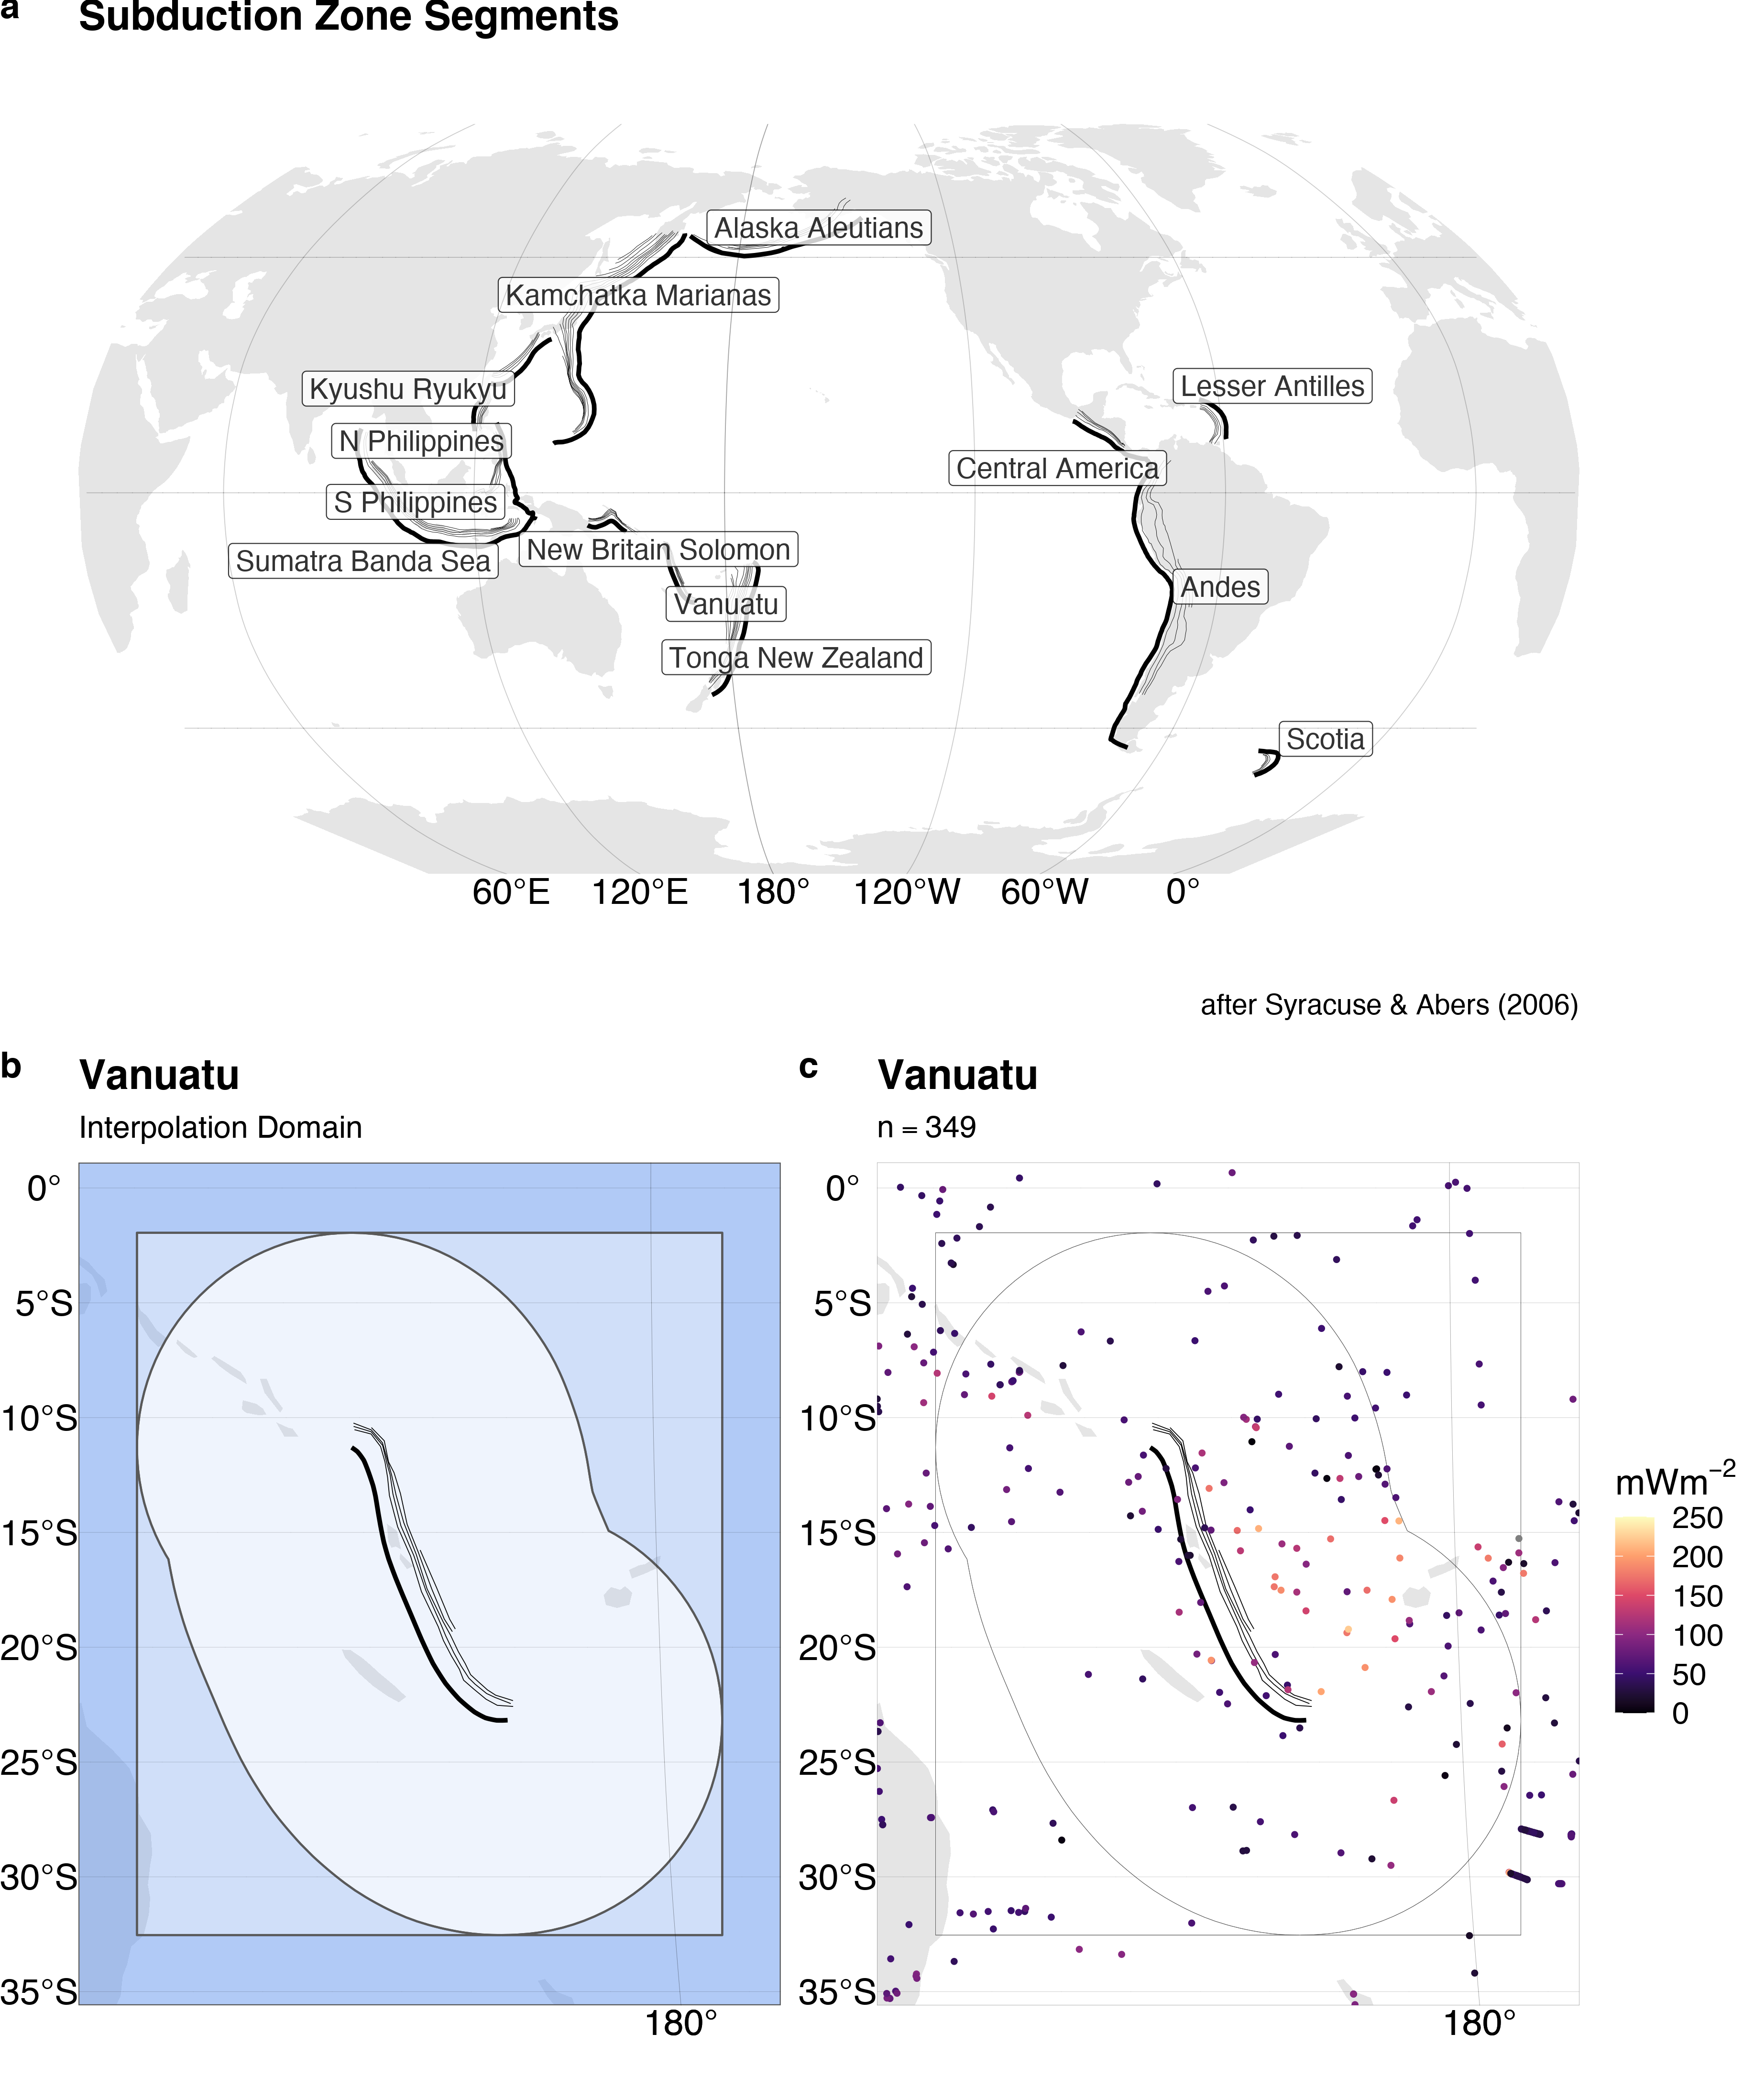
\includegraphics[width=0.95\linewidth,]{../figs/base/segs_comp} 

}

\caption{Subduction zone segments and interpolation domain. (a) Heat flow is interpolated around thirteen subduction zone segments by (b) drawing a 1000km buffer (lightest blue) around each segment and expanding the buffer's bounding box (medium blue) by 10\% on all sides (darkest blue). (c) The NGHF dataset is cropped within the largest rectangle. Data from Syracuse \& Abers (2006) and Lucazeau (2019).}\label{fig:segments}
\end{figure}

\clearpage

\section{Results}

\subsection{Heat Flow Near Subduction Zone Segments}

Summary statistics for surface heat flow observations by subduction zone
segment are given in Table~\ref{tbl:hf.summary.table} and
Figure~\ref{fig:hf.summary.plot}. Surface heat flow is median-centered
around 45-70 \(mWm^{-2}\) and narrowly distributed (excluding outliers)
with inter-quartile ranges (IQR) from 12 to 50 \(mWm^{-2}\) for most
subduction zone segments. Alaska Aleutians is the exception with a
higher median of 184 \(mWm^{-2}\) and broader range (IQR =
\(250~mW^{-2}\)). The whole distributions (including outliers) for all
segments are strongly right-skewed with maximum heat flow values of
several thousand of \(mWm^{-2}\) or more. Heat flow values above 250
\(mWm^{-2}\) are considered geothermal areas by Lucazeau (2019), which
we adopt as a relevant empirical limit for anomalously high heat flow.

\hypertarget{tbl:hf.summary.table}{}
\begin{longtable}[]{@{}lrrrrrrr@{}}
\caption{\label{tbl:hf.summary.table}Heat flow (\(mWm^{-2}\))
observations}\tabularnewline
\toprule
Segment & n & Min & Max & Median & IQR & Mean & Sigma \\
\midrule
\endfirsthead
\toprule
Segment & n & Min & Max & Median & IQR & Mean & Sigma \\
\midrule
\endhead
Alaska Aleutians & 2791 & 4 & 7765 & 184 & 206 & 233 & 345 \\
Andes & 5226 & 7 & 911 & 45 & 50 & 87 & 89 \\
Central America & 5033 & 8 & 911 & 45 & 48 & 88 & 91 \\
Kamchatka Marianas & 3958 & 1 & 25200 & 71 & 48 & 118 & 582 \\
Kyushu Ryukyu & 3247 & 1 & 25200 & 72 & 44 & 126 & 642 \\
Lesser Antilles & 3535 & 13 & 1150 & 41 & 13 & 52 & 50 \\
N. Philippines & 1002 & 3 & 25200 & 72 & 35 & 195 & 1127 \\
New Britain Solomon & 180 & 3 & 174 & 64 & 42 & 69 & 30 \\
S. Philippines & 1444 & 1 & 25200 & 71 & 43 & 158 & 938 \\
Scotia & 72 & 13 & 145 & 76 & 23 & 74 & 28 \\
Sumatra Banda Sea & 3039 & 1 & 1350 & 65 & 47 & 76 & 67 \\
Tonga New Zealand & 507 & 2 & 416 & 54 & 40 & 64 & 45 \\
Vanuatu & 349 & 2 & 283 & 54 & 40 & 64 & 44 \\
\bottomrule
\end{longtable}

\begin{figure}[h]

{\centering 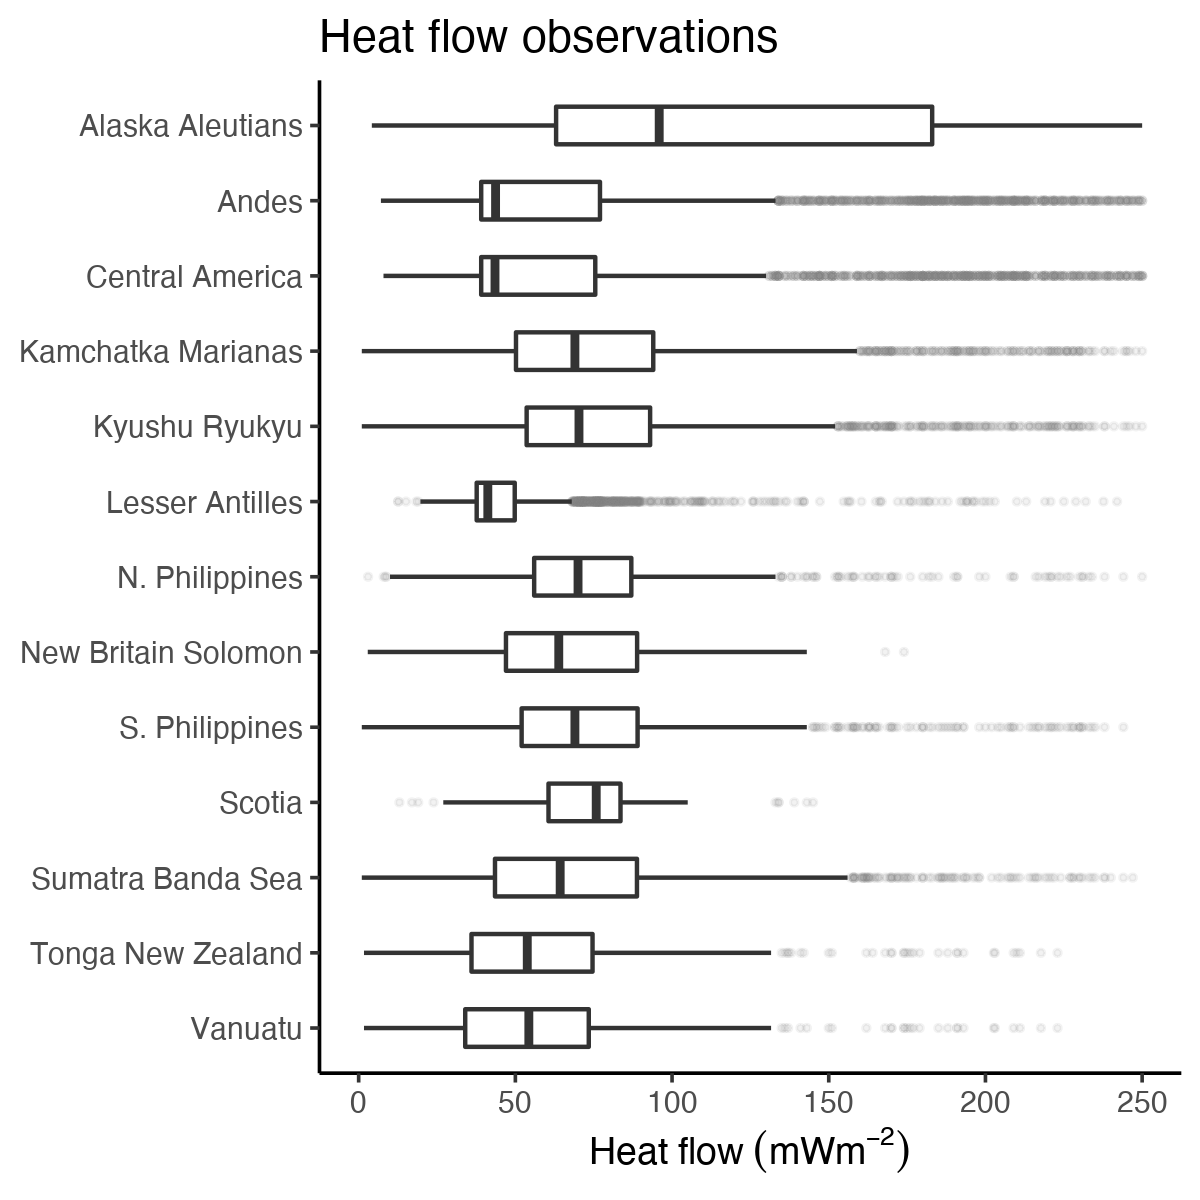
\includegraphics[width=0.6\linewidth,]{../figs/summary/hf_summary} 

}

\caption{Distribution of heat flow observations. Heat flow near most segments is centered around $50~mWm^{-2}$ and highly skewed right (shadowy dot outliers). The skeweness likely represents sampling near geothermal systems, volcanic arcs, or spreading centers. Data from Lucazeau (2019).}\label{fig:hf.summary.plot}
\end{figure}

\subsection{Variogram Models}

The optimal variogram models and associated errors \(C_F(\Theta)\) and
\(C_I(\Theta)\) are given in Table~\ref{tbl:variogram.summary.table}.
Almost twice as many experimental variograms are fit with spherical
models (8) compared to exponential models (5). Variogram model sills
vary substantially among the subduction zone segments between 9 and 1538
\(mWm^{-2}\). Variogram model ranges also vary substantially among
segments from 4 to 1676 \(km\).

No apparent correlation exists between variogram model range and
subduction zone segment length, number of heat flow observations, nor
domain area (Figure~\ref{fig:variogram.summary.plot}). Most subduction
zone segments show spatial dependence of a few hundred kilometers or
less, irrespective of the number of observations or segment size. The
exceptions are Kyushu Ryukyu (range = 1774 \(km\)) and Vanuatu (range =
573 \(km\)), whose model variogram ranges are, perhaps, anomalously
high.

\hypertarget{tbl:variogram.summary.table}{}
\begin{longtable}[]{@{}llrr@{}}
\caption{\label{tbl:variogram.summary.table}Optimal varigram
models}\tabularnewline
\toprule
Segment & Model & Sill \([mWm^{-2}]\) & Range \([km]\) \\
\midrule
\endfirsthead
\toprule
Segment & Model & Sill \([mWm^{-2}]\) & Range \([km]\) \\
\midrule
\endhead
Alaska Aleutians & Sph & 285 & 221 \\
Andes & Sph & 87 & 346 \\
Central America & Sph & 86 & 343 \\
Kamchatka Marianas & Exp & 612 & 271 \\
Kyushu Ryukyu & Sph & 813 & 1774 \\
Lesser Antilles & Exp & 38 & 104 \\
N Philippines & Sph & 1198 & 238 \\
New Britain Solomon & Exp & 29 & 89 \\
S Philippines & Sph & 1026 & 414 \\
Scotia & Exp & 9 & 4 \\
Sumatra Banda Sea & Sph & 67 & 133 \\
Tonga New Zealand & Sph & 47 & 131 \\
Vanuatu & Sph & 48 & 573 \\
\bottomrule
\end{longtable}

\begin{figure}[h]

{\centering 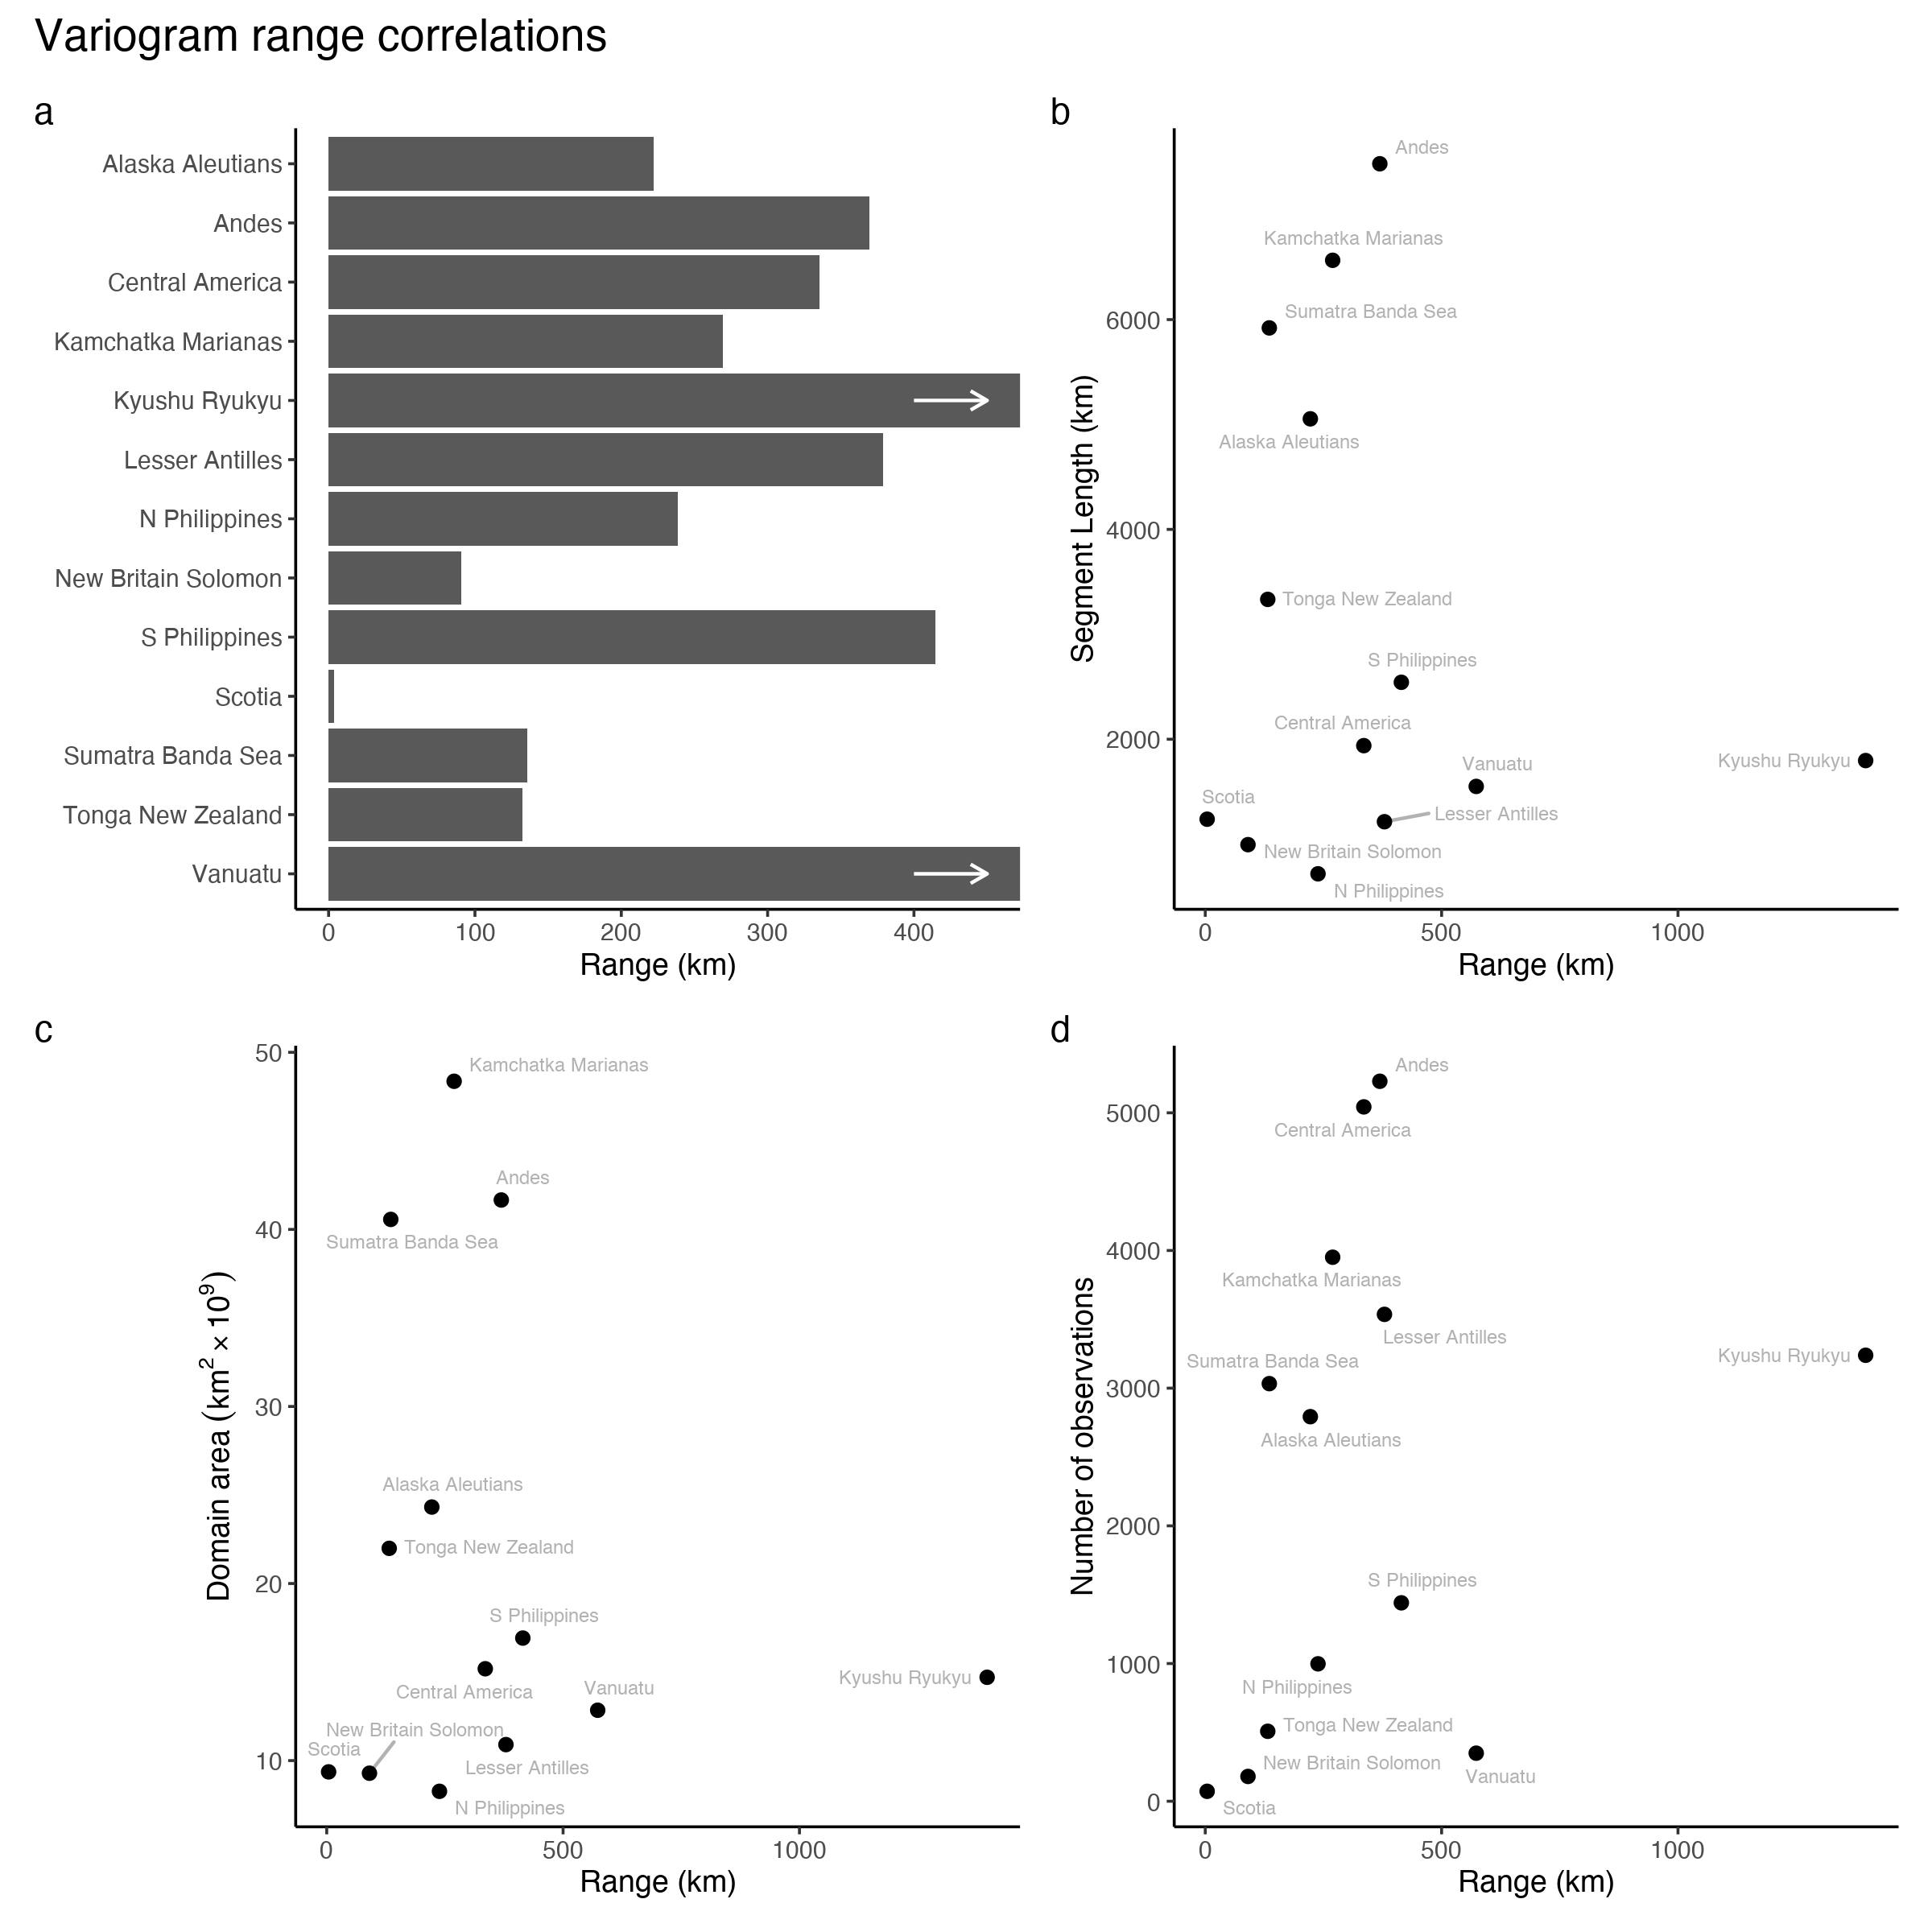
\includegraphics[width=0.95\linewidth,]{../figs/summary/variogram_summary} 

}

\caption{Summary of variogram model ranges and correlations with other features. (a) Variogram model ranges are variable, but generally below 400 km. Variogram model ranges show no correlation with segment length (b), number of heat flow observations (c), nor domain area (d). The spatial dependenc of heat flow is apparently independent of these parameters.}\label{fig:variogram.summary.plot}
\end{figure}

\subsection{Interpolation Comparison}

Summary statistics for the interpolation differences are given in
Table~\ref{tbl:diff.summary.table} and
Figure~\ref{fig:diff.summary.plot}. Note that the difference is taken at
the exact same locations for every prediction. Differences between the
similarity method and Kriging are small for most segments with the
exception of Central America, which shows a broader distribution of
differences than the other segments. The median differences range from
-9 to 7 \(mWm^{-2}\) with inter quartile ranges from 15 to 62
\(mWm^{-2}\). Similar to the distribution of heat flow in these areas,
the minimum and maximum difference in predicted heat flow are extreme
and represent the failure of one method to predict extreme outliers of
the other.

\hypertarget{tbl:diff.summary.table}{}
\begin{longtable}[]{@{}lrrrrrr@{}}
\caption{\label{tbl:diff.summary.table}Predicted heat flow
(\(mWm^{-2}\)) differences}\tabularnewline
\toprule
Segment & Min & Max & Median & IQR & Mean & Sigma \\
\midrule
\endfirsthead
\toprule
Segment & Min & Max & Median & IQR & Mean & Sigma \\
\midrule
\endhead
Alaska Aleutians & -550 & 2659 & -2 & 20 & 3 & 71 \\
Andes & -241 & 2336 & 2 & 35 & 12 & 72 \\
Central America & -242 & 2731 & 8 & 63 & 43 & 147 \\
Kamchatka Marianas & -2434 & 297 & 4 & 15 & 4 & 39 \\
Kyushu Ryukyu & -2435 & 136 & 6 & 24 & 2 & 74 \\
Lesser Antilles & -148 & 566 & 0 & 16 & 5 & 31 \\
N Philippines & -2131 & 283 & 2 & 24 & -1 & 67 \\
New Britain Solomon & -81 & 236 & 2 & 22 & 5 & 20 \\
S Philippines & -273 & 369 & 5 & 26 & 7 & 30 \\
Scotia & -62 & 1001 & -4 & 24 & 5 & 33 \\
Sumatra Banda Sea & -312 & 386 & 0 & 20 & 2 & 20 \\
Tonga New Zealand & -113 & 1695 & -9 & 23 & -2 & 30 \\
Vanuatu & -166 & 1657 & 7 & 27 & 8 & 40 \\
\bottomrule
\end{longtable}

Prediction differences are either approximately normally distributed, or
skewed right. Right skew and a tendency of medians to deviate positively
from zero both reflect a systematic overprediction of heat flow by the
similarity method compared to Kriging
(Figure~\ref{fig:diff.summary.plot}). However, Alaska Aleutians, Scotia,
and Tonga New Zealand have negative median differences. While there is a
tendency for the similarity method to overpredict heat flow compared to
Kriging, it is not true in every case.

\begin{figure}[h]

{\centering 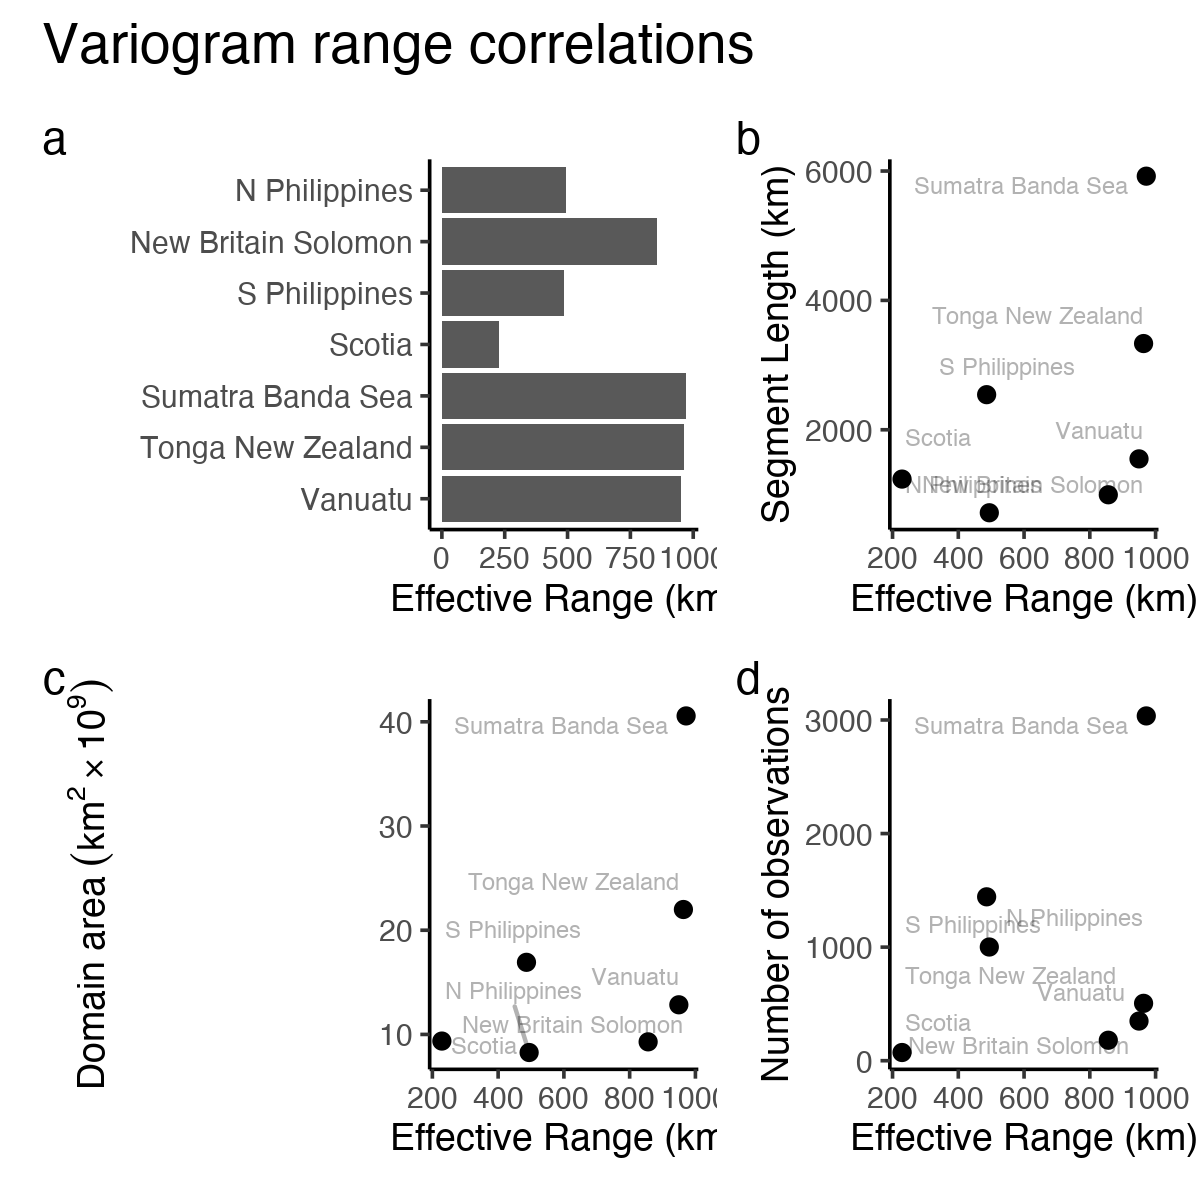
\includegraphics[width=0.6\linewidth,]{../figs/summary/hf_diff_summary} 

}

\caption{Point-by-point differences of predicted heat flow between similarity and Kriging interpolations. The differences for most subduction zone segments are median-centered at or near-zero with IQRs from 16 to 62. Outliers (shadowy dots) extend to extreme positive and negative differences.}\label{fig:diff.summary.plot}
\end{figure}

Notable sources of prediction differences include 1) tectonic features
predicted by similarity that are absent from Kriging or 2) general
discordance between the spatial continuity of heat flow observations and
similarity predictions. For example, high heat flow representing
Galápagos triple junction is predicted by similarity to the SW of the
Central America segment (Figure~\ref{fig:central.america.diff} a).
However, none of the triple junction arms, nor the Galápagos hot spot,
are well defined in the Kriged prediction
(Figure~\ref{fig:central.america.diff} b). The interpolation comparison
for Central America highlights two distinct regions---bright differences
along the arms of the triple junction and muted agreement to the E and
NE of the Cocos Plate (Figure~\ref{fig:central.america.diff} c). Note
the moderate differences within the Cocos Plate in
Figure~\ref{fig:central.america.diff} a where similarity predicts high
heat flow by proximity to the nearby spreading centers, but heat flow in
the region is, in fact, relatively low (compare
Figure~\ref{fig:central.america.diff} a, b, c). Similar discordance
between high similarity predictions and low heat flow observations are
observed in many subduction zone segments, especially near spreading
centers predicted by similarity (e.g. Figure~\ref{fig:andes.comp}; see
sec.~\ref{sec:comps}).

\begin{figure}[h]

{\centering 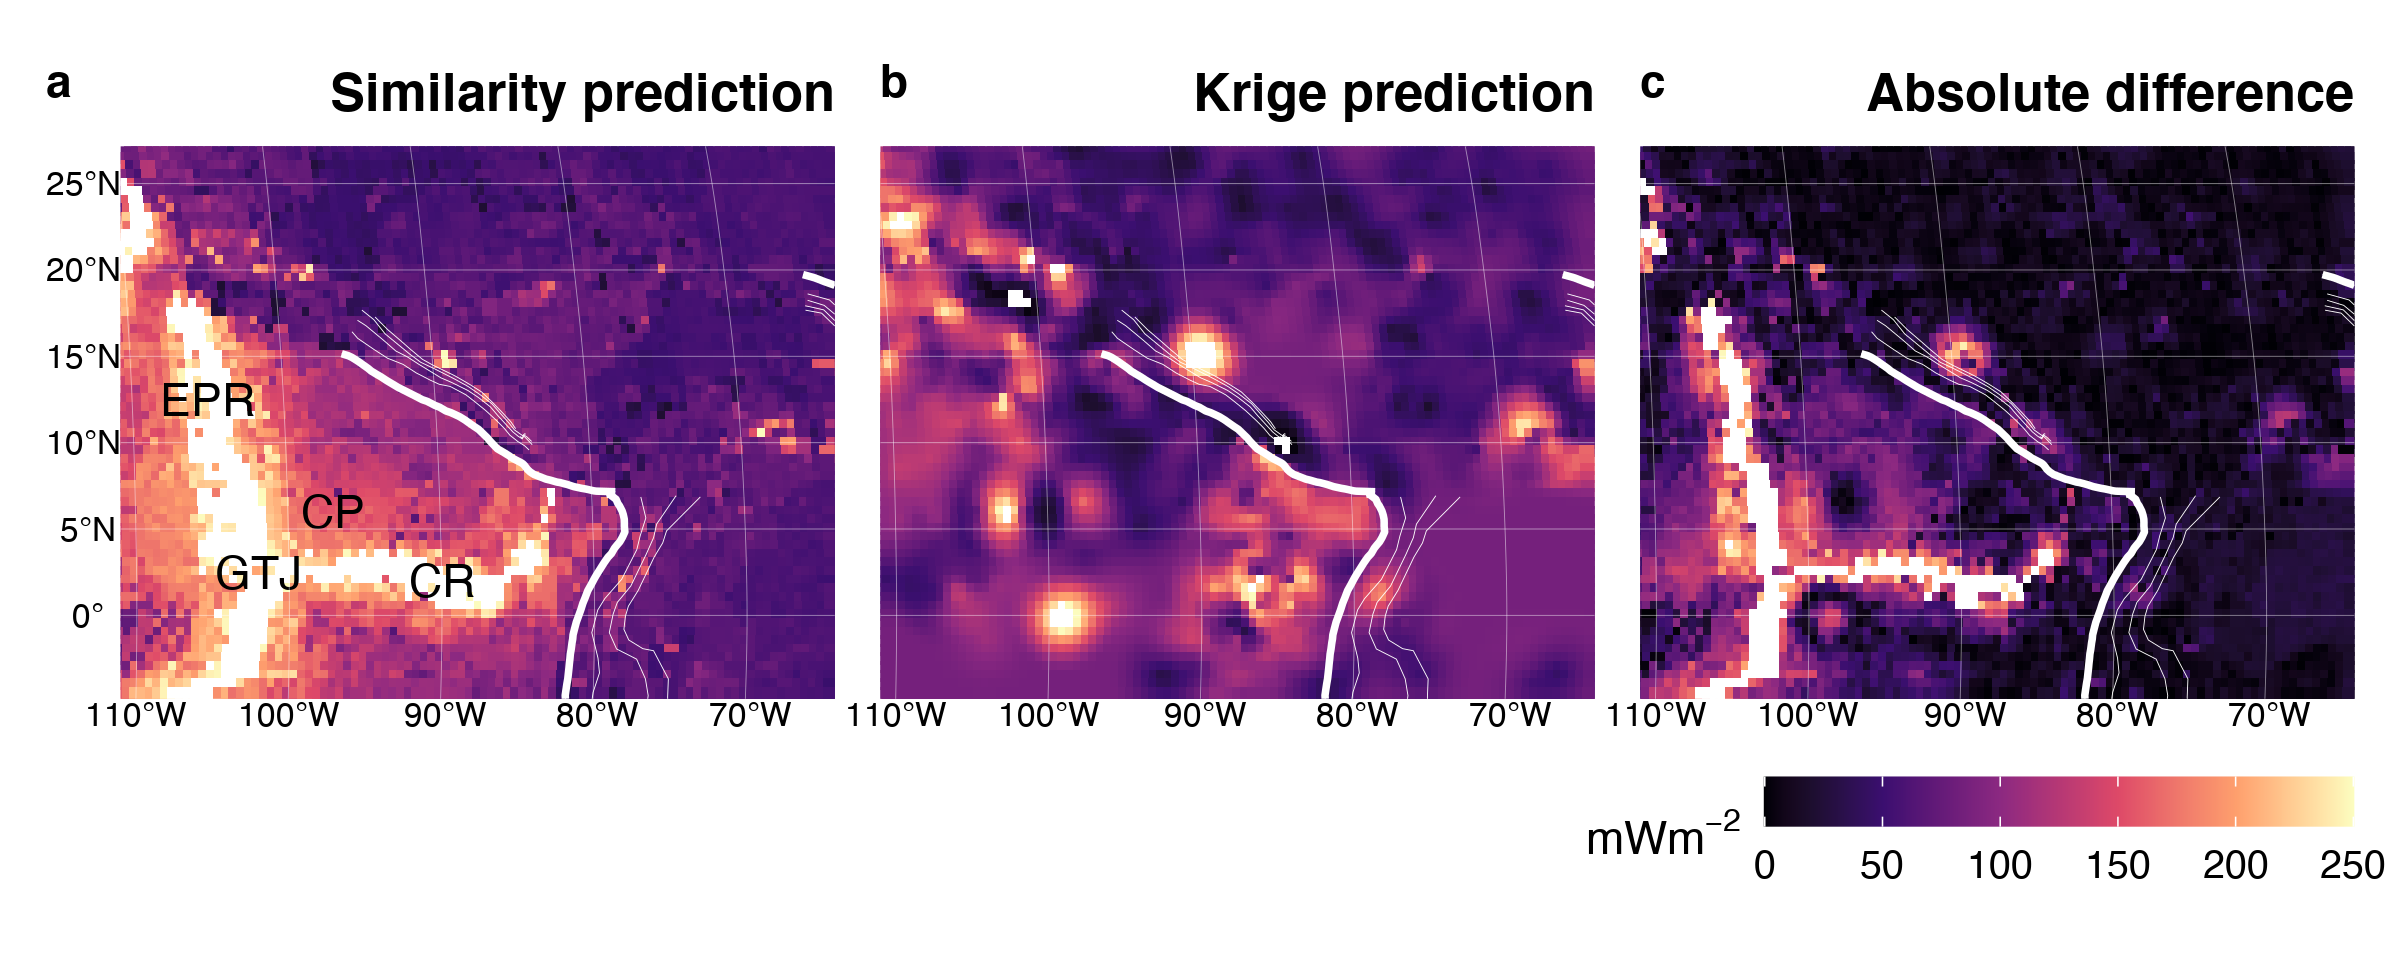
\includegraphics[width=0.95\linewidth,]{../figs/diff/custom/Central_America} 

}

\caption{Similarity vs. Kriging predictions for Central America. The Galápagos triple junction (GTJ), East Pacific Rise (EPR), and Cocos Ridge (CR) are predicted by similarity (a), but not by Kriging (b). Note the moderate difference between predictions within the Cocos Plate (CP) where similarity predicts high heat flow but observations are low (c). Bold and thin white lines represent the subduction zone segment boundary and plate depth, respectively, as defined by Syracuse \& Abers (2006). Heat flow data and similarity prediction from Lucazeau (2019).}\label{fig:central.america.diff}
\end{figure}

On the other side of the Caribbean Plate, near the Lesser Antilles
segment, similarity and Kriging predictions show good agreement. The
Mid-Atlantic Ridge to the E appears in both predictions
(Figure~\ref{fig:lesser.antilles.diff} a, b). The spreading center is
better defined with Kriging in this case, as compared to the Galápagos
triple junction, because the observational density and spatial coverage
near the Lesser Antilles segment are sufficiently high and continuous
near the Mid-Atlantic Ridge (see sec.~\ref{sec:comps}). However, the
comparison still highlight spreading centers as similarity tends to
predict higher heat flow than observations.

\begin{figure}[h]

{\centering 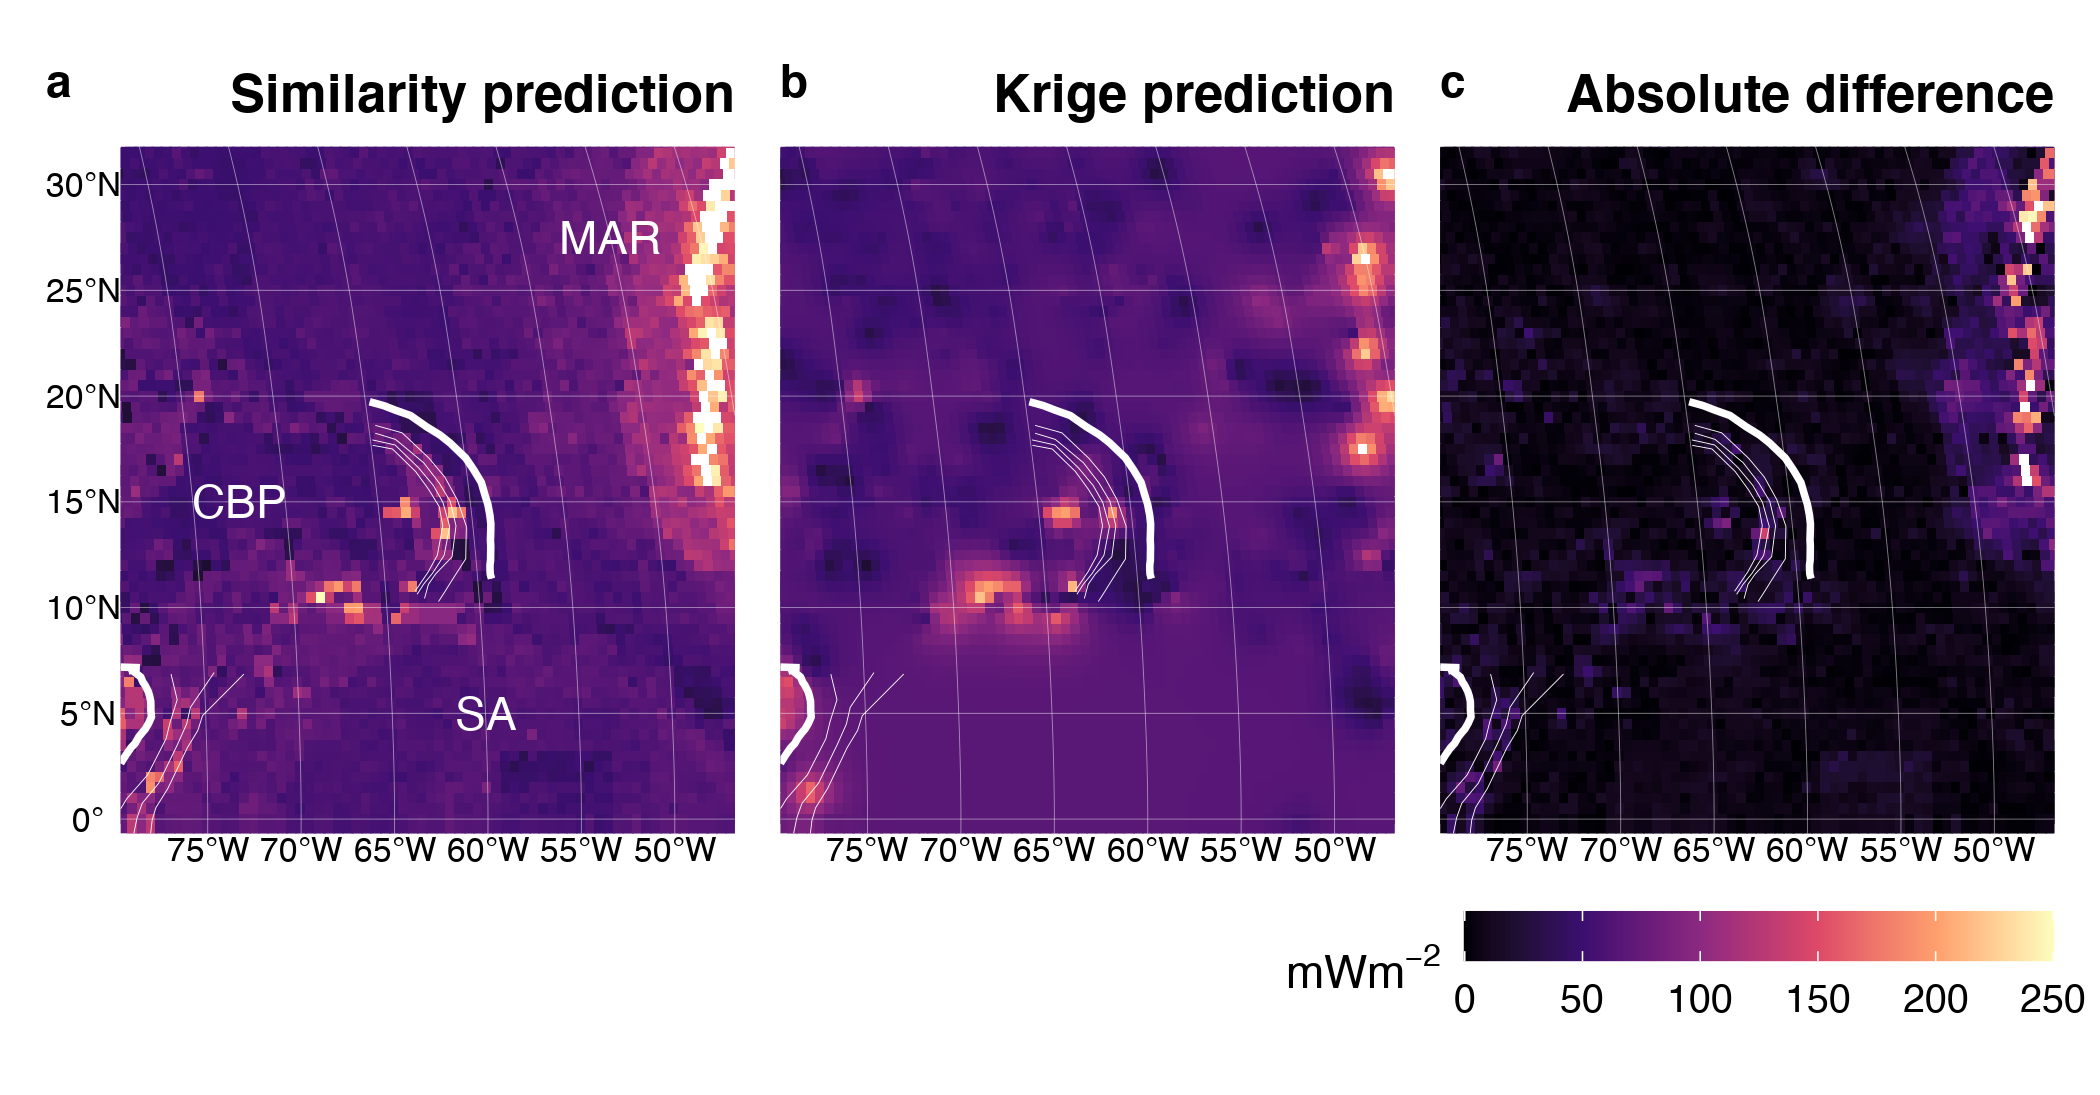
\includegraphics[width=0.95\linewidth,]{../figs/diff/custom/Lesser_Antilles} 

}

\caption{Similarity vs. Kriging predictions for the Lesser Antilles. The Mid-Atlantic Ridge (MAR) predicted by similarity (a) is also defined by Kriging (b) because of adequate observational density and spatial coverage near the spreading center. Good agreement between similarity and Kriging exist for the entire domain (c). CBP = Caribbean Plate, SA = South America. Bold and thin white lines represent the subduction zone segment boundary and plate depth, respectively, as defined by Syracuse \& Abers (2006). Heat flow data and similarity prediction from Lucazeau (2019).}\label{fig:lesser.antilles.diff}
\end{figure}

Another example of good agreement between similarity and Kriging are
interpolations near the Sumatra Banda Sea segment
(Figure~\ref{fig:sumatra.banda.sea.diff};
Figure~\ref{fig:sumatra.banda.sea.comp}). Note the textural and
structural complexity predicted by similarity
(Figure~\ref{fig:sumatra.banda.sea.diff} a) compared to the smooth
featureless Kriging predictions (Figure~\ref{fig:sumatra.banda.sea.diff}
b). Despite the textural and structural differences, the difference
between similarity and Kriging within the Sunda Plate, Australian Plate,
and W Philippine Sea Plate is small
(Figure~\ref{fig:sumatra.banda.sea.diff} c).

\begin{figure}[h]

{\centering 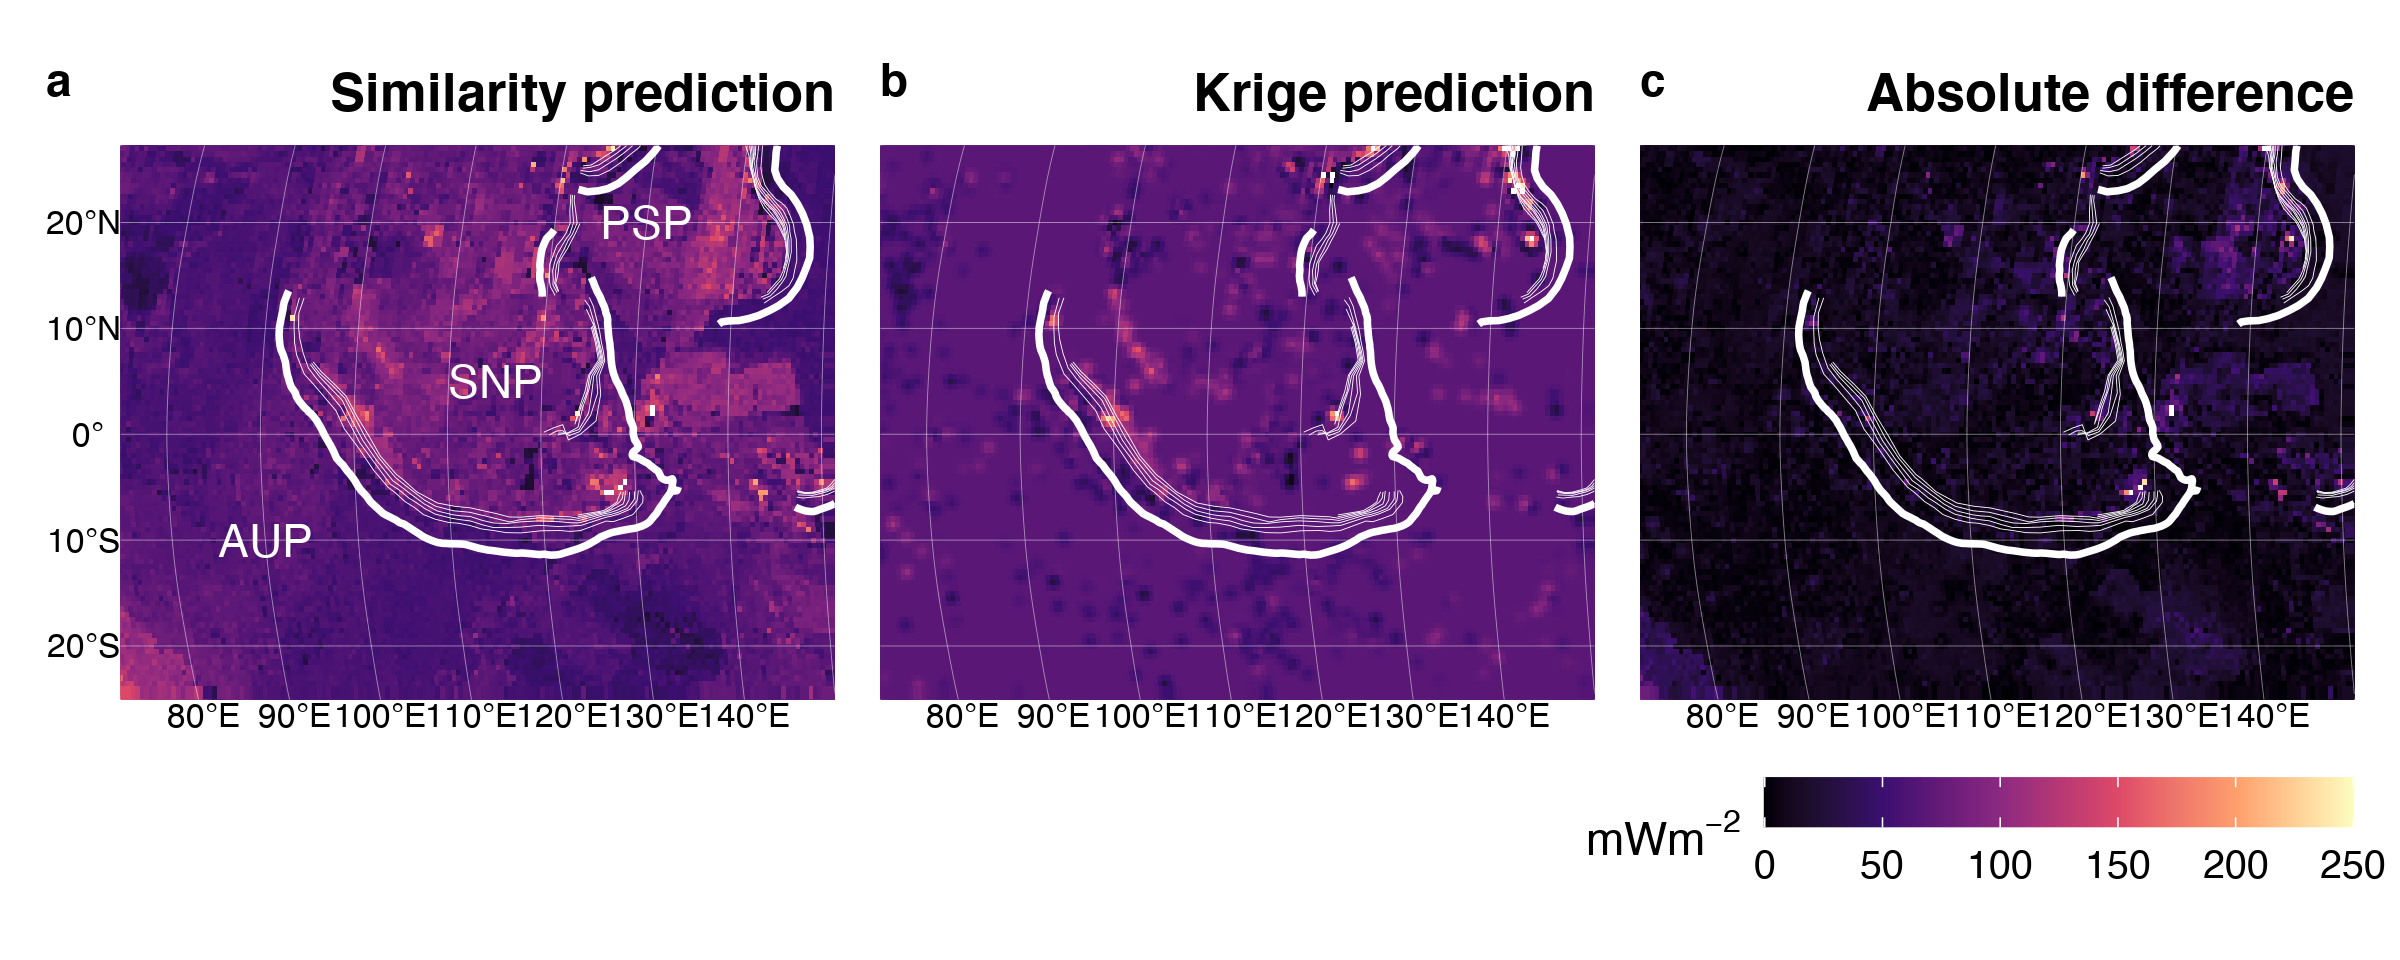
\includegraphics[width=0.95\linewidth,]{../figs/diff/custom/Sumatra_Banda_Sea} 

}

\caption{Similarity vs. Kriging predictions for Sumatra Banda Sea. Similarity predictions are texutrally and structurally complex (a), while Kriging is smooth and featureless (b). Despite the textural and structural difference, the interpolations are similar, especially within the Sunda Plate (SNP), Australian Plate (AUP) and W Philippine Sea Plate (PSP). Bold and thin white lines represent the subduction zone segment boundary and plate depth, respectively, as defined by Syracuse \& Abers (2006). Heat flow data and similarity prediction from Lucazeau (2019).}\label{fig:sumatra.banda.sea.diff}
\end{figure}

Heat flow predictions near the Scotia segment illustrate a case where
heat flow observations are incredibly sparse. Similarity predicts high
heat flow from the East Scotia Ridge (ESR) and the WSW-ENE trending
transform boundary separating the Scotia and Sandwich Plates from the
Antartic Plate (Figure~\ref{fig:scotia.diff} a).
Figure~\ref{fig:scotia.diff} b appears featureless because very few heat
flow observations (n = 72) define a flat experimental variogram for all
lag distances greater than four kilometers (no spatial dependence beyond
4 km, Table~\ref{tbl:variogram.summary.table};
Figure~\ref{fig:scotia.comp}). Kriging predicts the expected (mean) heat
flow value for the entire domain (Figure~\ref{fig:scotia.diff} b), in
this case, according to Equation~\ref{eq:linestimate}. Interestingly,
the expected heat flow is a fine predictor for most of the ocean basin,
except near the spreading center and transform fault
(Figure~\ref{fig:scotia.diff} c). The New Britain Solomon segment shows
a similar comparison (Figure~\ref{fig:new.britain.solomon.comp}) with
good agreement between similarity and Kriging despite very few heat flow
observations, little spatial dependence (small variogram range), and a
featureless Kriged interpolation.

\begin{figure}[h]

{\centering 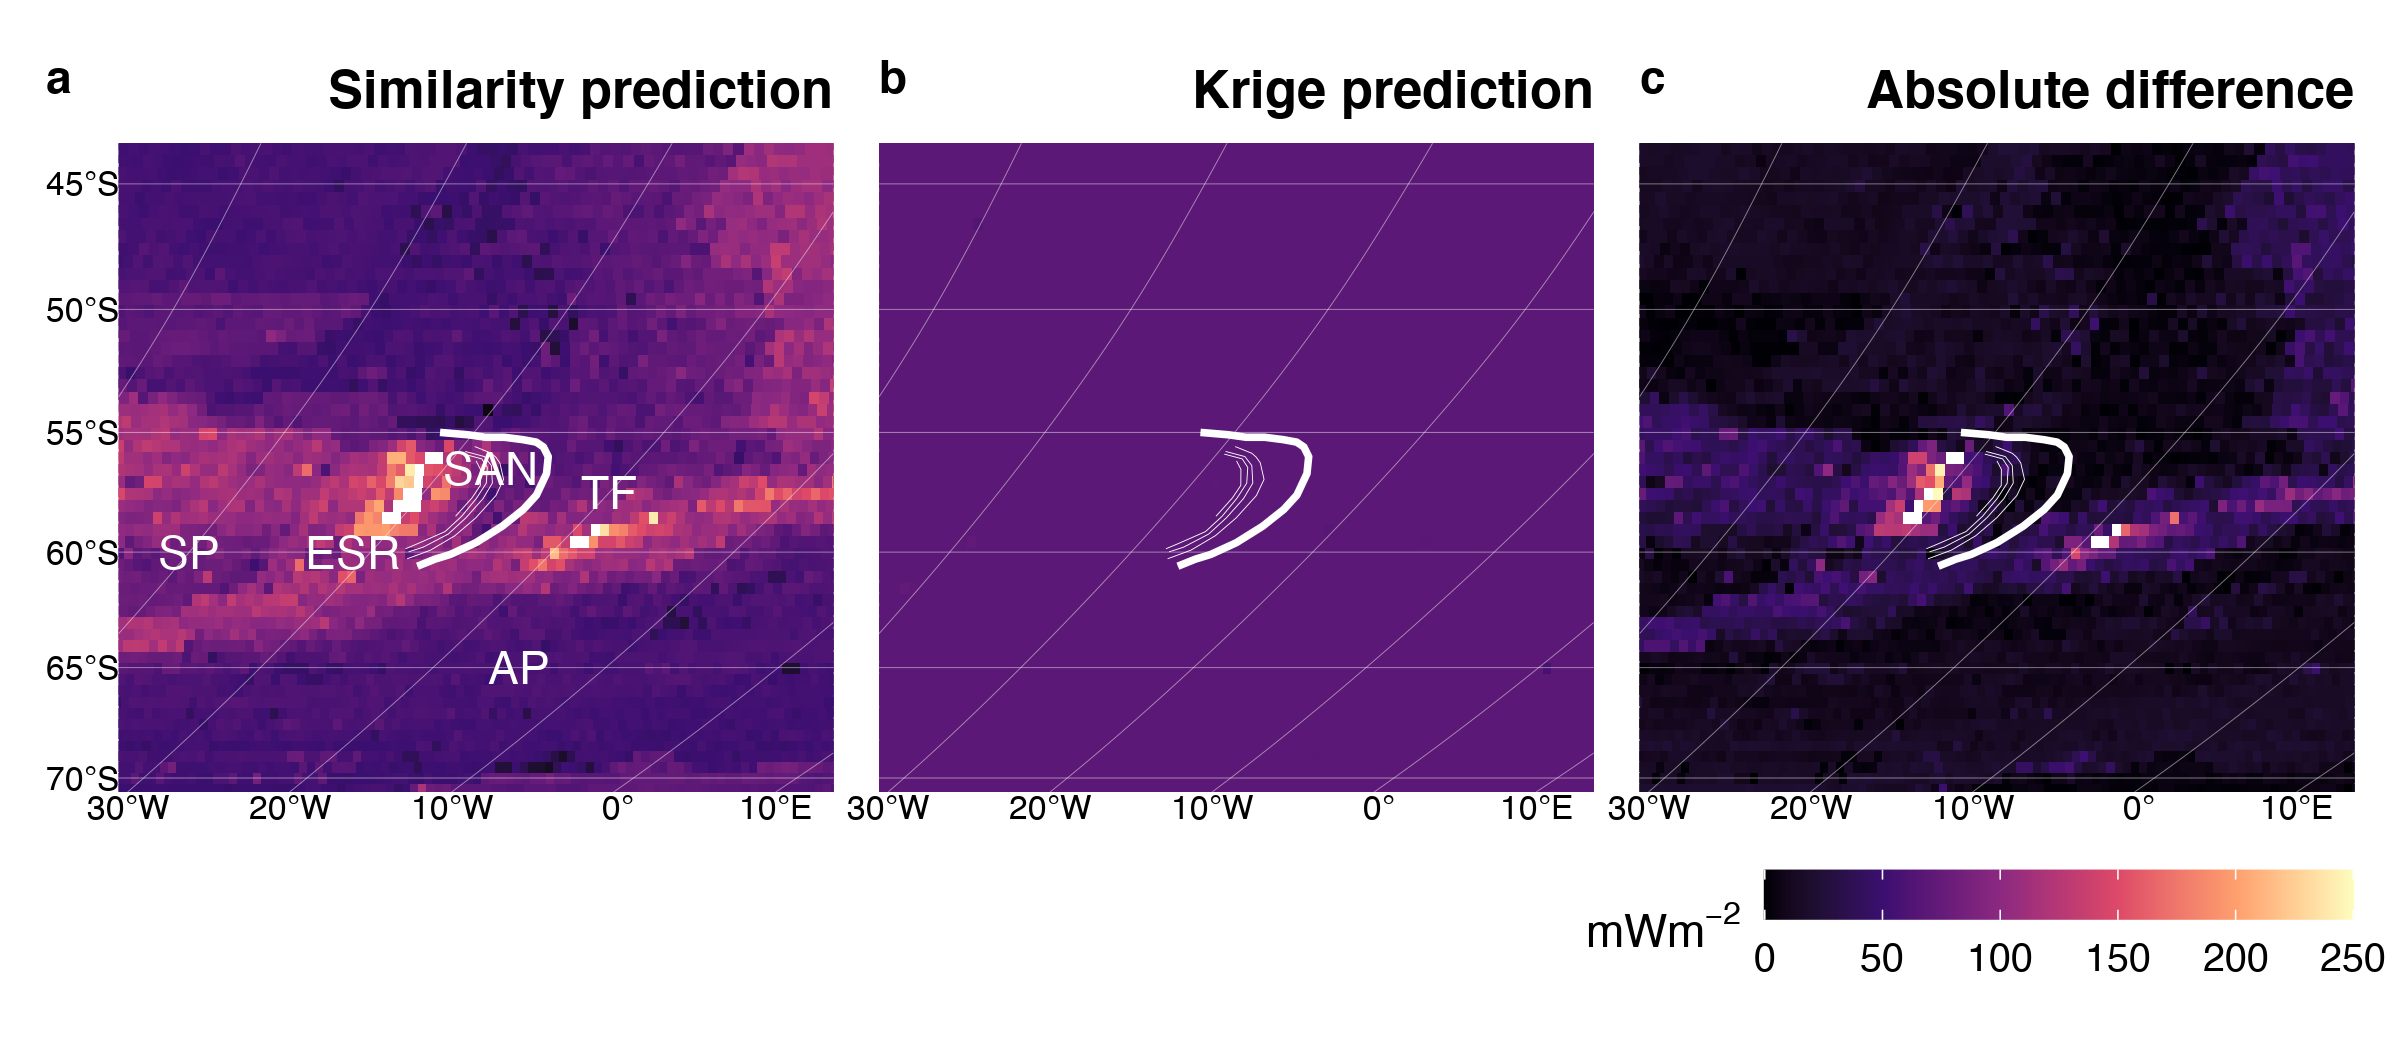
\includegraphics[width=0.95\linewidth,]{../figs/diff/custom/Scotia} 

}

\caption{Similarity vs. Kriging predictions for Scotia. (a) Similarity predicts high heat flow for two tectonic features, the East Scotia Ridge (ESR) and a transform fault (TF) separating the Scotia and Sandwich Plates (SP, SAN) from the Antartic Plate (AP). Kriging (b) is featureless because of incredibly sparse data. Despite few heat flow observations. Kriging predictions are only significantly different than similarity predictions near the ESR and transform fault (c). Bold and thin white lines represent the subduction zone segment boundary and plate depth, respectively, as defined by Syracuse \& Abers (2006). Heat flow data and similarity prediction from Lucazeau (2019).}\label{fig:scotia.diff}
\end{figure}

While similarity tends to define tectonic features and Kriging tends to
smooth out tectonic features, we find the opposite pattern within the
tectonically-complex region near Vanuatu. Similarity predicts the N-S
trending spreading center separating the New Hebrides plate from the
Balmoral Reef and Conway Reef microplates (Figure~\ref{fig:vanuatu.diff}
a). However, heat flow observations are sufficiently dense and
continuous to partially resolve the short ridge segments and transform
faults outlining the microplates between Vanuatu and the Tonga New
Zealand segments by Kriging (Figure~\ref{fig:vanuatu.diff} b). The
differences (Figure~\ref{fig:vanuatu.diff} c) are difficult to interpret
because of the somewhat random discordance between interpolation
methods.

\begin{figure}[h]

{\centering 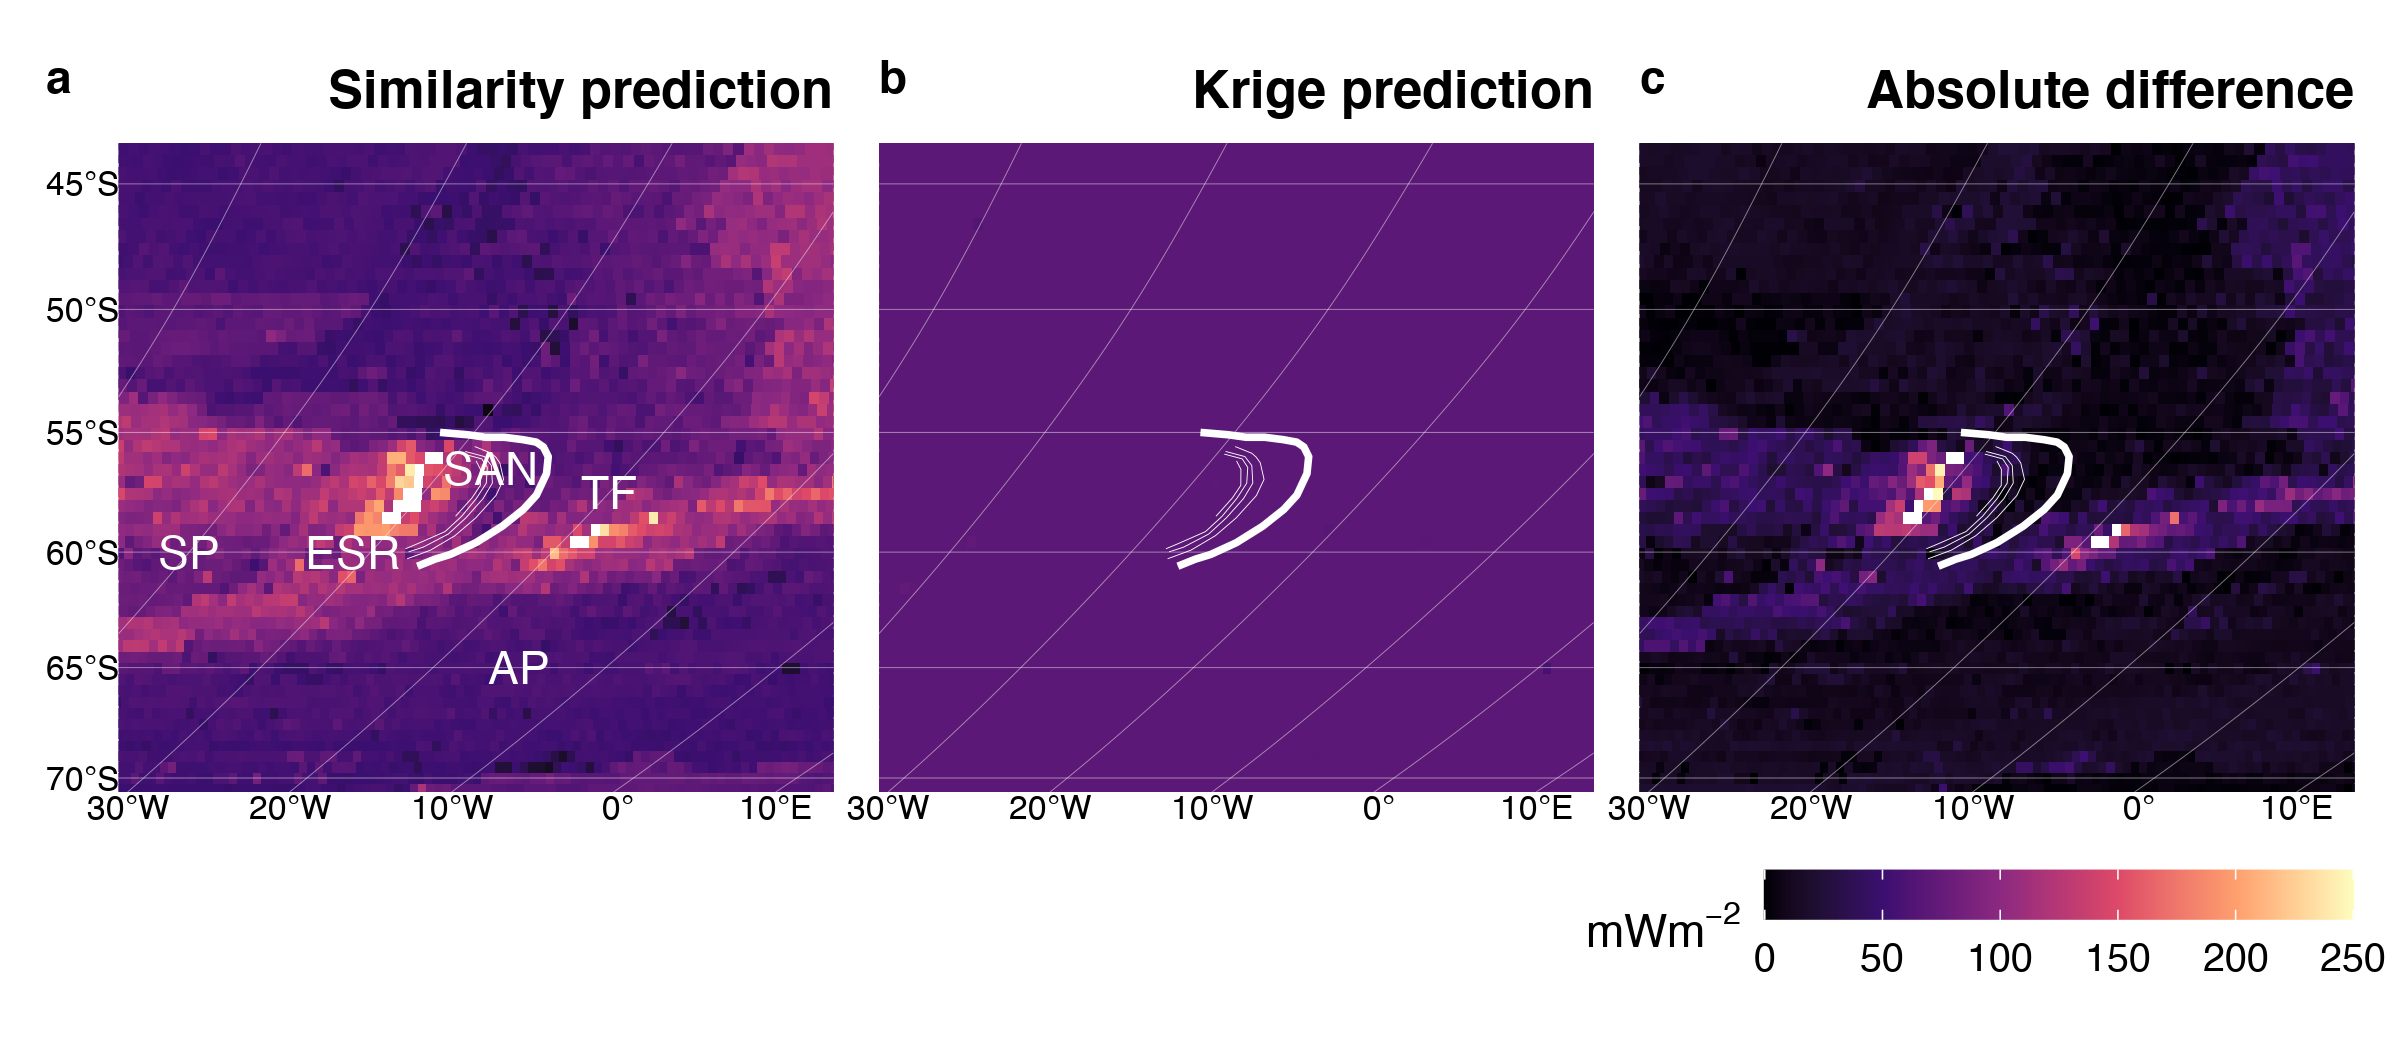
\includegraphics[width=0.95\linewidth,]{../figs/diff/custom/Scotia} 

}

\caption{Similarity vs. Kriging predictions for Vanuatu. (a) Similarity resolved the spreading center separating the New Hebrides Plate (NHP) from the Balmoral Reef (BR) and Conway Reef (CR) microplates. Sufficient heat flow observations allow Kriging to resolve additional ridge segments and transform faults outlining BR and CR (b). The difference between similarity and Kriging (c) is discordant and difficult to interpret. Bold and thin white lines represent the subduction zone segment boundary and plate depth, respectively, as defined by Syracuse \& Abers (2006). Heat flow data and similarity prediction from Lucazeau (2019).}\label{fig:vanuatu.diff}
\end{figure}

\clearpage

\section{Discussion}

\subsection{Kriging Optimization}

Variogram model ranges characterize the maximum separation distance at
which pairs of points are spatially dependent (Matheron, 1963).
Therefore, the range is the most important parameter to evaluate when
considering spatial continuity of heat flow.

\subsection{The First and Third Laws of Geography}

The Third Law of Geography states that \emph{two points with similar
geographic configurations should have similar values}. In the context of
heat flow near subduction systems and associated spreading centers, the
Third Law produces interpolations that highlight discrete tectonic
features (spreading centers and large fault systems) with complex
regional texture. At first glance the textural complexity may be
misconstrued as realistic interpolations, but is merely an artifact of
the similarity method. The texture predicted by similarity is artificial
insofar as it does not represent spatial changes in surface heat flow.
Rather each prediction location represents an independent assignment of
heat flow by association to all other locations with similar geographic
configurations (Goutorbe et al., 2011; Lucazeau, 2019; Zhu et al.,
2018). The extent to which similarity predictions represent real changes
of heat flow in space is entirely dependent on the reliability of the
Third Law, the quality of the physical proxies, and the selected
combination of proxies used for interpolation.

We note a few inconsistencies with Lucazeau (2019)'s similarity
predictions in the domains considered in this study. First, Lucazeau
(2019)'s predictions systematically overpredict heat flow near spreading
centers, justifying an adjustment to their algorithm. Second, known
tectonic features within the tectonically-complex region near Vanuatu
may be better resolved by Kriging than Lucazeau (2019)'s predictions. It
is important to note, however, that Vanuatu is the only case where
Kriging resolves tectonic features that similarity does not; the trend
is otherwise opposite. Moreover, the inconsistencies near Vanuatu do not
imply algorithmic issues and can likely be resolved by similarity using
a finer-scale grid.

The more important inconsistencies are general discordance between
similarity predictions and observations. Disagreements with observations
imply failures of the Third Law, which are not easily correctable
algorithmically. Cross-validation statistics given by Lucazeau (2019)
demonstrate good agreement with observations in general. The
cross-validation error may be sufficiently small for calculating global
heat flux and probing other relevant questions on the global scale.
However, testing hypotheses which require sampling heat flow on the
subduction zone segment scale should carefully consider where
predictions and observations differ, regardless of the interpolation
method (discussed further below).

Unlike the Third Law, the First Law of Geography by definition does not
allow discordance between predictions and observations. This fact can be
colloquially stated as \emph{everything is related, but nearer things
are more related (and points at the exact same location are perfectly
related)}. More formally, the covariance of two points at the same
location must be zero. Comparing the First and Third Laws reveals
further asymmetry in the sources of errors. Sources of interpolation
error include: 1) quality of heat flow observations (First \& Third
Law), 2) variance of predictions at unknown locations (First \& Third
Law), 3) residuals of predictions at known locations (Third Law), 4)
Kriging weights (variogram model; First Law), 5) variances of physical
proxies (Third Law), 6) combinations of physical proxies (Third Law), 7)
similarity weights (similarity model; Third Law). Interpolation
uncertainty is easier to conceptualize and quantify for First Law
interpolations than Third Law interpolations.

Arguments in favor of First or Third Law interpolations, however, are
not easily generalized. Third Law interpolations are justified in cases
with inadequate heat flow observations (e.g.~Scotia and New Britain
Solomon). First Law interpolations are arguably more favorable in all
cases with adequate heat flow observations because 1) enough
observations will resolve important features, 2) spatial dependency is
respected, and 3) there are fewer sources of uncertainty. However, it is
difficult to know what ``adequate'' observational density and spatial
coverage are \emph{a priori}. In any case, it may not be feasible to
achieve adequate observational density and spatial coverage due to time
and budget constraints. Therefore, hypotheses and sampling strategies
should be constructed with careful consideration of whether First or
Third Law interpolations are more appropriate on a case-by-case basis.

\subsection{Heat Flow Sampling and Hypothesis Testing}

Testing hypotheses relating to subduction dynamics require sampling of
heat flow in order to apply statistical models. Sampling in previous
work commonly uses a three-part strategy: 1) draw a cross-section line
perpendicular to the trench, 2) draw a rectangle with arbitrary width
bisected by the section line, 3) gather all heat flow observations
within the rectangle and project them onto the section line (e.g.,
Currie et al., 2004; Currie \& Hyndman, 2006; Hyndman et al., 2005; Wada
\& Wang, 2009). This sampling strategy is simple and most effective if
measurements along section lines are equally spaced with high spatial
density. Observations along straight transects perpendicular to
trenches, however, are rare in the NGHF except for a few studies
e.g.~near the Lesser Antilles and Sumatra Banda Sea segments,
\ref{fig:NGHF}, (Lucazeau, 2019). There are additional limitations to
this method, including: 1) the method increasingly violates the First
Law as the size of the sampling rectangle increases---projecting more
disparate points onto the section line---and 2) sampling must be
repeated many times along strike to fully characterize the spatial
distribution of heat flow near subduction zone segments. Despite these
limitations, previous work use single transects to characterize whole
subduction zones, which are then compared to make broad claims about
global subduction dynamics (e.g., Currie et al., 2004; Currie \&
Hyndman, 2006; Hyndman et al., 2005; Kerswell et al., 2020; Wada \&
Wang, 2009).

Hypotheses such as common depths of slab-mantle mechanical coupling and
commonly thin backarc lithospheres (Currie et al., 2004; Currie \&
Hyndman, 2006; Furukawa, 1993; Kerswell et al., 2020; Wada \& Wang,
2009) cannot be adequately tested using the single-transect method
described above. First and Third Law interpolations show that spatial
variance in heat flow near subduction zone segments is simply too high
to support any claim that subduction dynamics are operating on vastly
similar spatiotemporal scales either within or among subduction zone
segments. For example, sampling along section lines offset at 50 \(km\)
from previously published section lines (Currie et al., 2004; Currie \&
Hyndman, 2006; Furukawa, 1993; Wada \& Wang, 2009) is unlikely to
reproduce results. Insofar as heat flow can reliably answer questions
about subduction zone dynamics in space and time, hypothesis must be
qualified with sampling techniques that consider the appropriate number
of dimensions for the question being asked. Sampling and projection onto
a one-dimensional section line is insufficient for testing hypotheses
about the two-dimensional distribution of dynamic processes.

In simple terms, heat flow interpolations near subduction zones imply
either 1) disorganized subsurface structure and spatially heterogeneous
dynamics, or 2) broad obfuscation of subsurface structure and dynamics
by near-surface processes. Therefore we encourage a more
antireductionist view of subduction zone dynamics. We point out that
while testing of many important subduction-related questions may not be
feasible with the current global dataset, the idea of broad dynamic
commonality among subduction systems does not hold up to scrutiny from
the heat flow interpolations presented here.

Important question arise from the present interpolations:

\begin{enumerate}
\def\labelenumi{\arabic{enumi}.}
\item
  Is collecting more heat flow data beneficial for future subduction
  zone research?
\item
  Where should data collection efforts be focused?
\item
  Should First or Third Law methods be favored when prioritizing data
  collection targets?
\end{enumerate}

\section{Conclusions}

\acknowledgments

\section*{Appendix}
\addcontentsline{toc}{section}{Appendix}

\hypertarget{sec:comps}{%
\subsection*{Heat flow observations and predictions}\label{sec:comps}}
\addcontentsline{toc}{subsection}{Heat flow observations and
predictions}

\begin{figure}[h]

{\centering 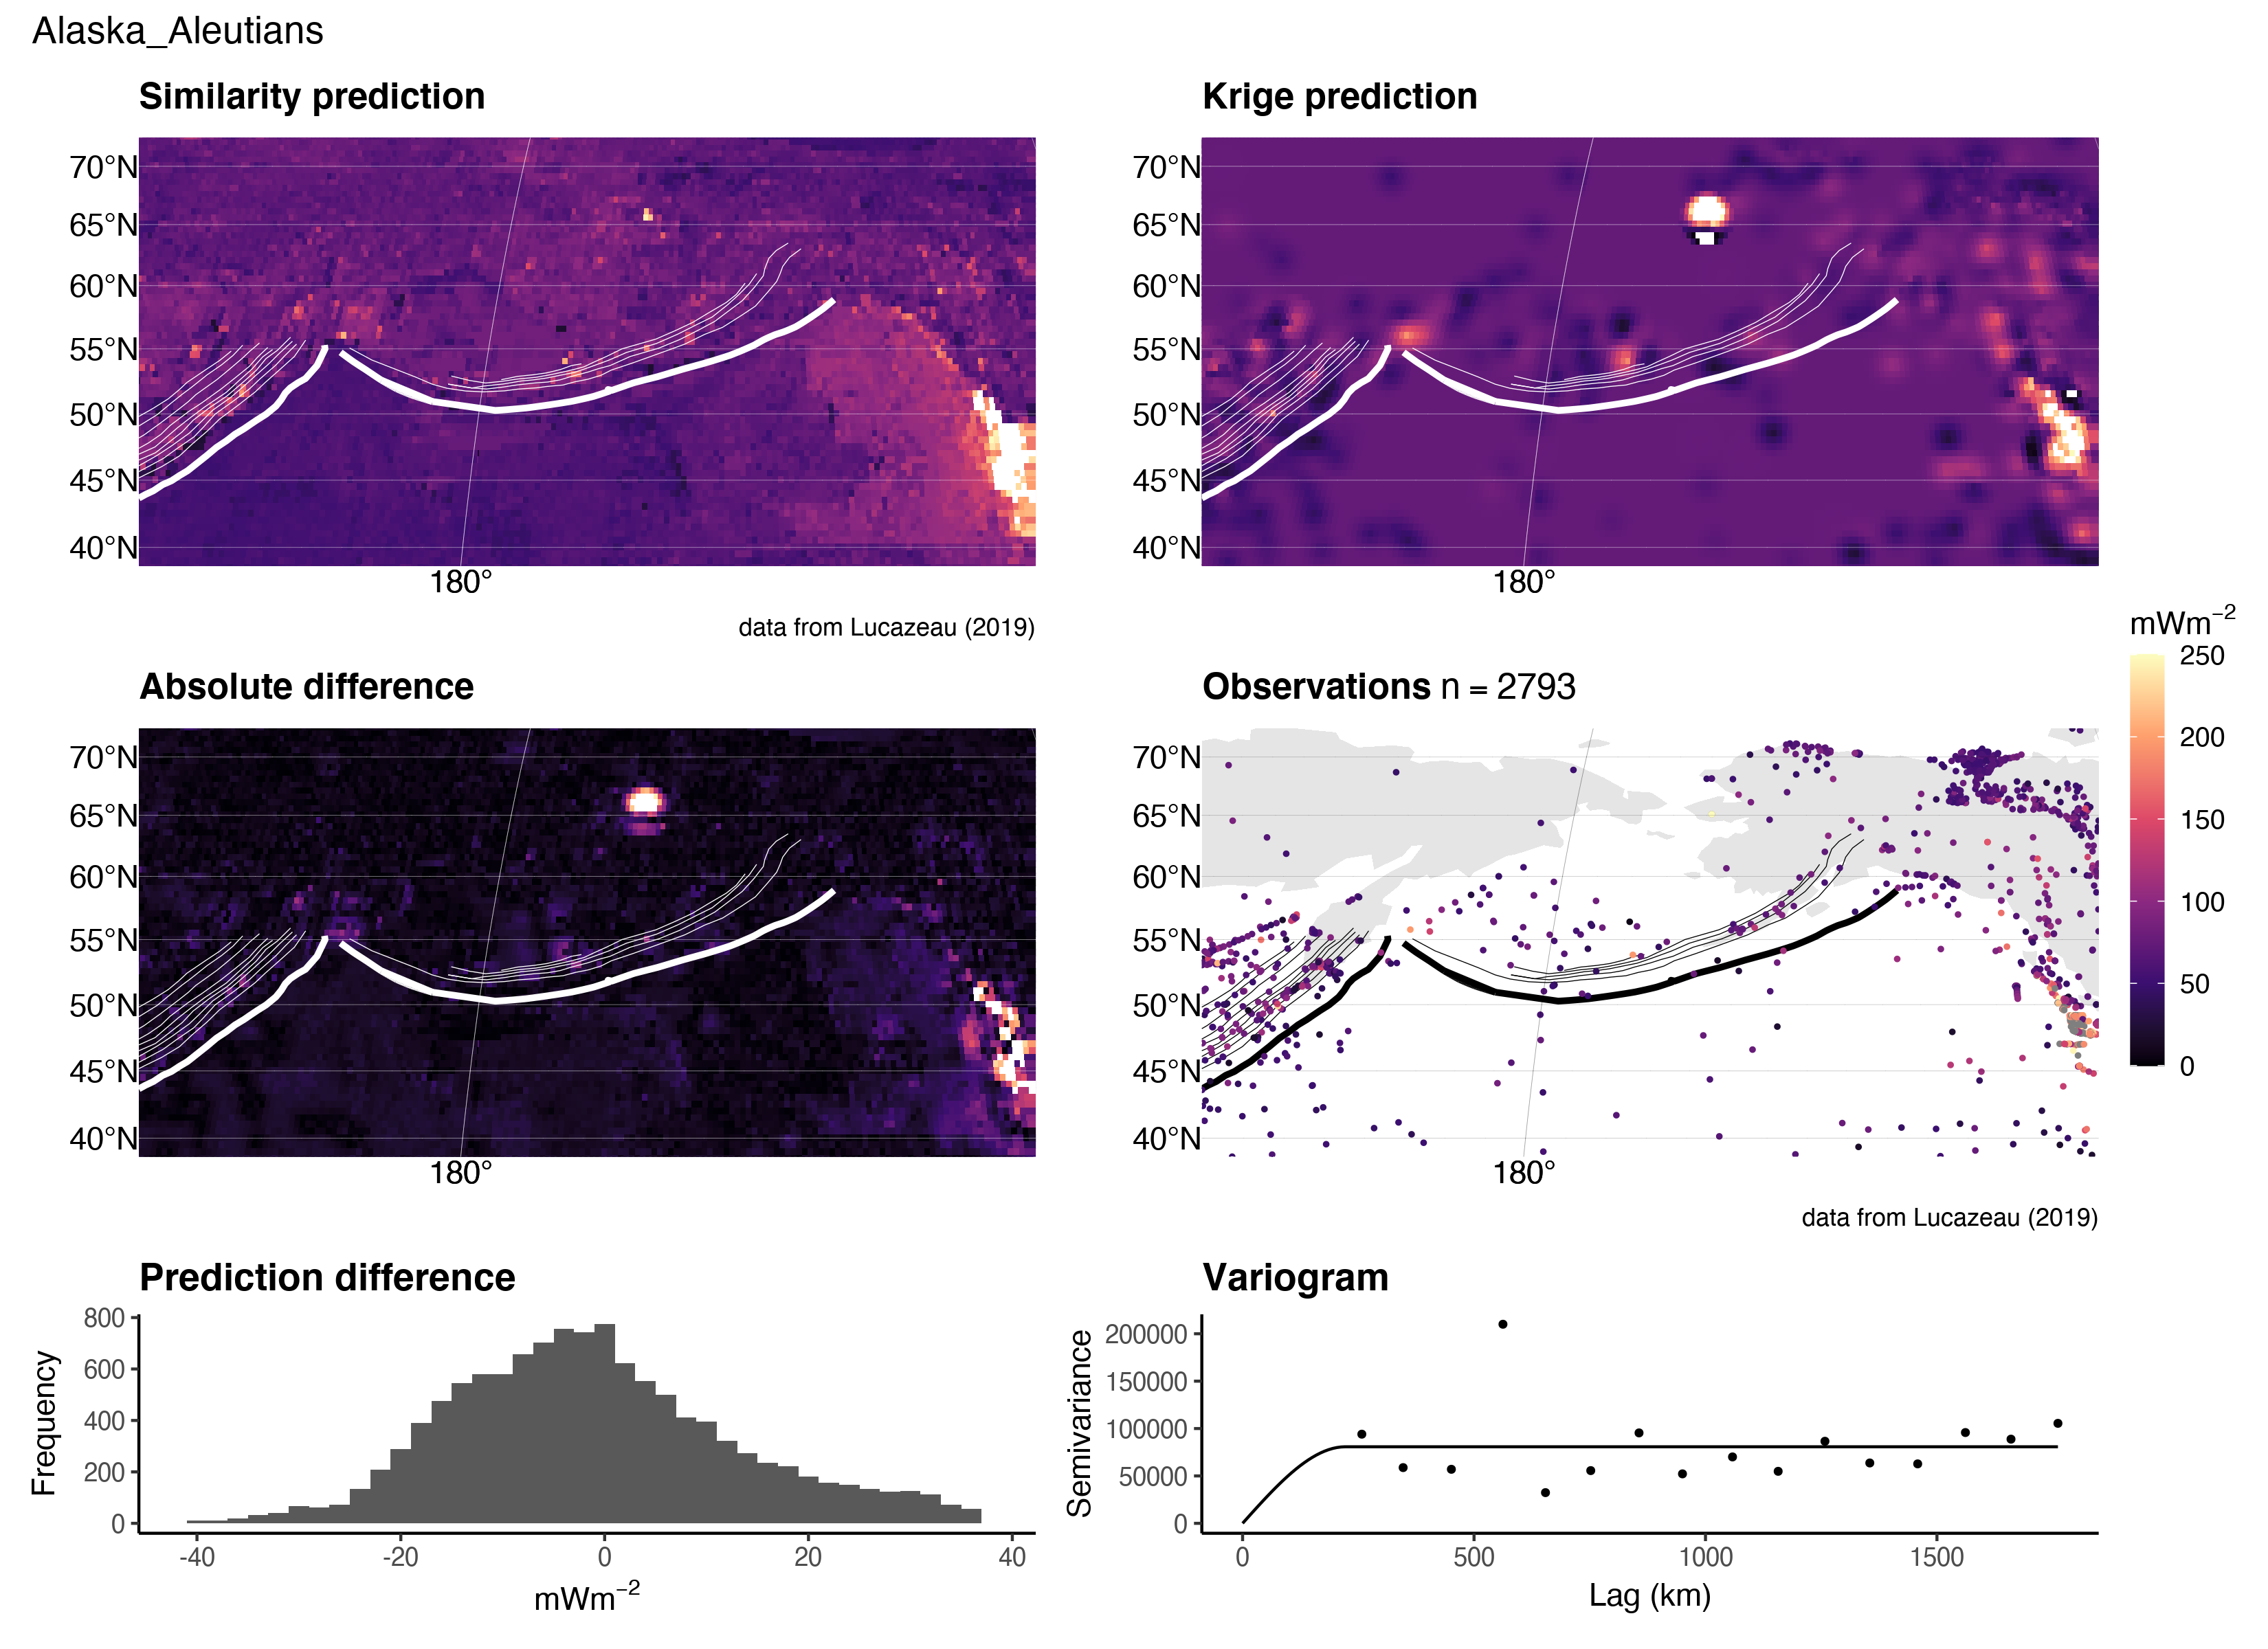
\includegraphics[width=0.95\linewidth,]{../figs/diff/comp/Alaska_Aleutians} 

}

\caption{Similarity vs. Kriging predictions for Alaska Aleutians.}\label{fig:alaska.comp}
\end{figure}

\begin{figure}[h]

{\centering 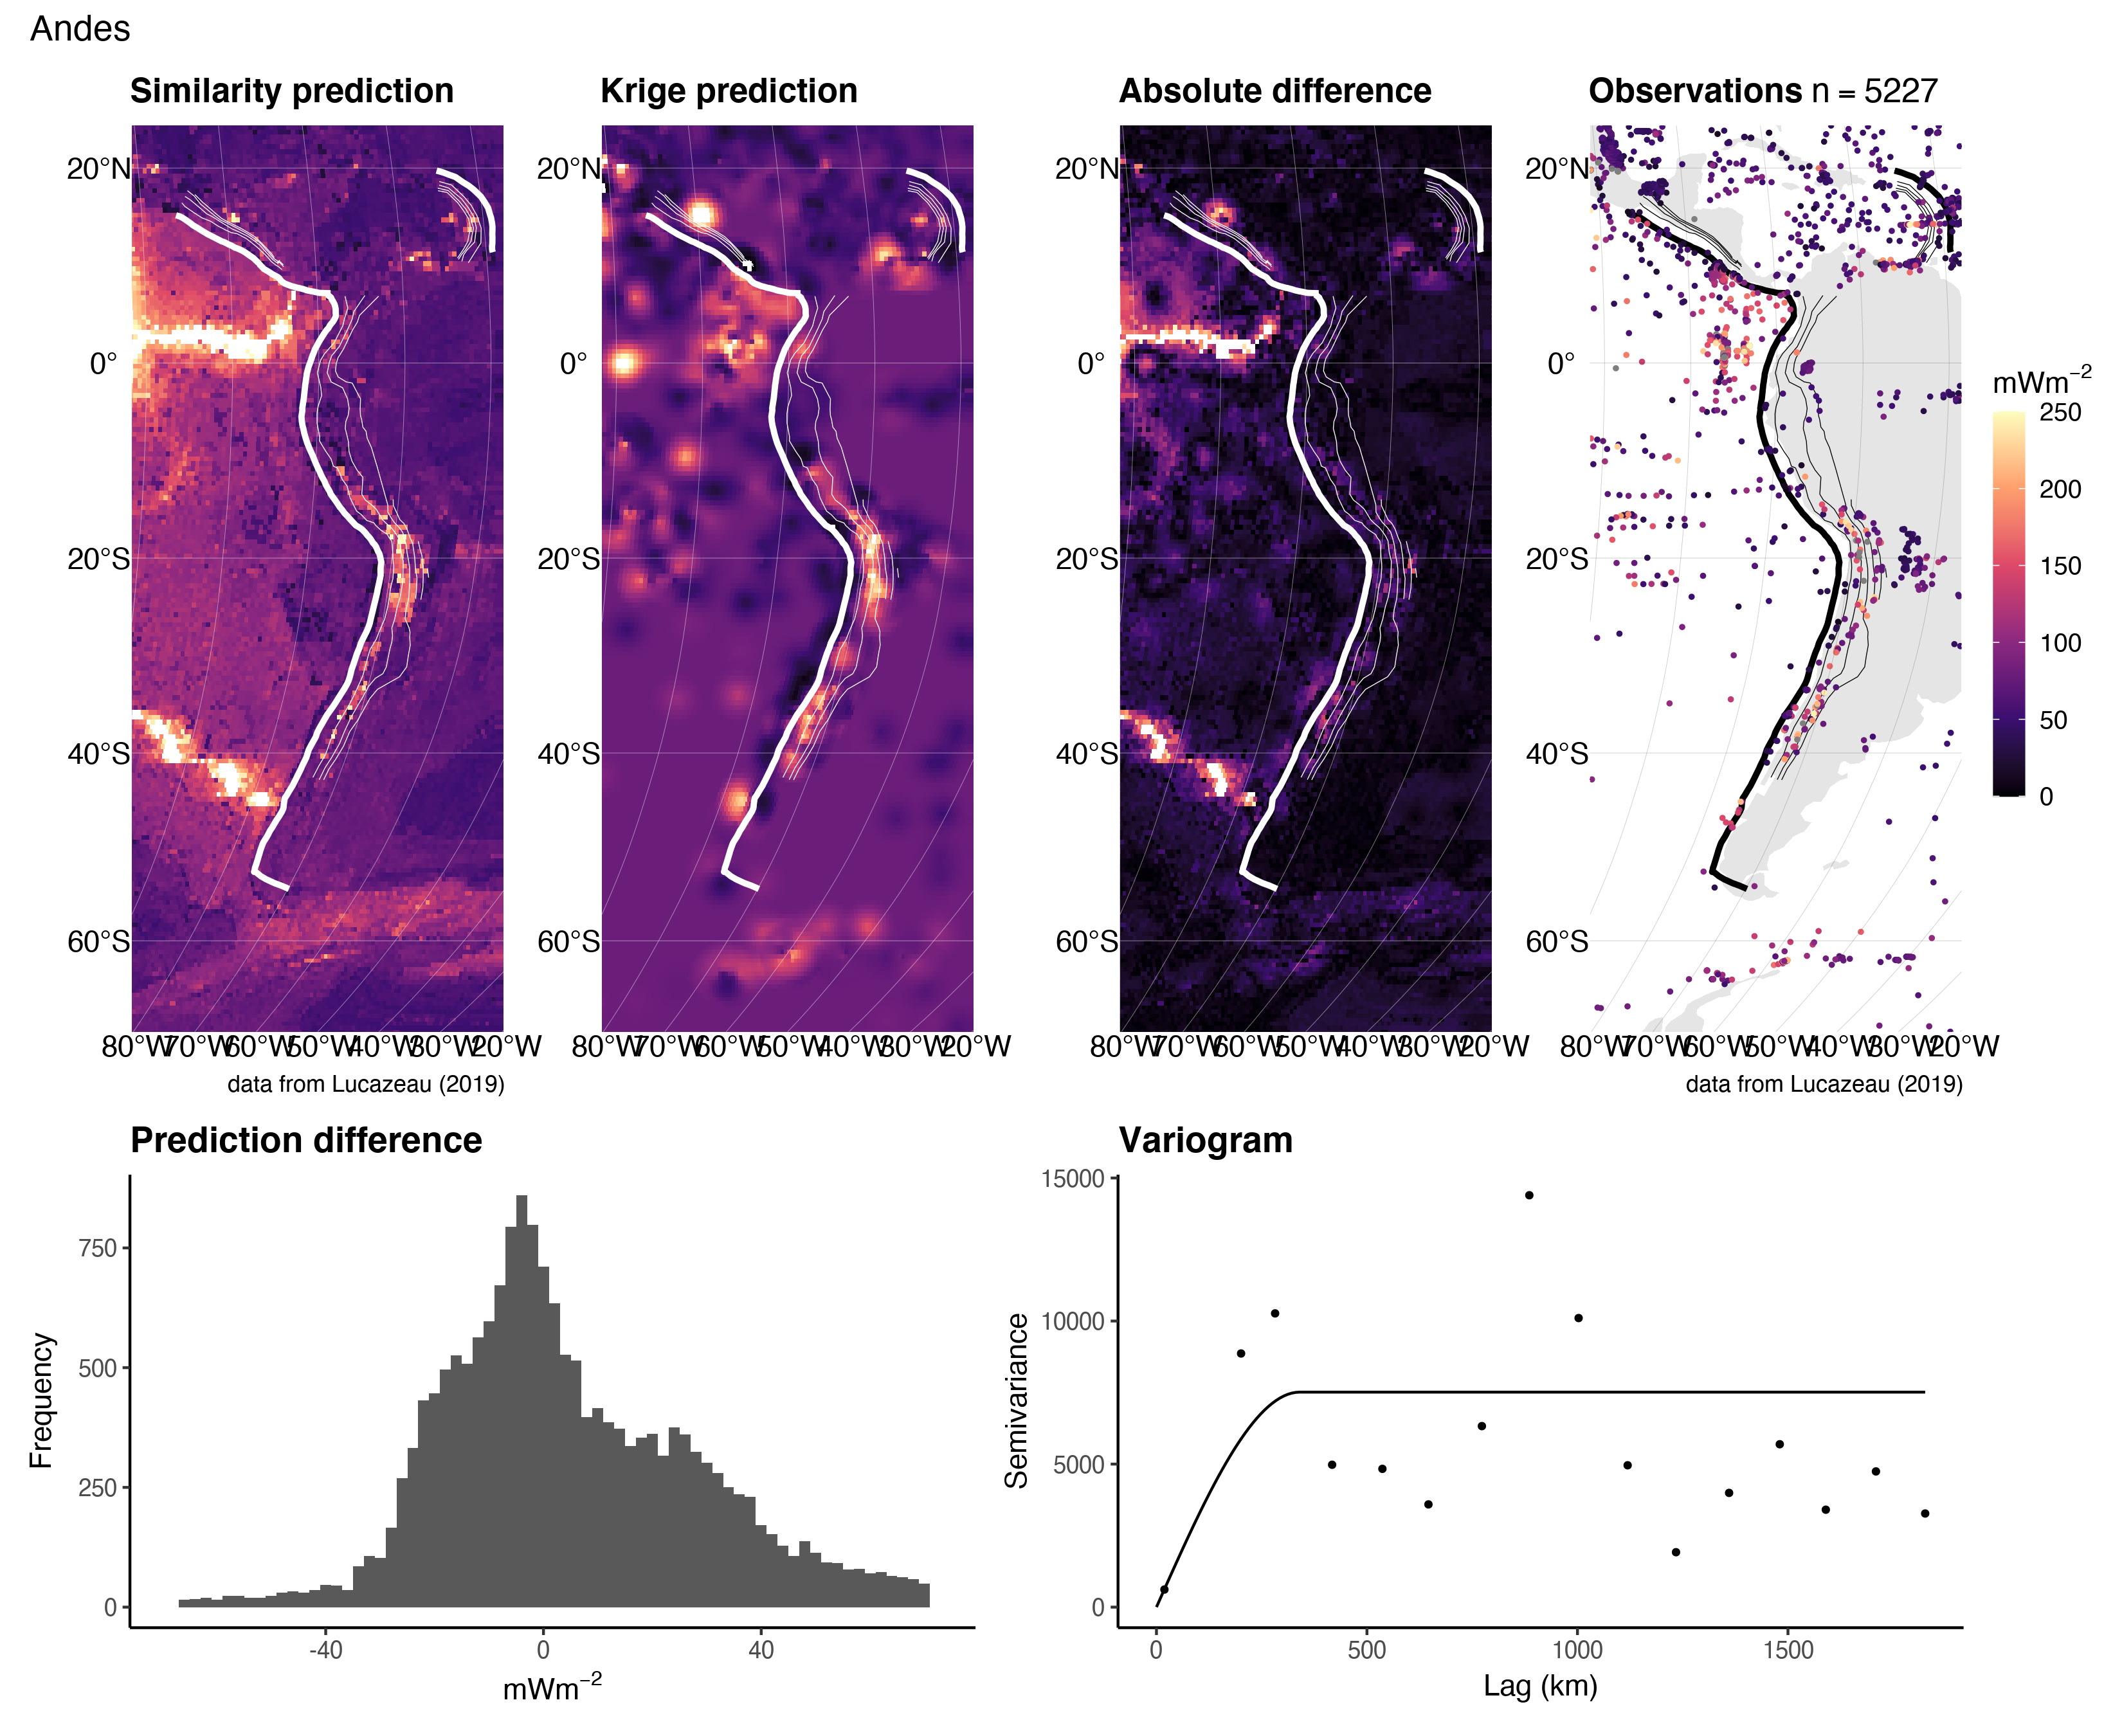
\includegraphics[width=0.95\linewidth,]{../figs/diff/comp/Andes} 

}

\caption{Similarity vs. Kriging predictions for the Andes.}\label{fig:andes.comp}
\end{figure}

\begin{figure}[h]

{\centering 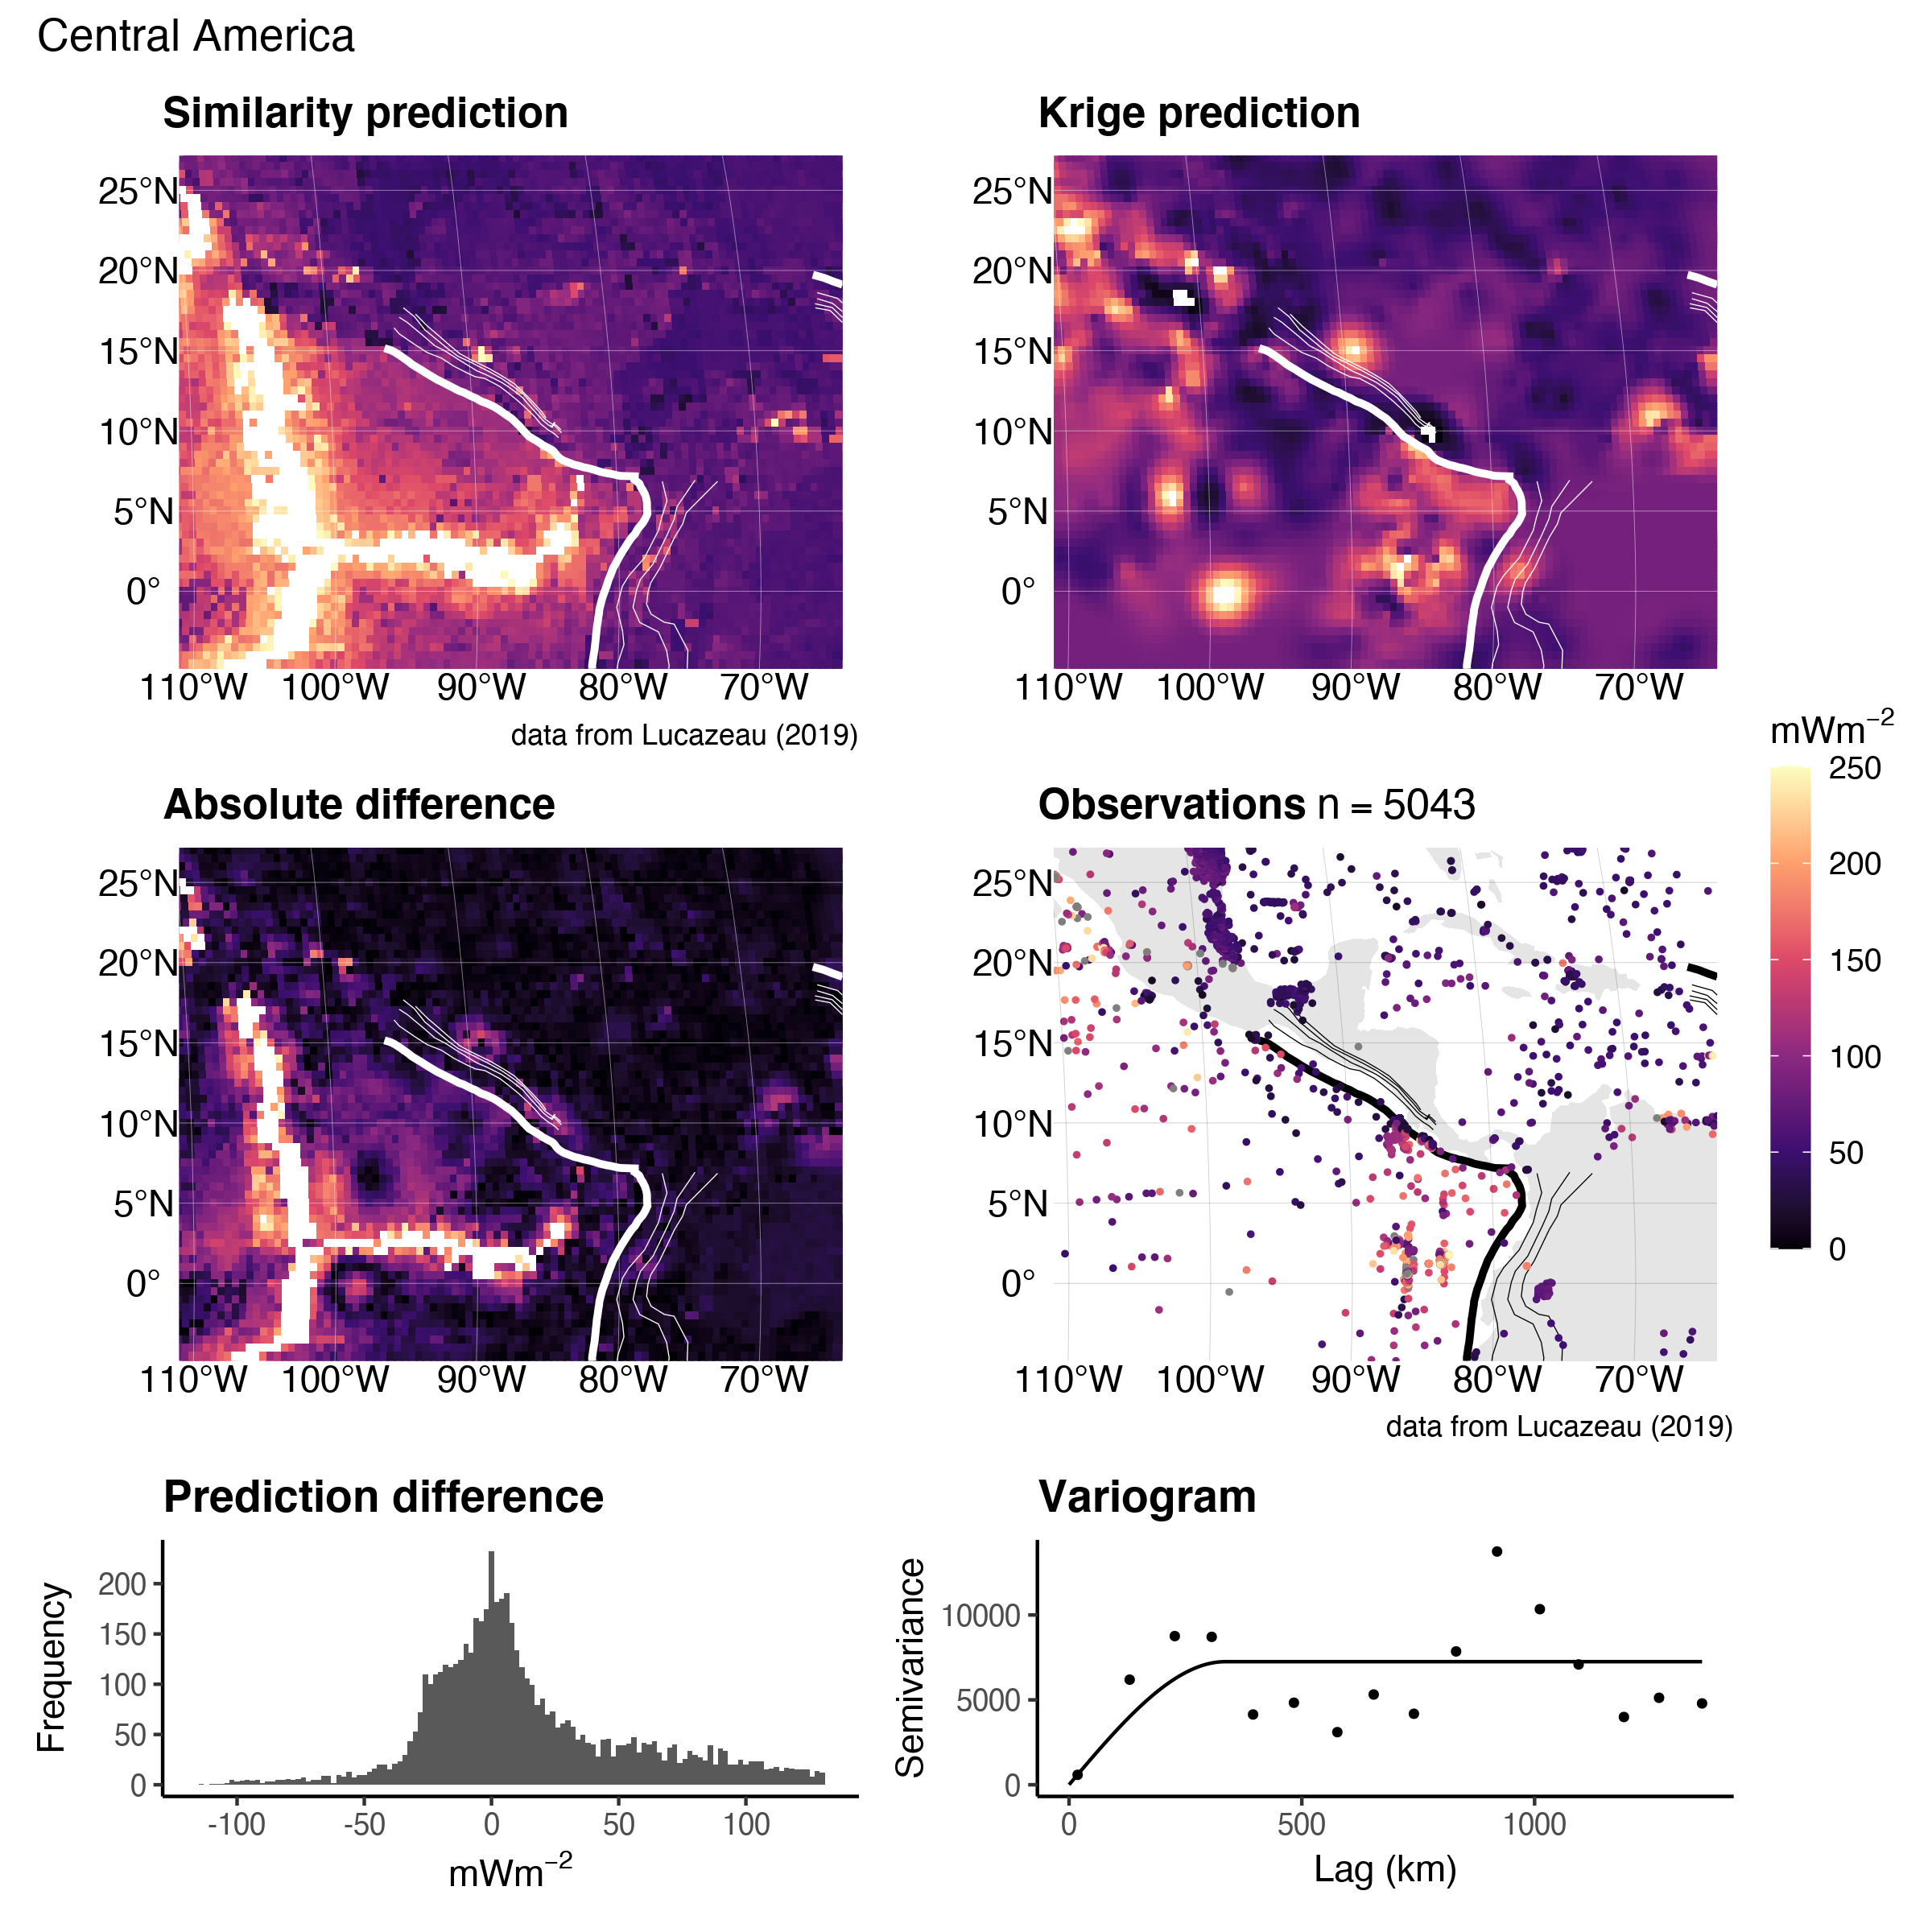
\includegraphics[width=0.95\linewidth,]{../figs/diff/comp/Central_America} 

}

\caption{Similarity vs. Kriging predictions for Central America.}\label{fig:central.america.comp}
\end{figure}

\begin{figure}[h]

{\centering 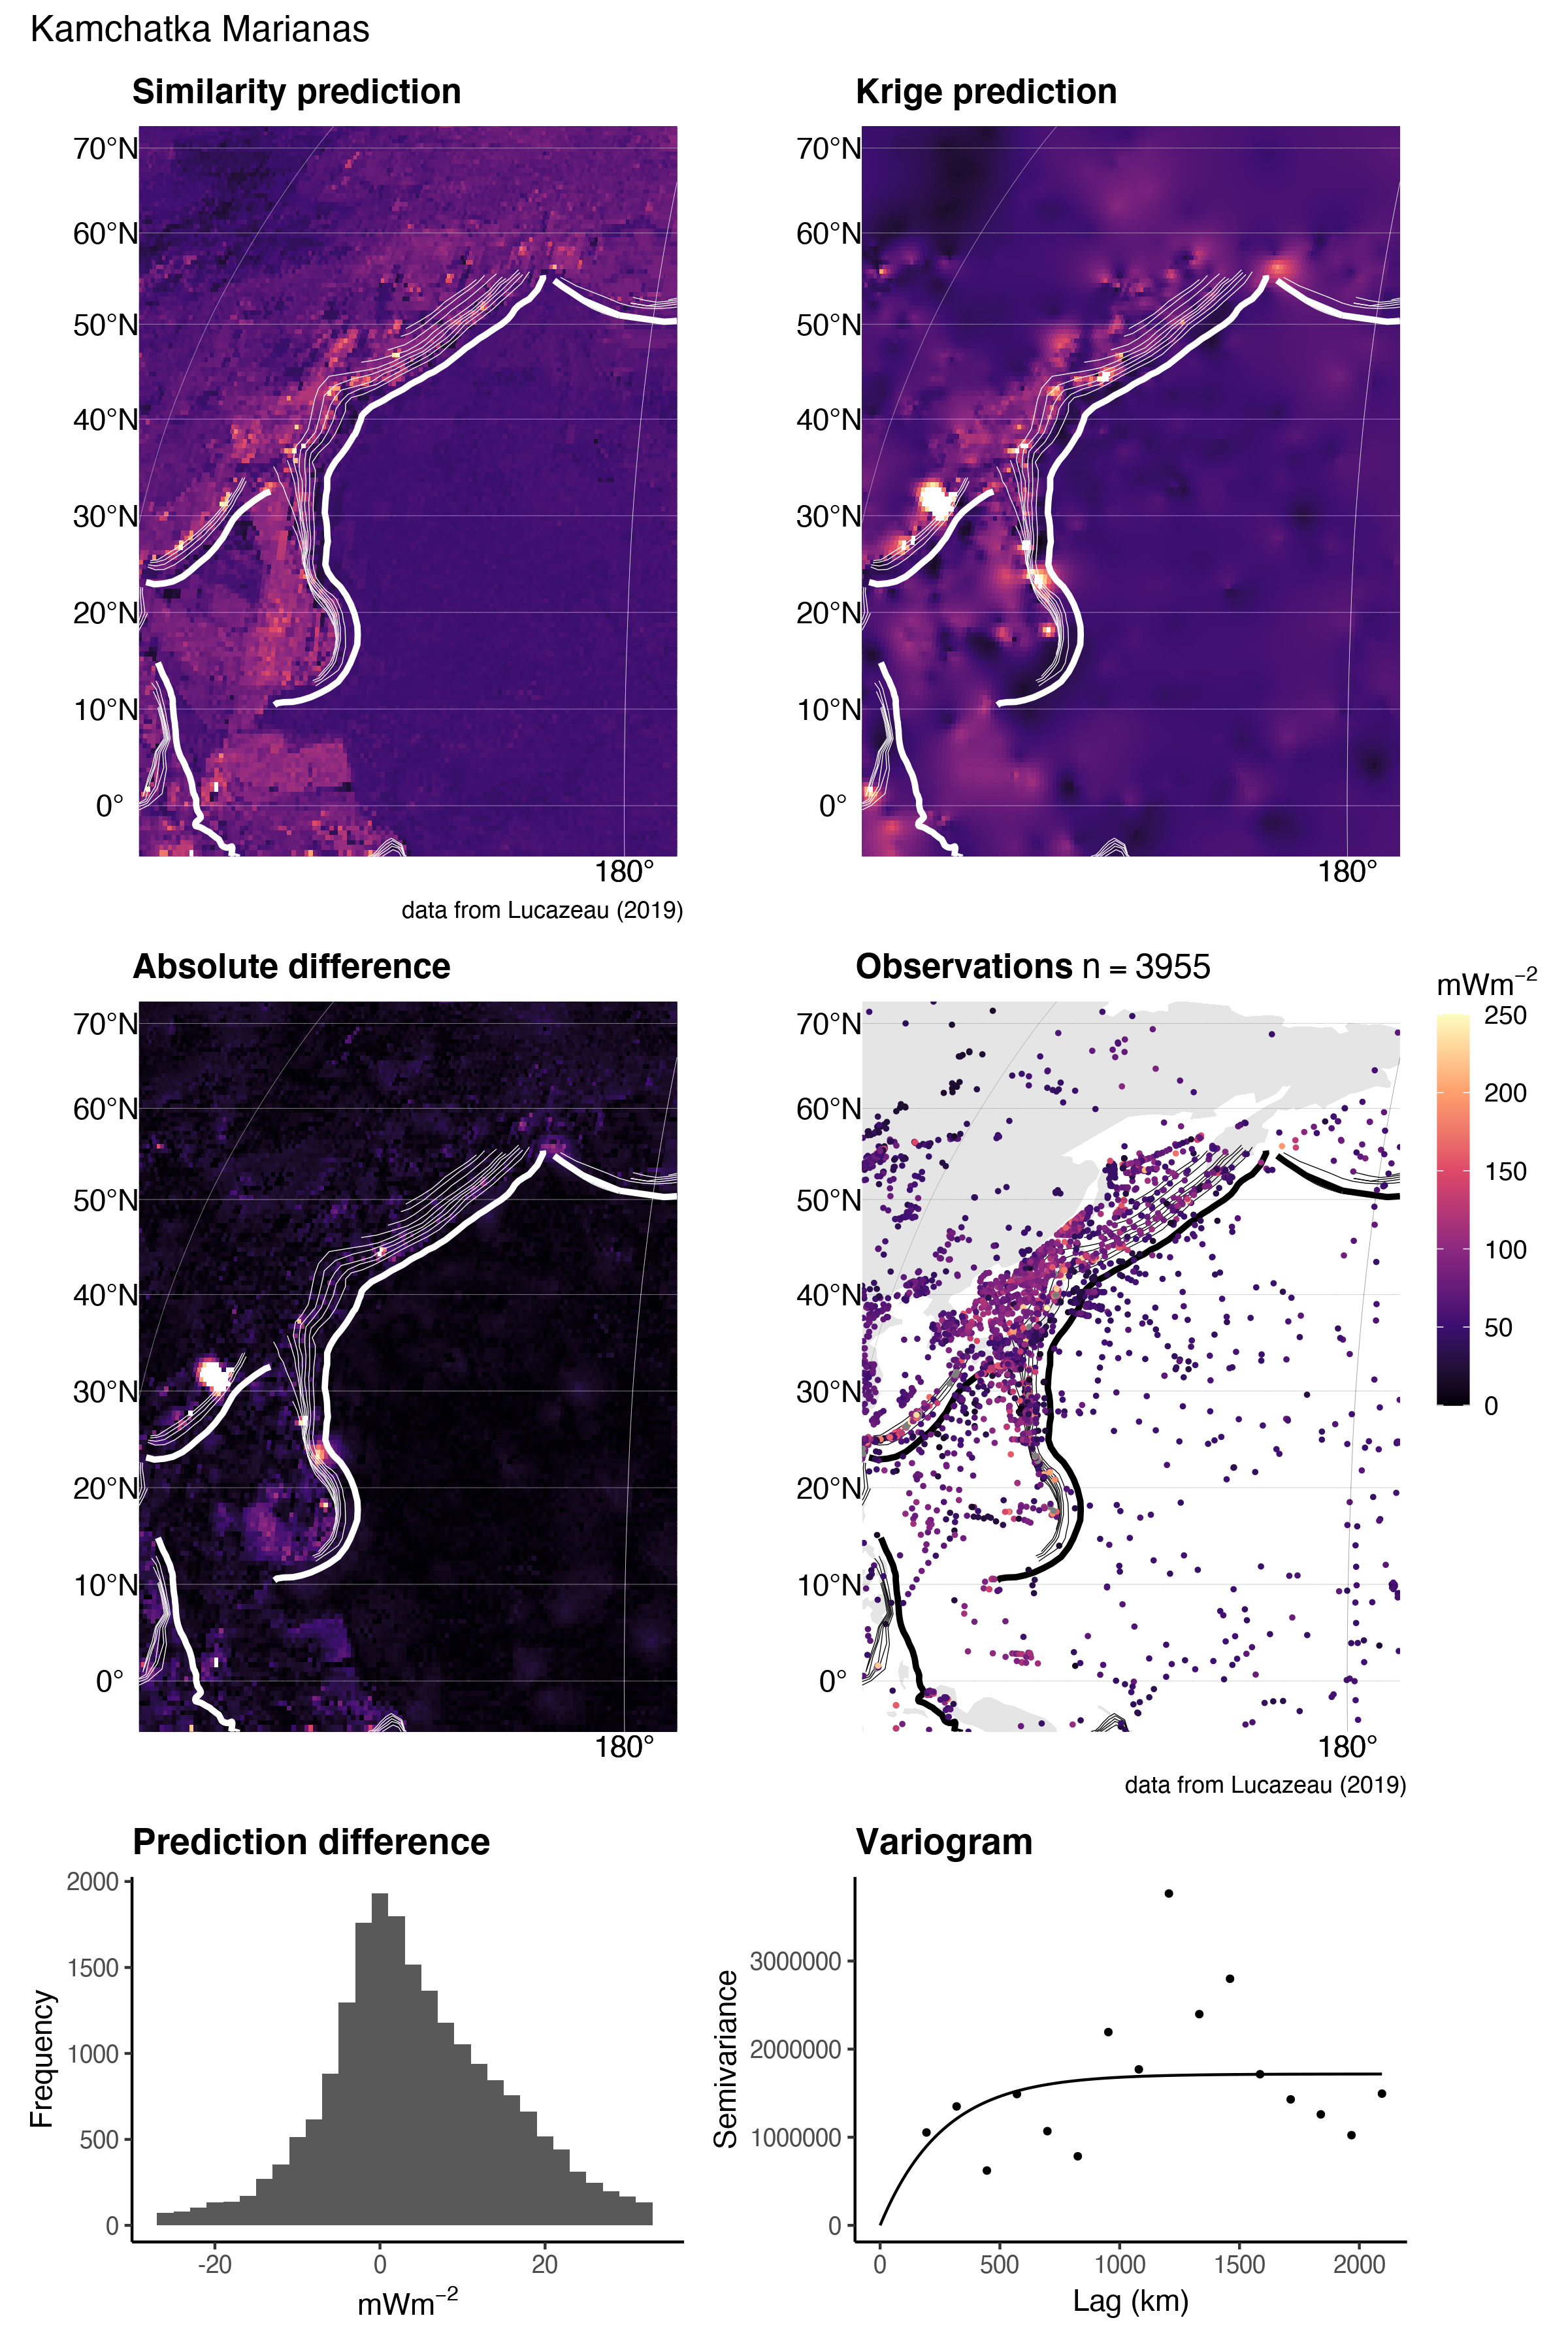
\includegraphics[width=0.95\linewidth,]{../figs/diff/comp/Kamchatka_Marianas} 

}

\caption{Similarity vs. Kriging predictions for Kamchatka Marianas.}\label{fig:kamchatka.marianas.comp}
\end{figure}

\begin{figure}[h]

{\centering 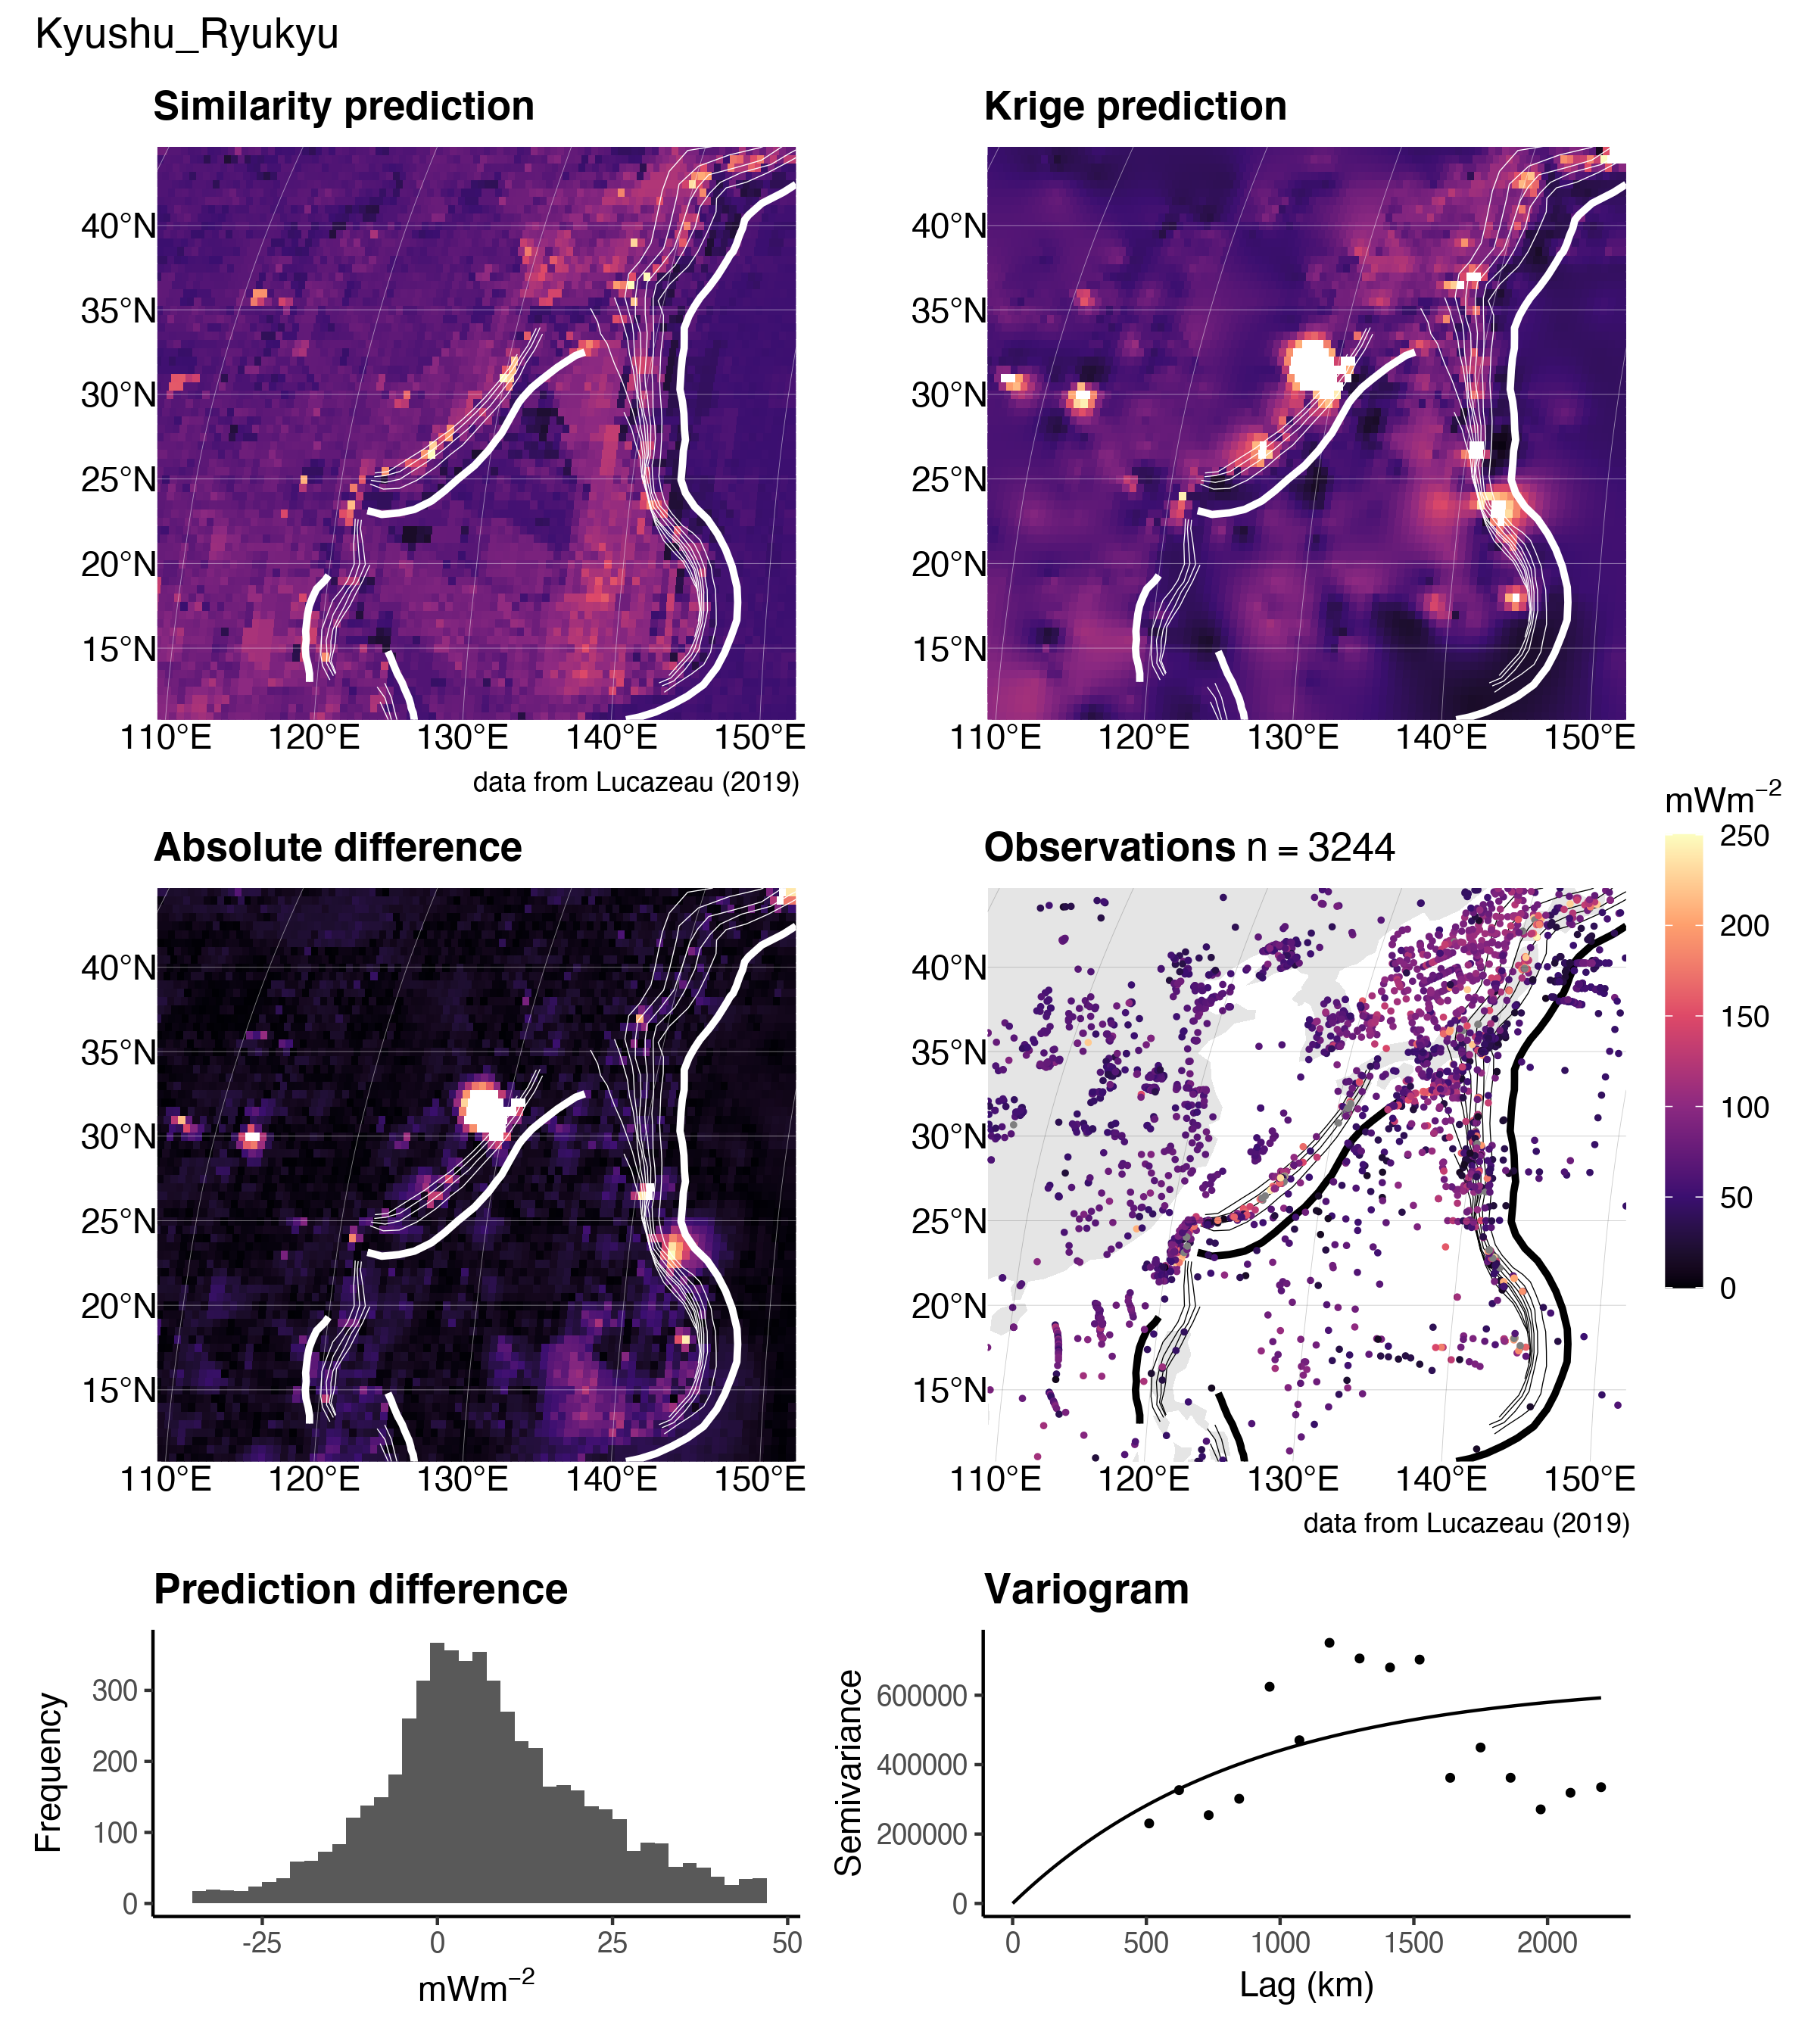
\includegraphics[width=0.95\linewidth,]{../figs/diff/comp/Kyushu_Ryukyu} 

}

\caption{Similarity vs. Kriging predictions for Kyushu Ryukyu.}\label{fig:kyushu.ryukyu.comp}
\end{figure}

\begin{figure}[h]

{\centering 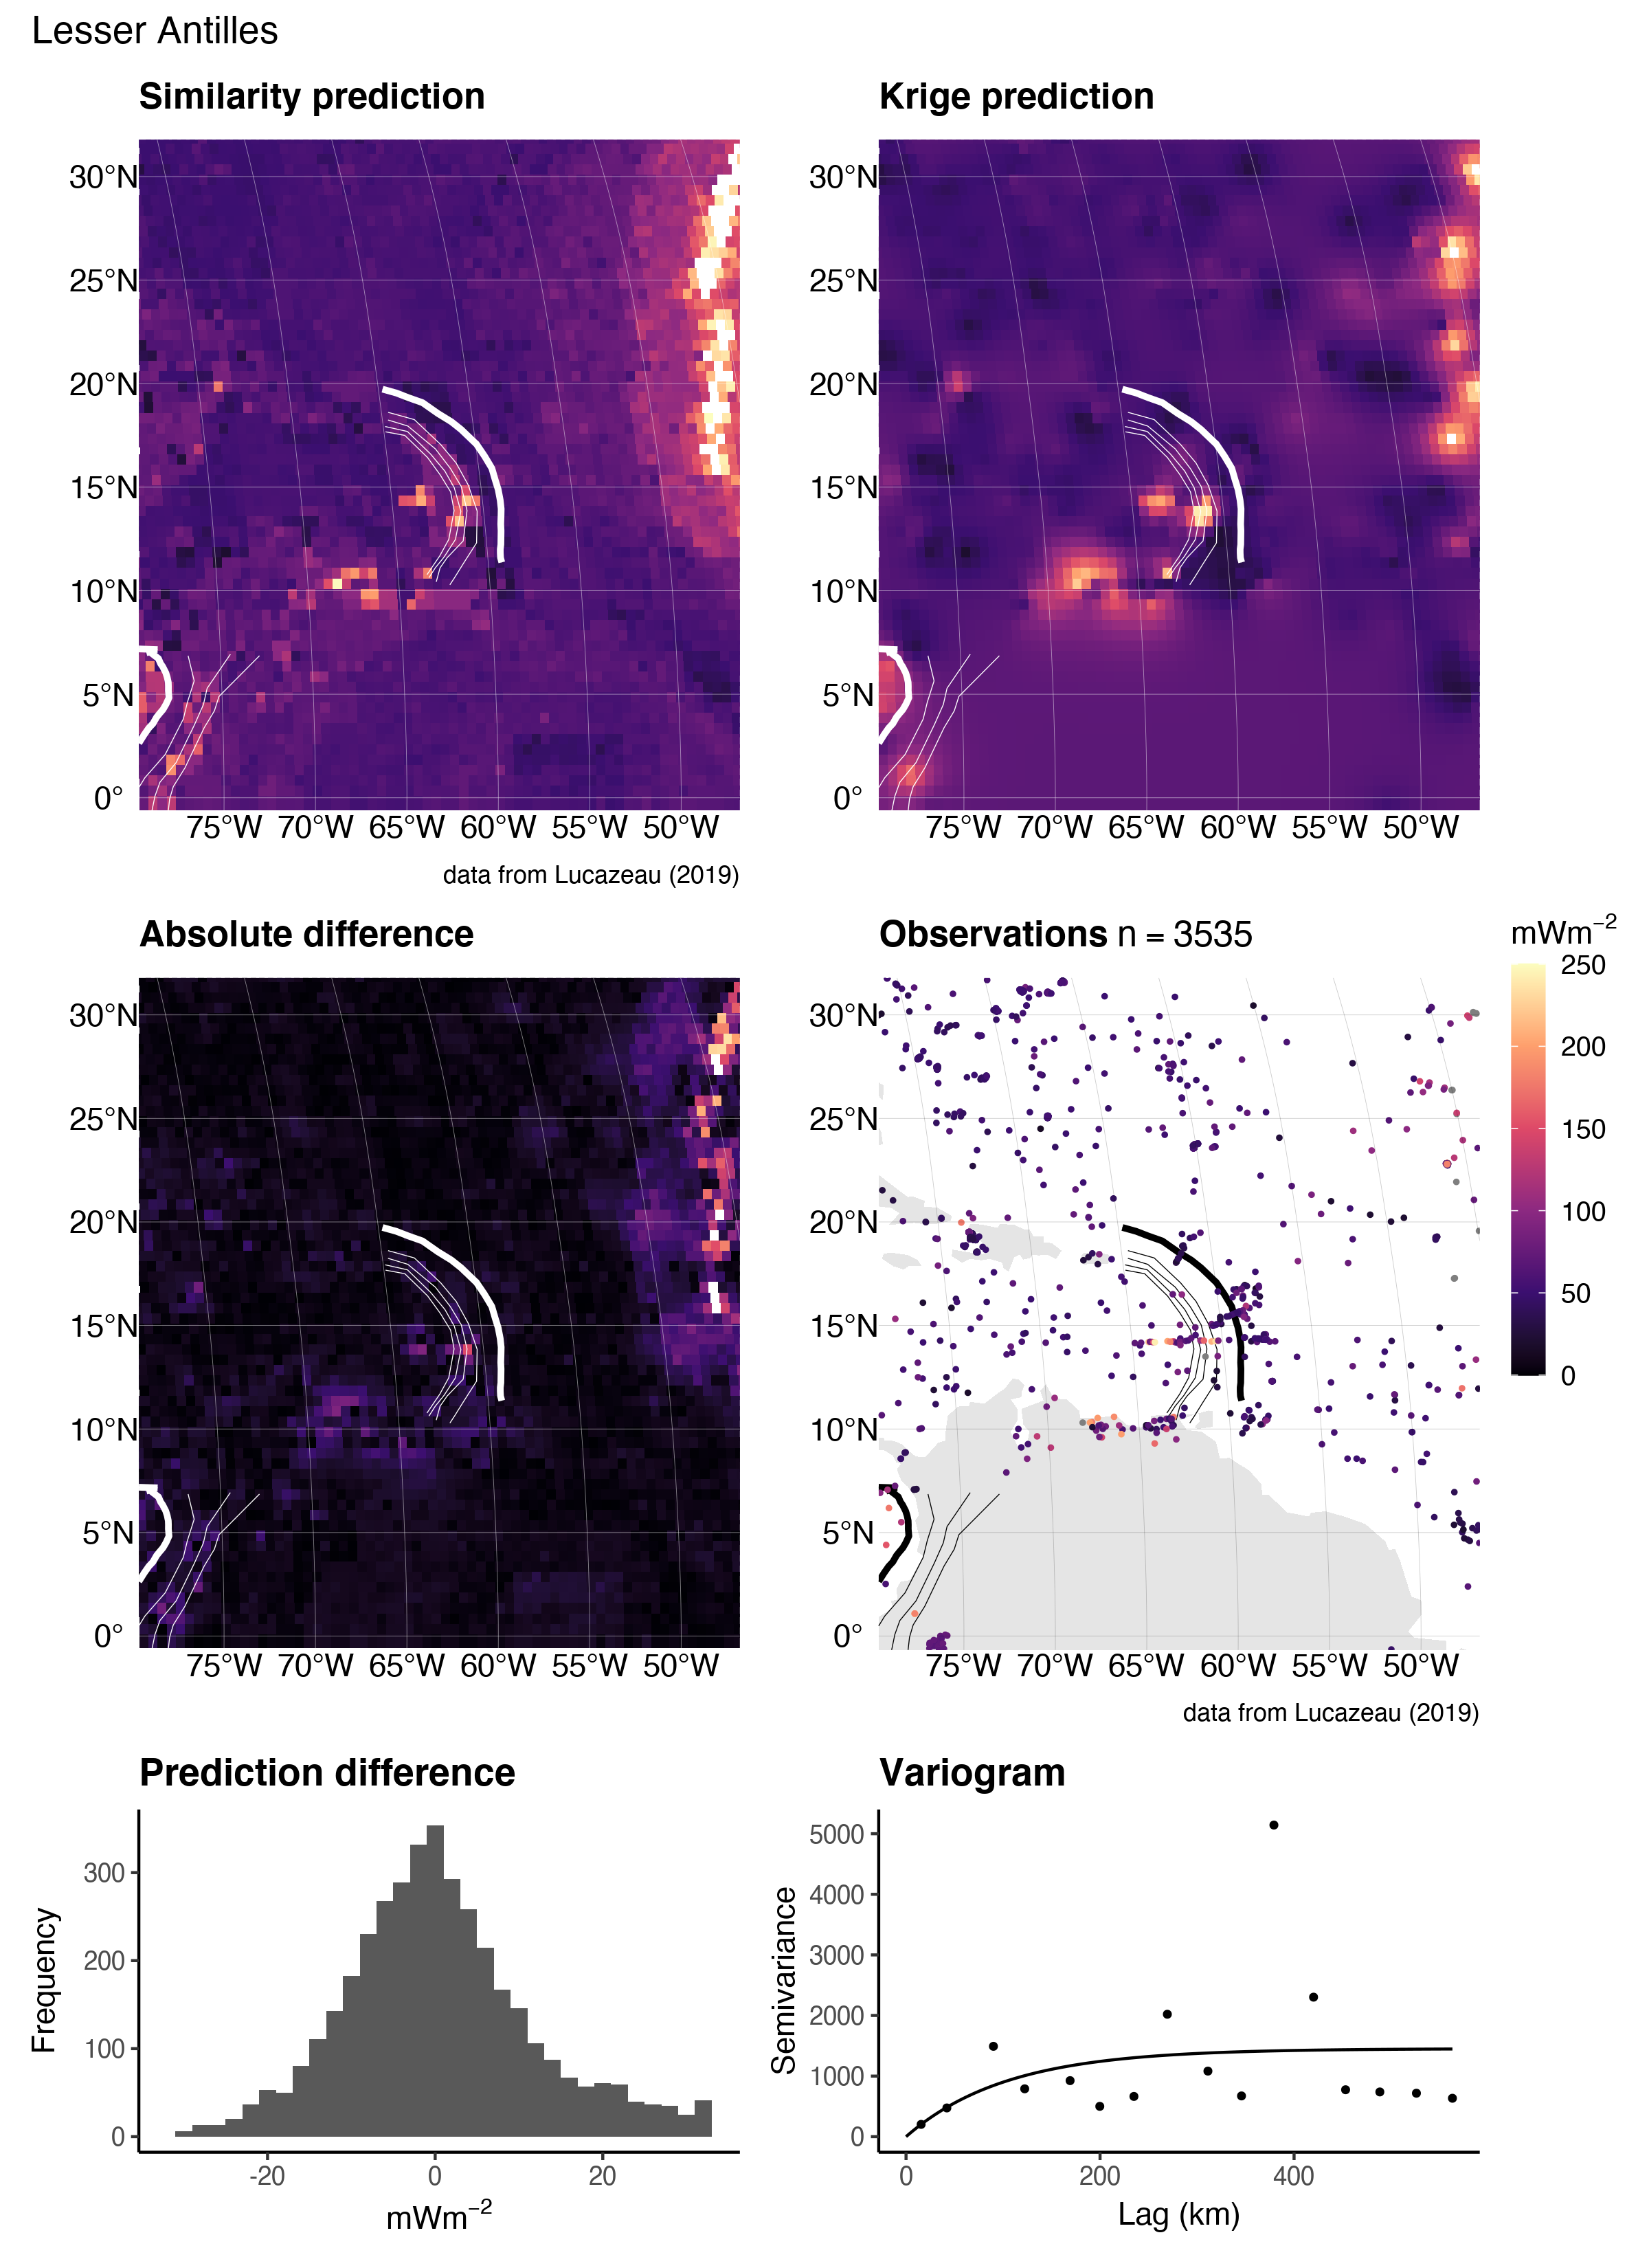
\includegraphics[width=0.95\linewidth,]{../figs/diff/comp/Lesser_Antilles} 

}

\caption{Similarity vs. Kriging predictions for the Lesser Antilles.}\label{fig:lesser.antilles.comp}
\end{figure}

\begin{figure}[h]

{\centering 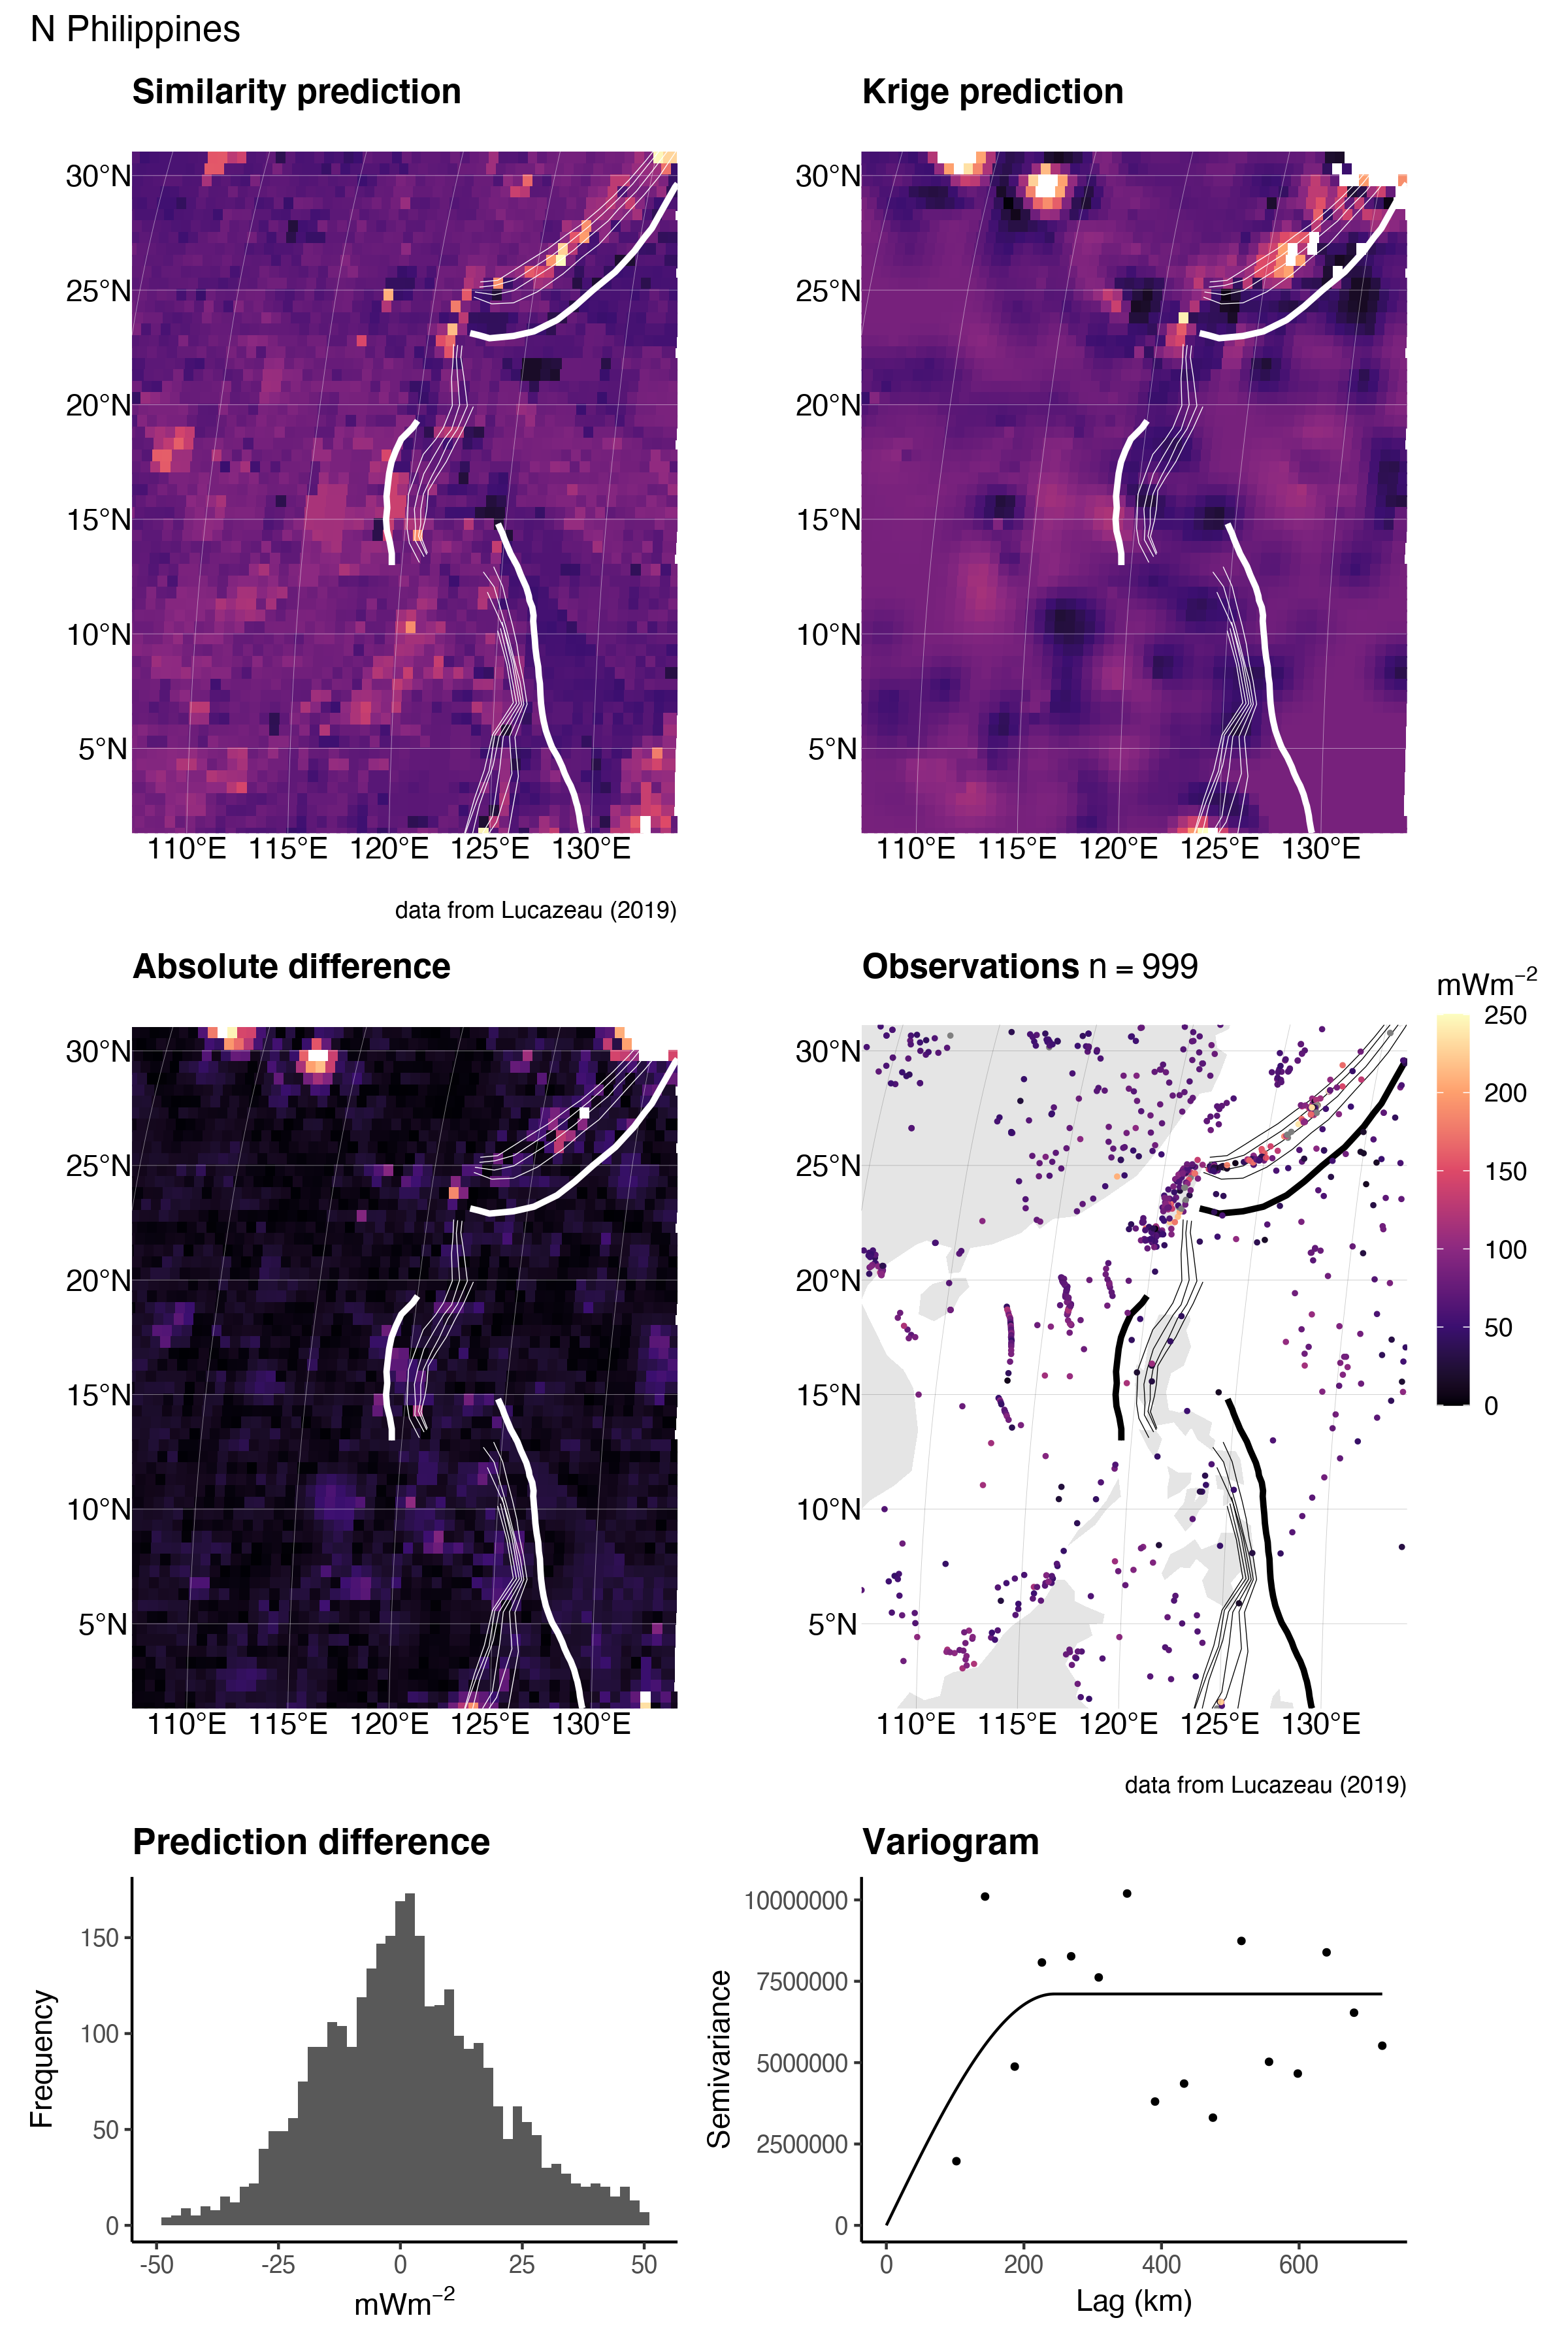
\includegraphics[width=0.95\linewidth,]{../figs/diff/comp/N_Philippines} 

}

\caption{Similarity vs. Kriging predictions for N. Philippines.}\label{fig:n.philippines.comp}
\end{figure}

\begin{figure}[h]

{\centering 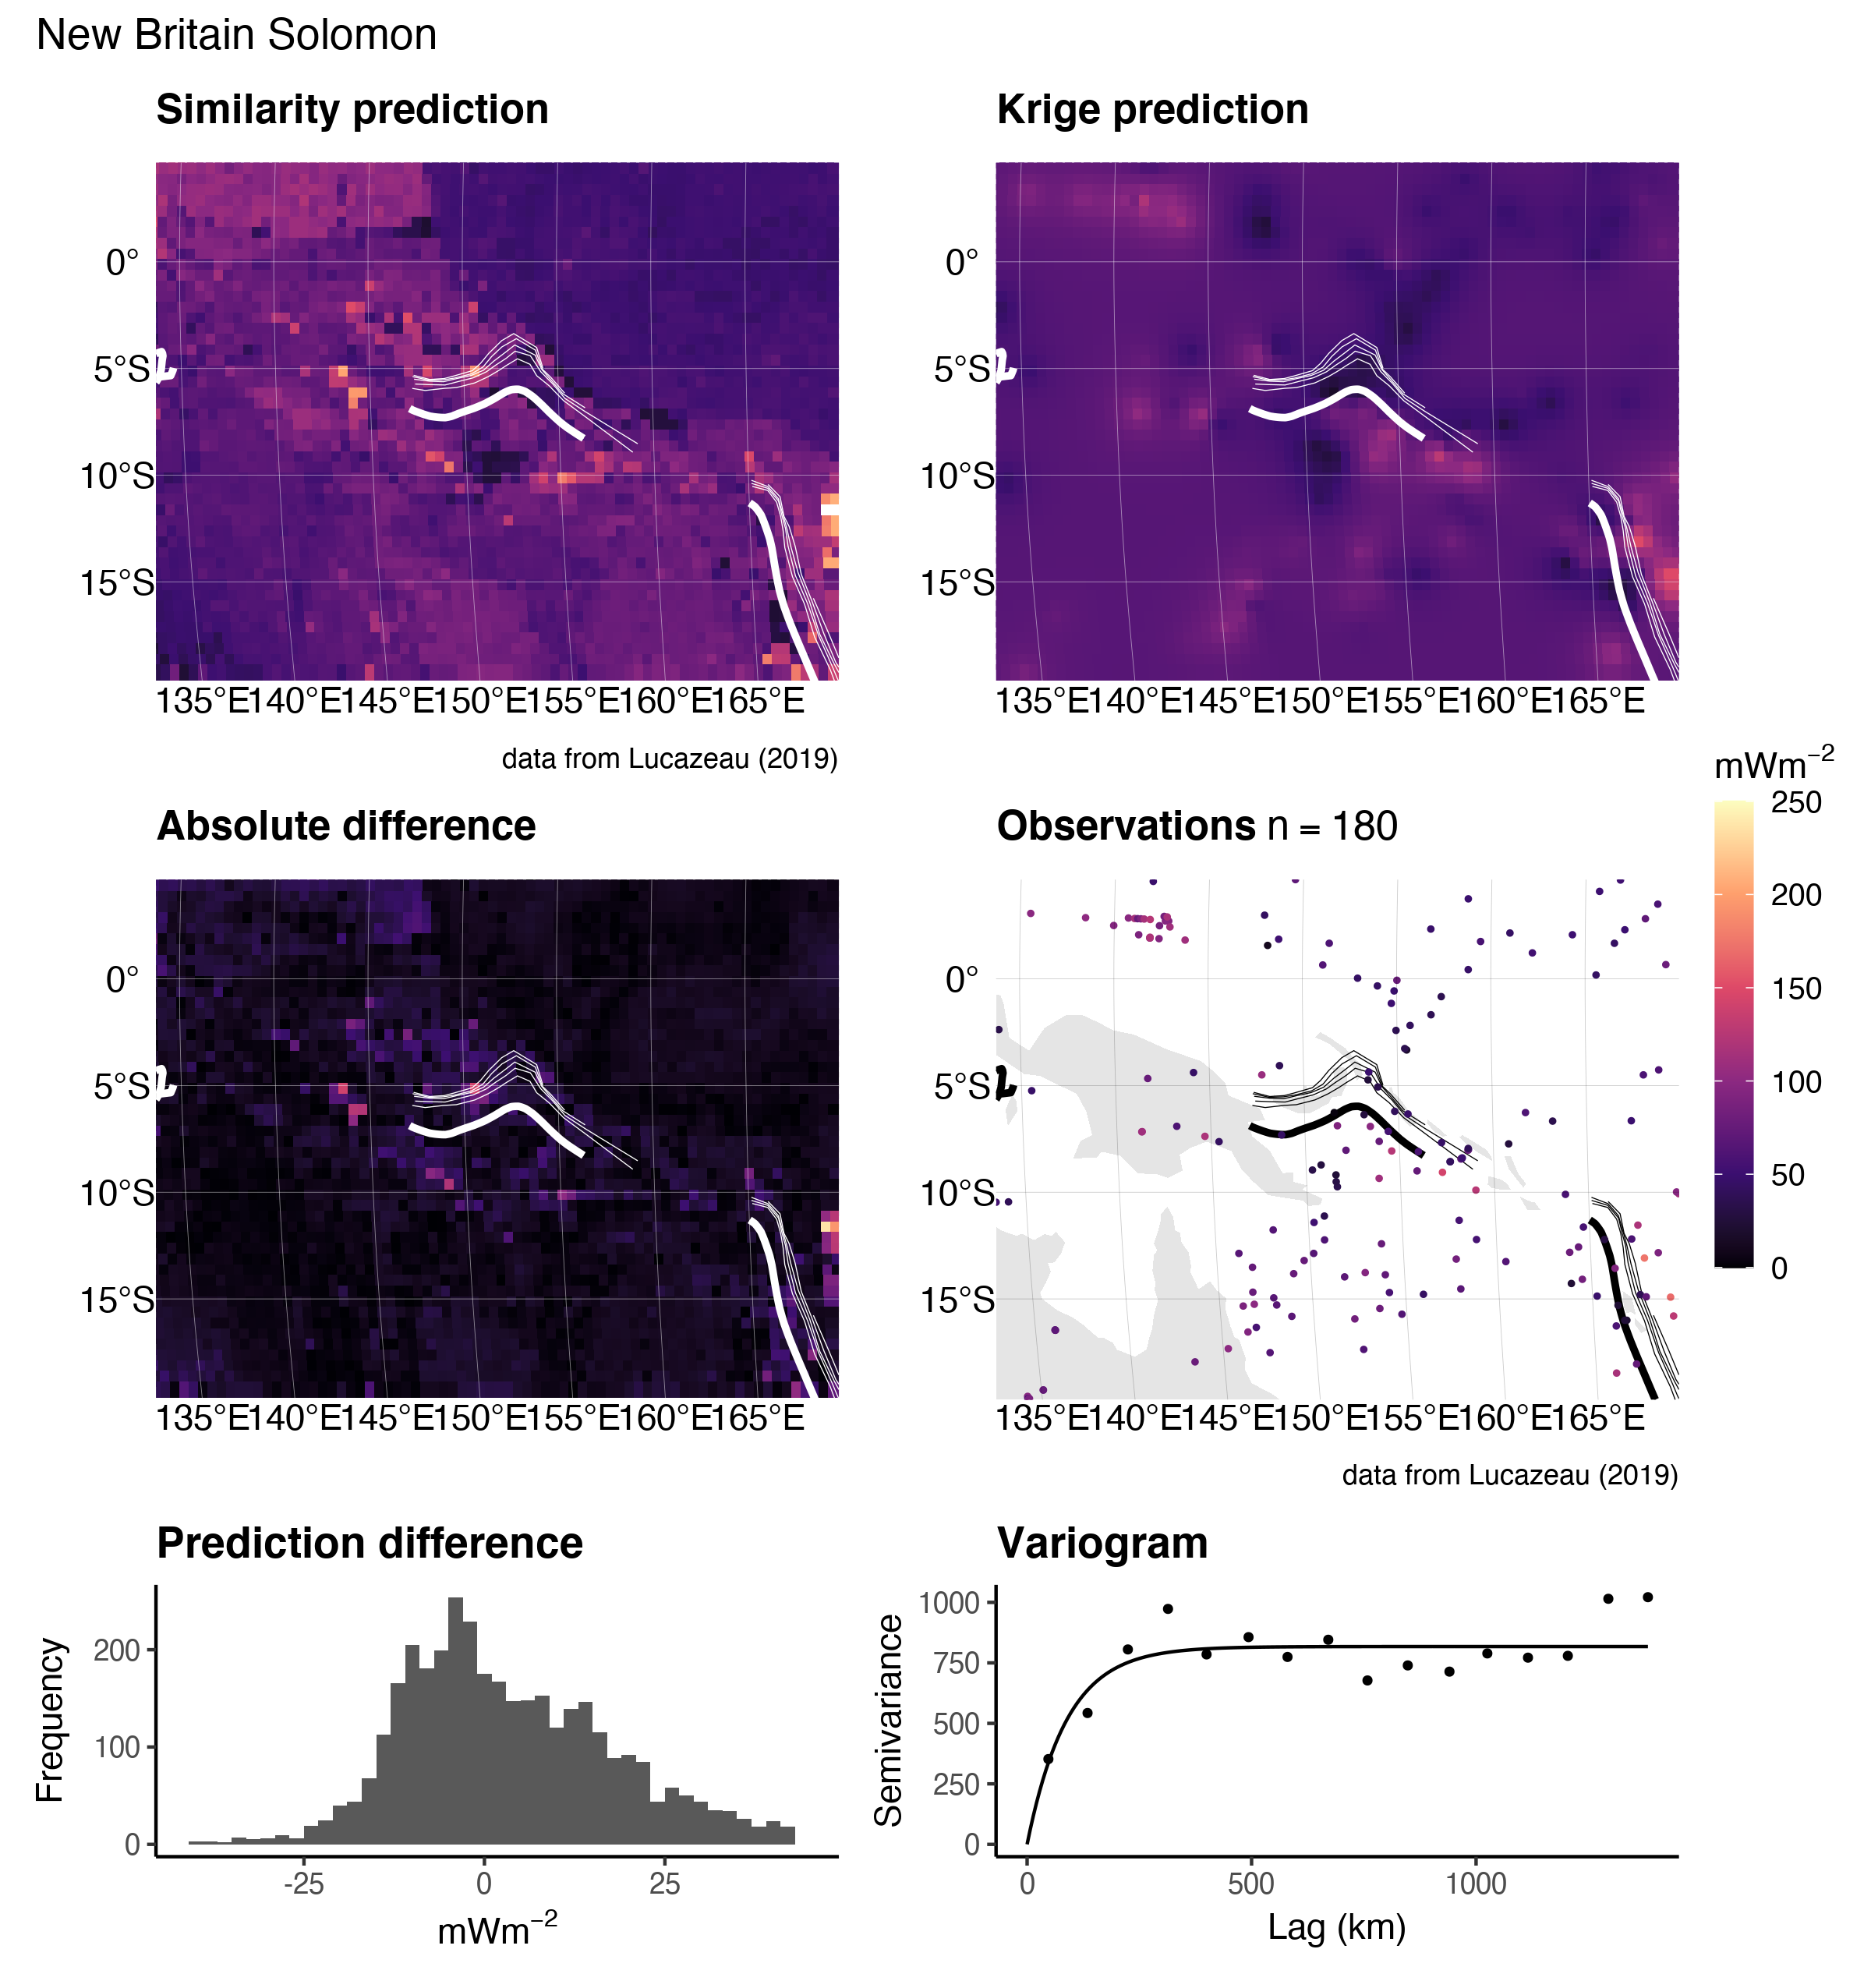
\includegraphics[width=0.95\linewidth,]{../figs/diff/comp/New_Britain_Solomon} 

}

\caption{Similarity vs. Kriging predictions for New Britain Solomon.}\label{fig:new.britain.solomon.comp}
\end{figure}

\begin{figure}[h]

{\centering 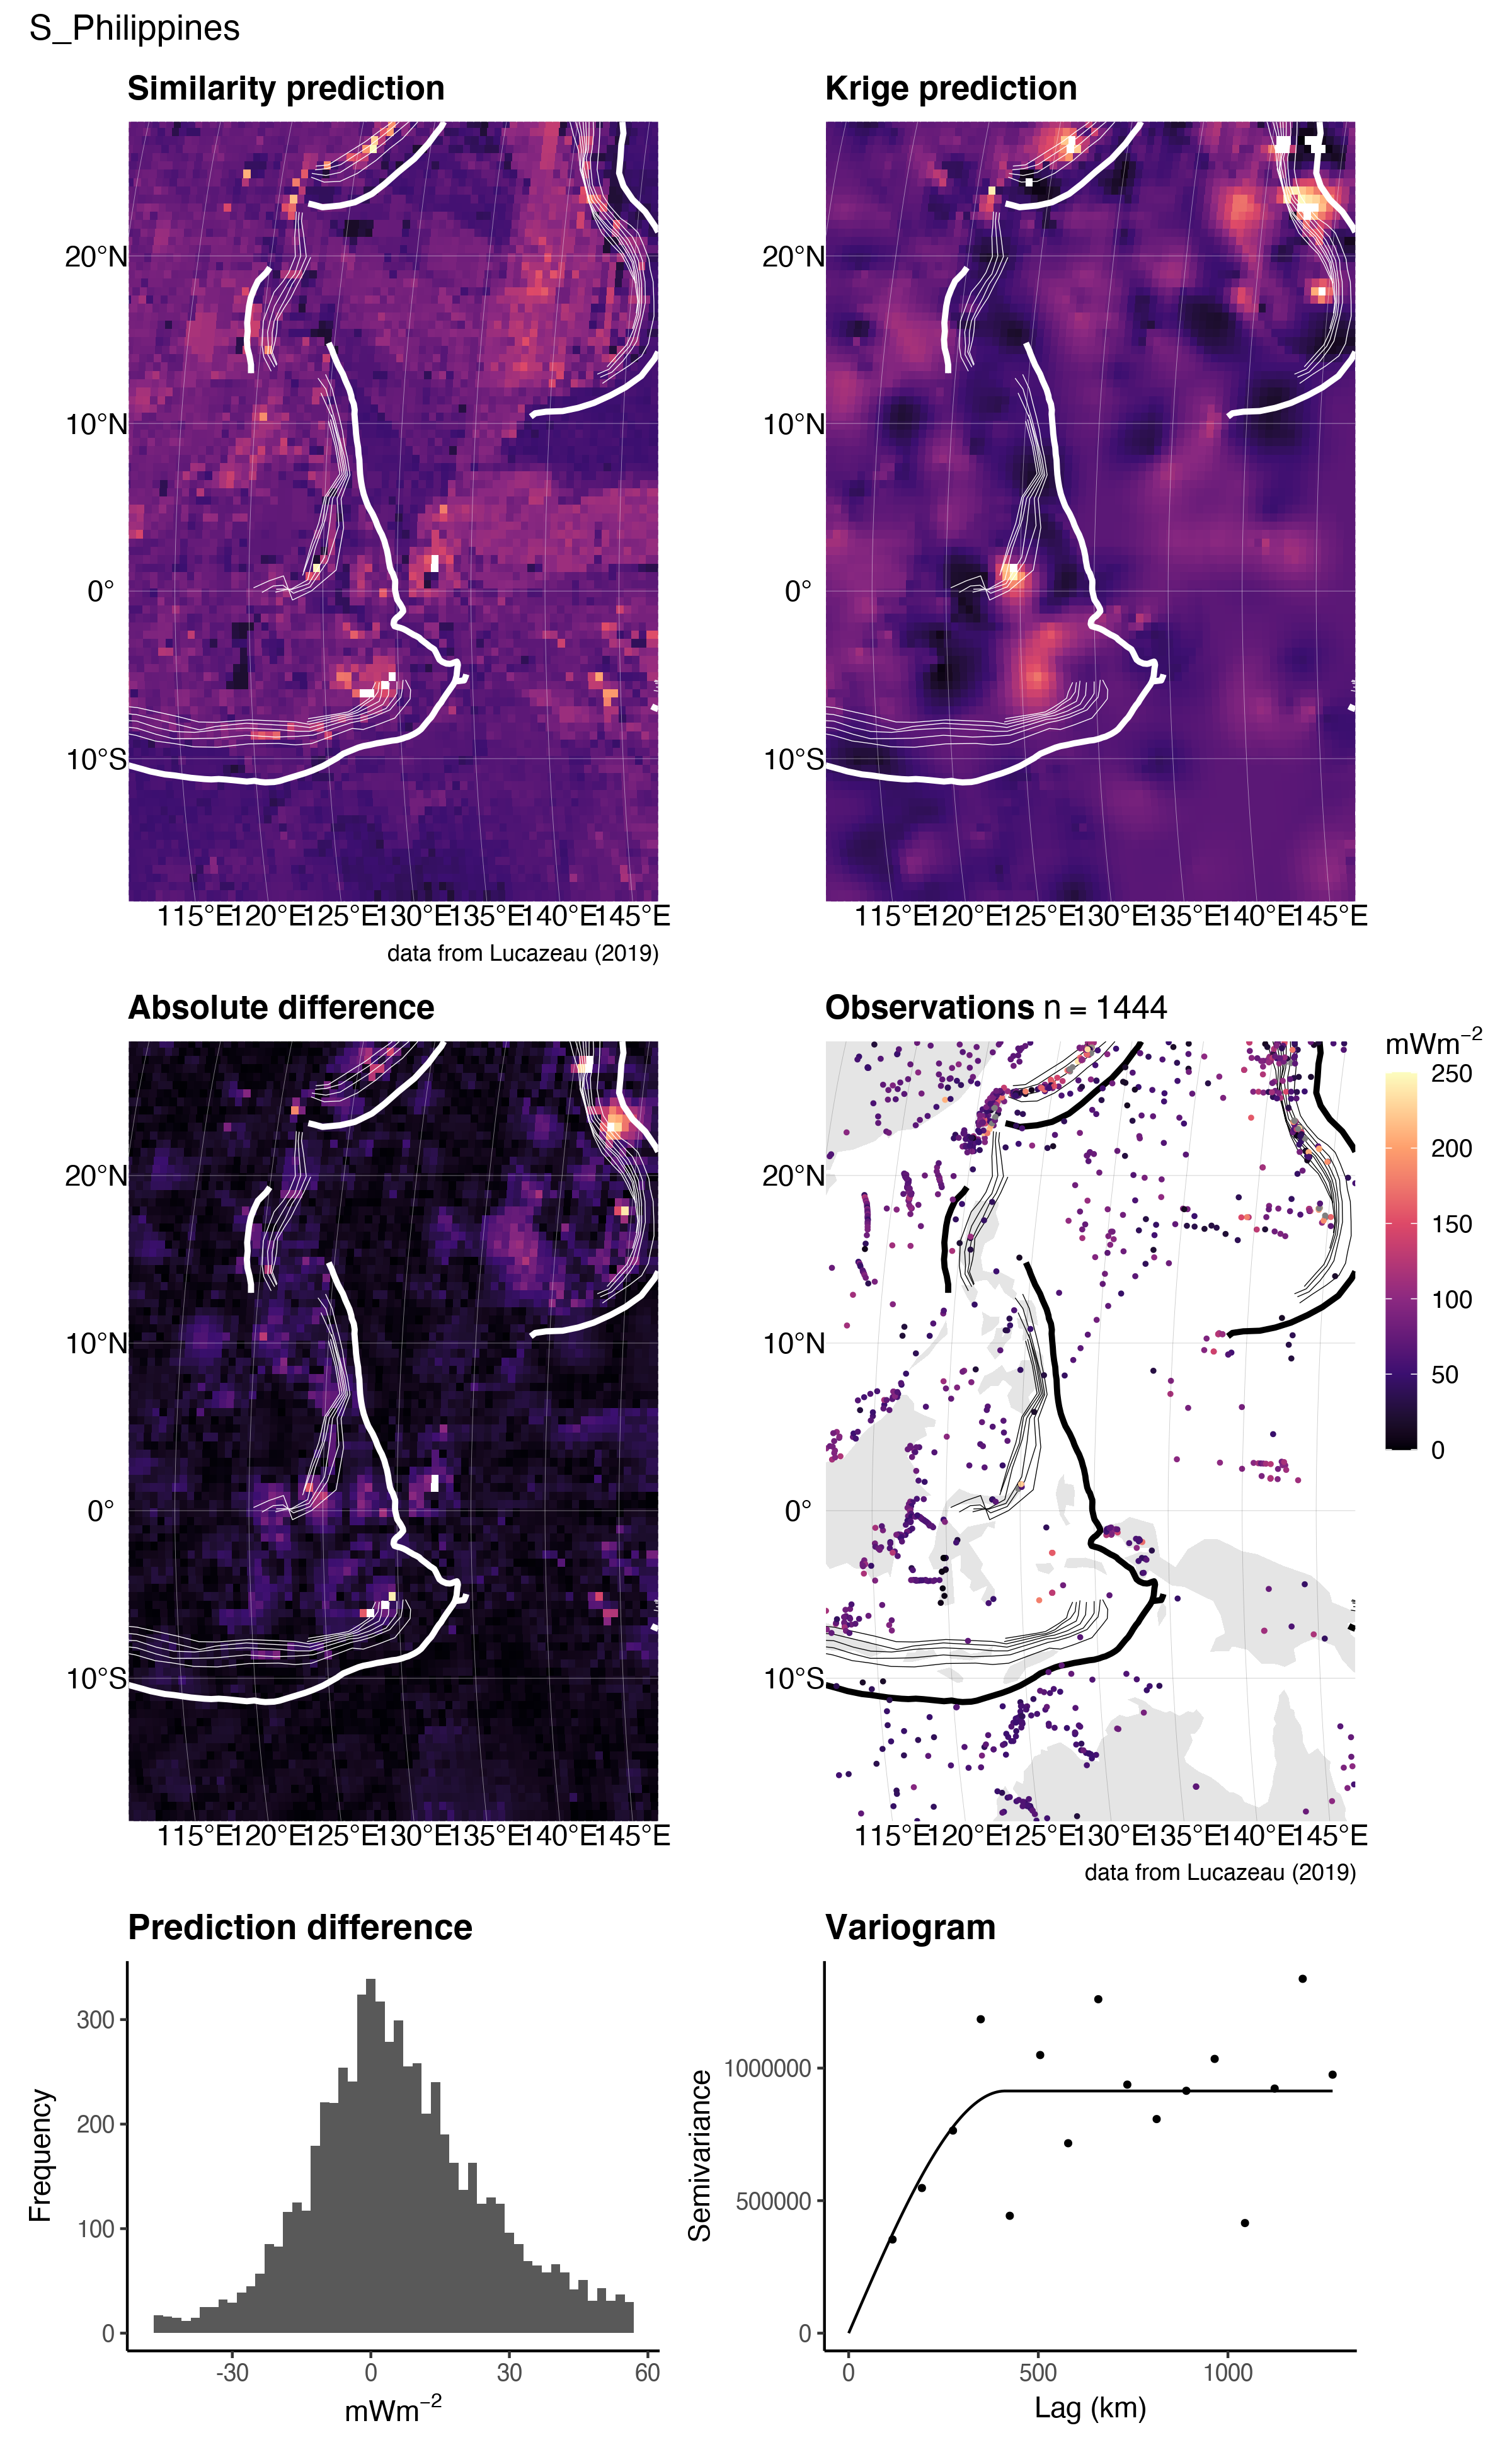
\includegraphics[width=0.95\linewidth,]{../figs/diff/comp/S_Philippines} 

}

\caption{Similarity vs. Kriging predictions for S. Philippines.}\label{fig:s.philippines.comp}
\end{figure}

\begin{figure}[h]

{\centering 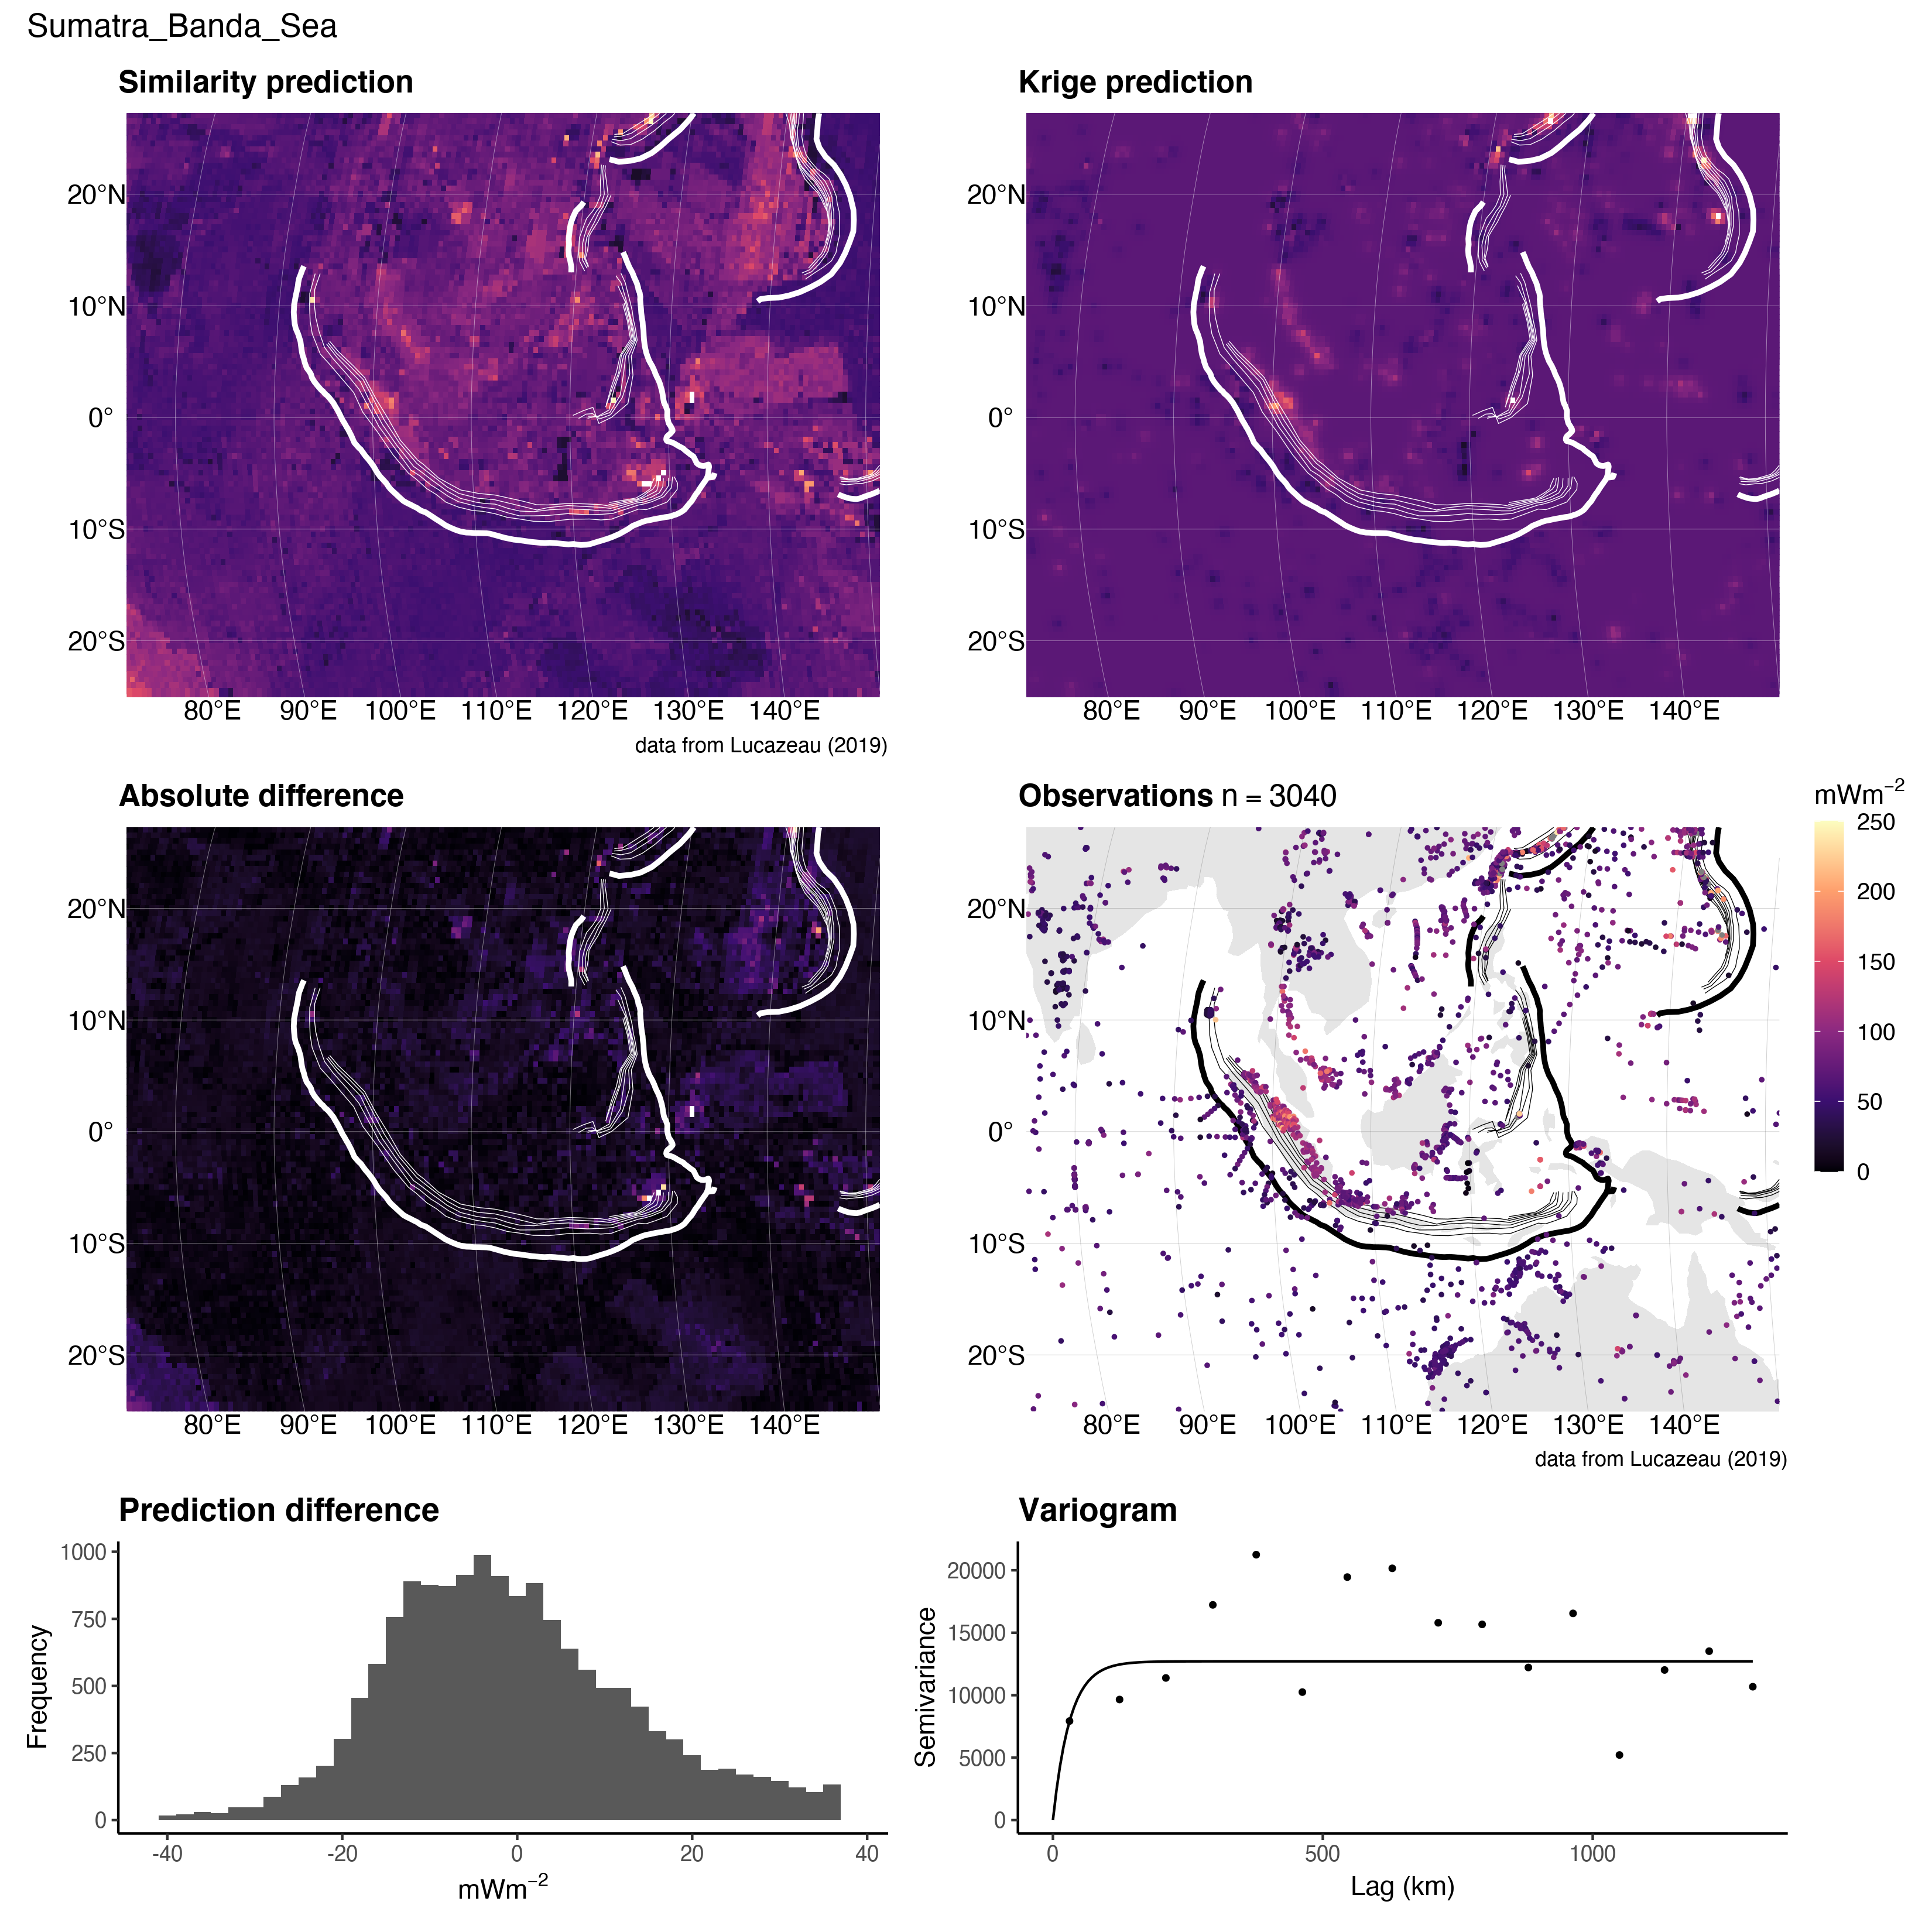
\includegraphics[width=0.95\linewidth,]{../figs/diff/comp/Sumatra_Banda_Sea} 

}

\caption{Similarity vs. Kriging predictions for Sumatra Banda Sea.}\label{fig:sumatra.banda.sea.comp}
\end{figure}

\begin{figure}[h]

{\centering 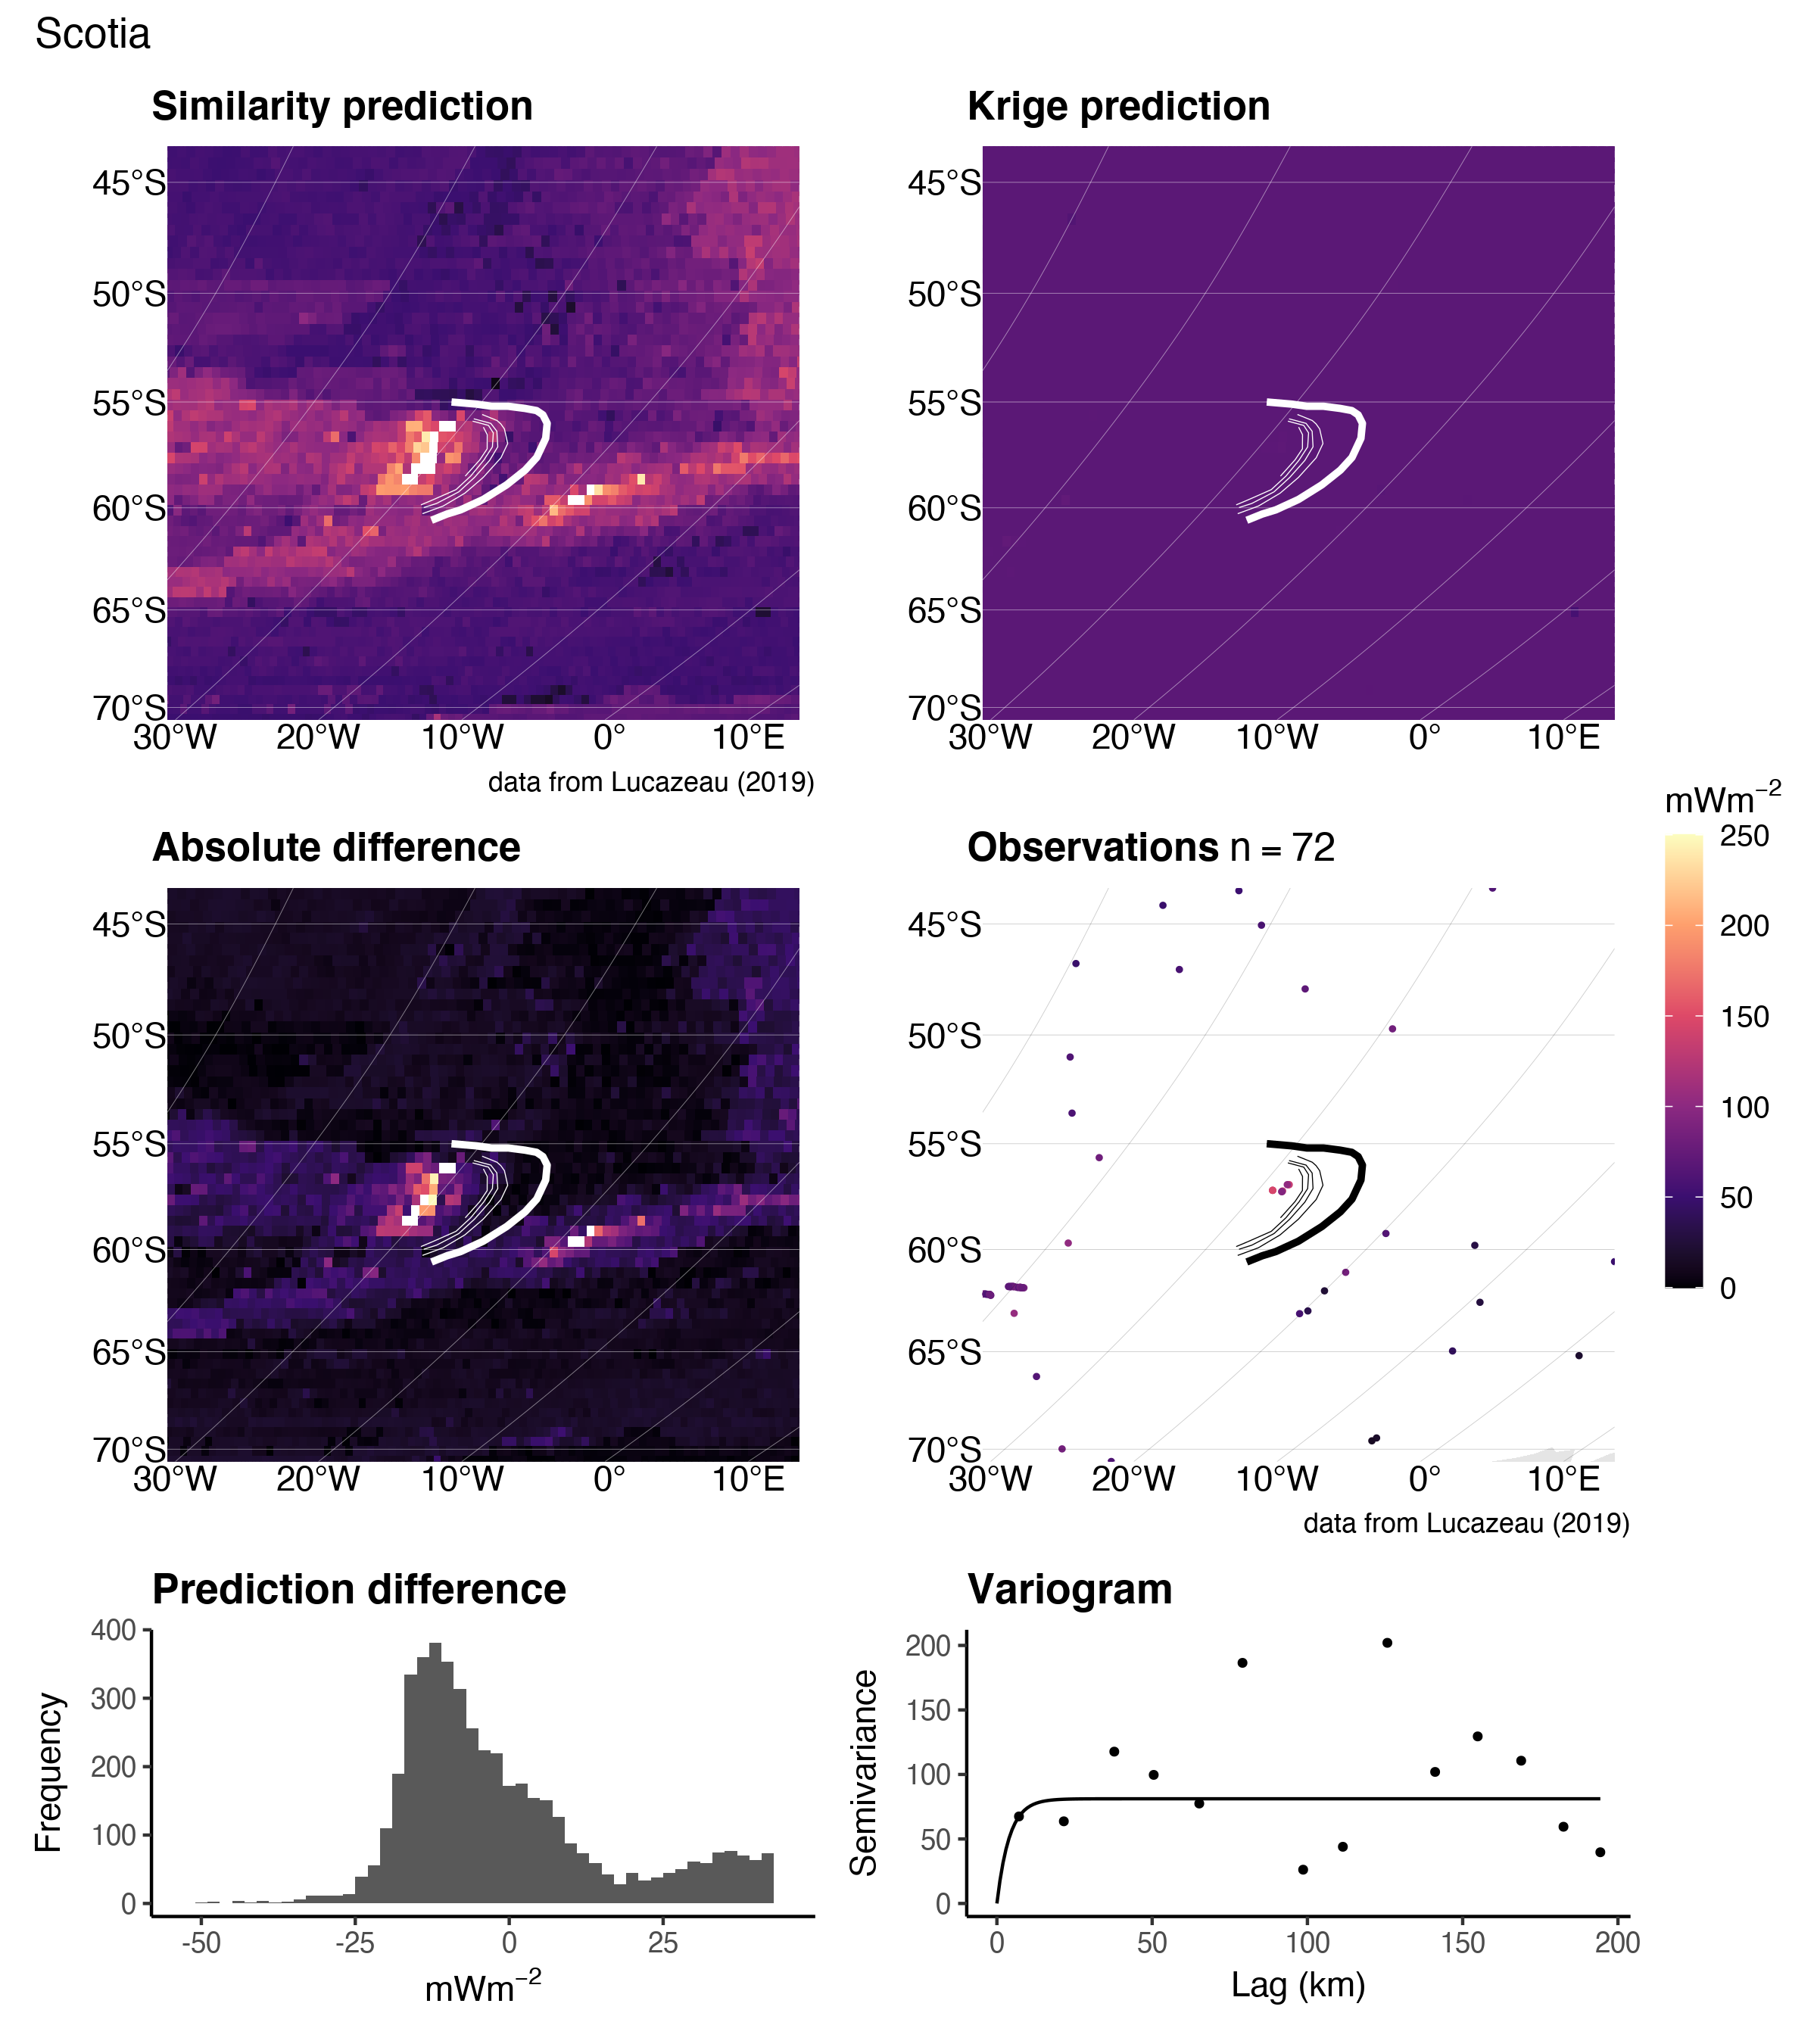
\includegraphics[width=0.95\linewidth,]{../figs/diff/comp/Scotia} 

}

\caption{Similarity vs. Kriging predictions for Scotia.}\label{fig:scotia.comp}
\end{figure}

\begin{figure}[h]

{\centering 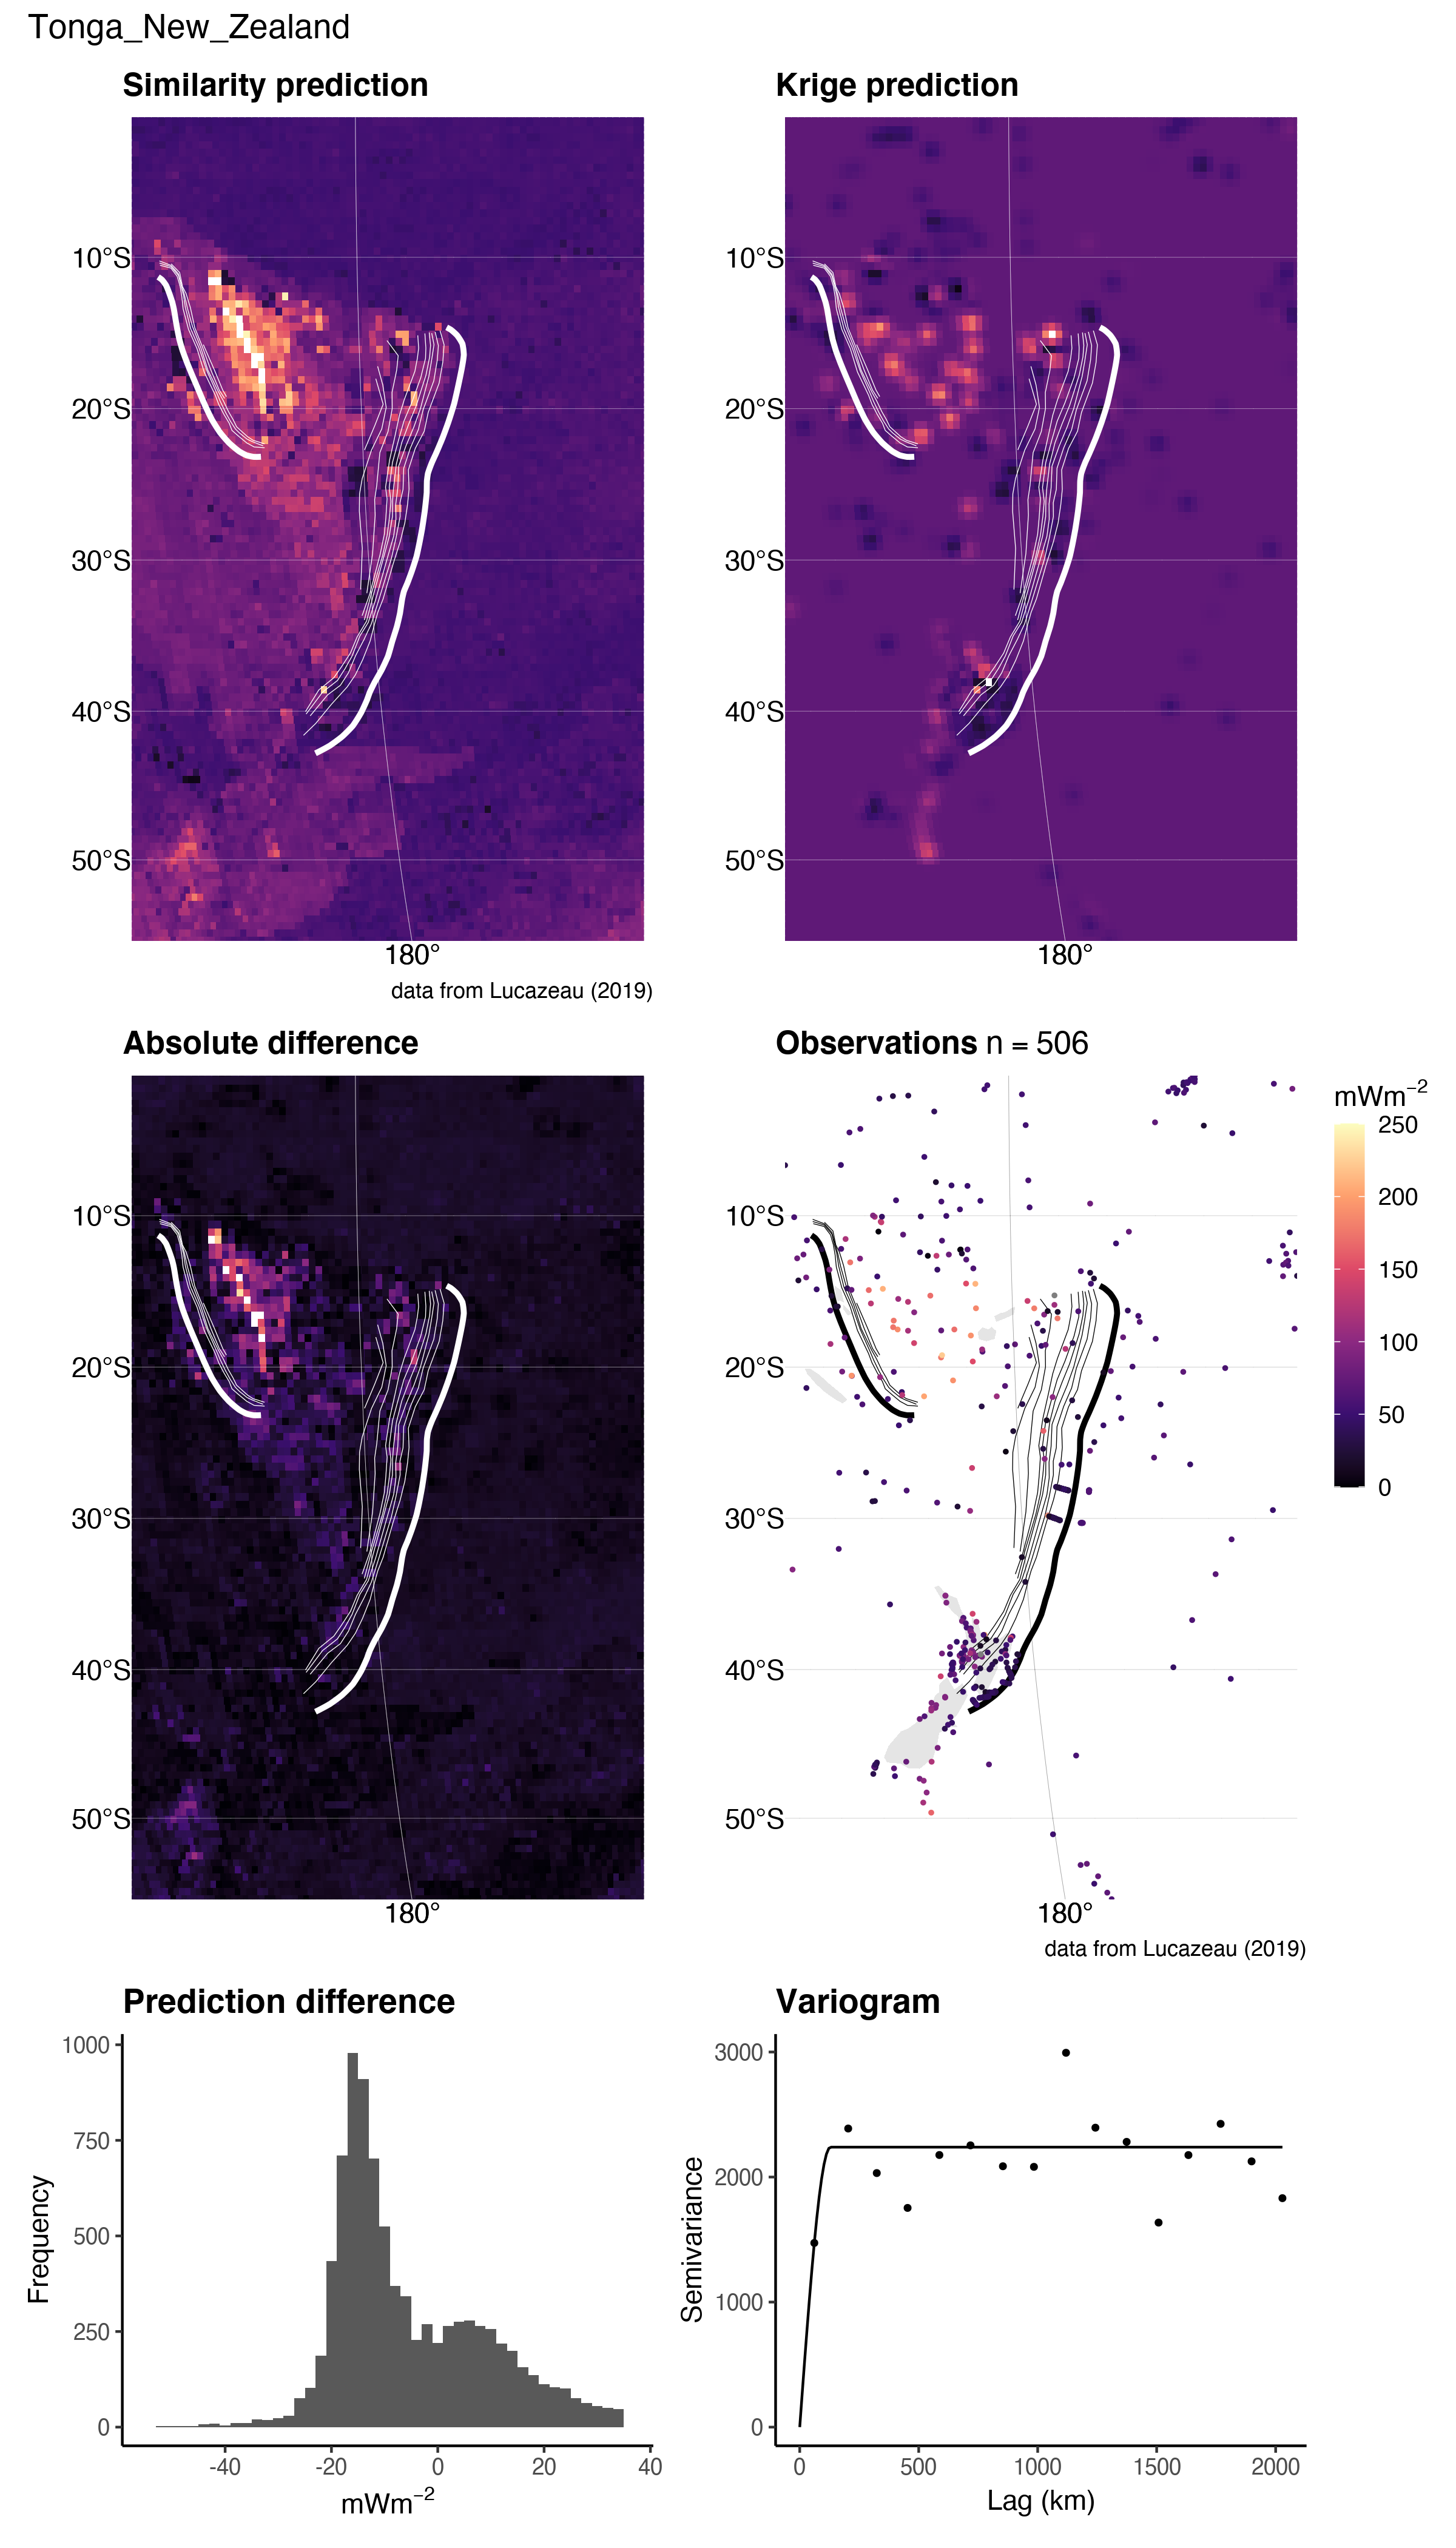
\includegraphics[width=0.95\linewidth,]{../figs/diff/comp/Tonga_New_Zealand} 

}

\caption{Similarity vs. Kriging predictions for Tonga New Zealand.}\label{fig:tonga.new.zealand.comp}
\end{figure}

\begin{figure}[h]

{\centering 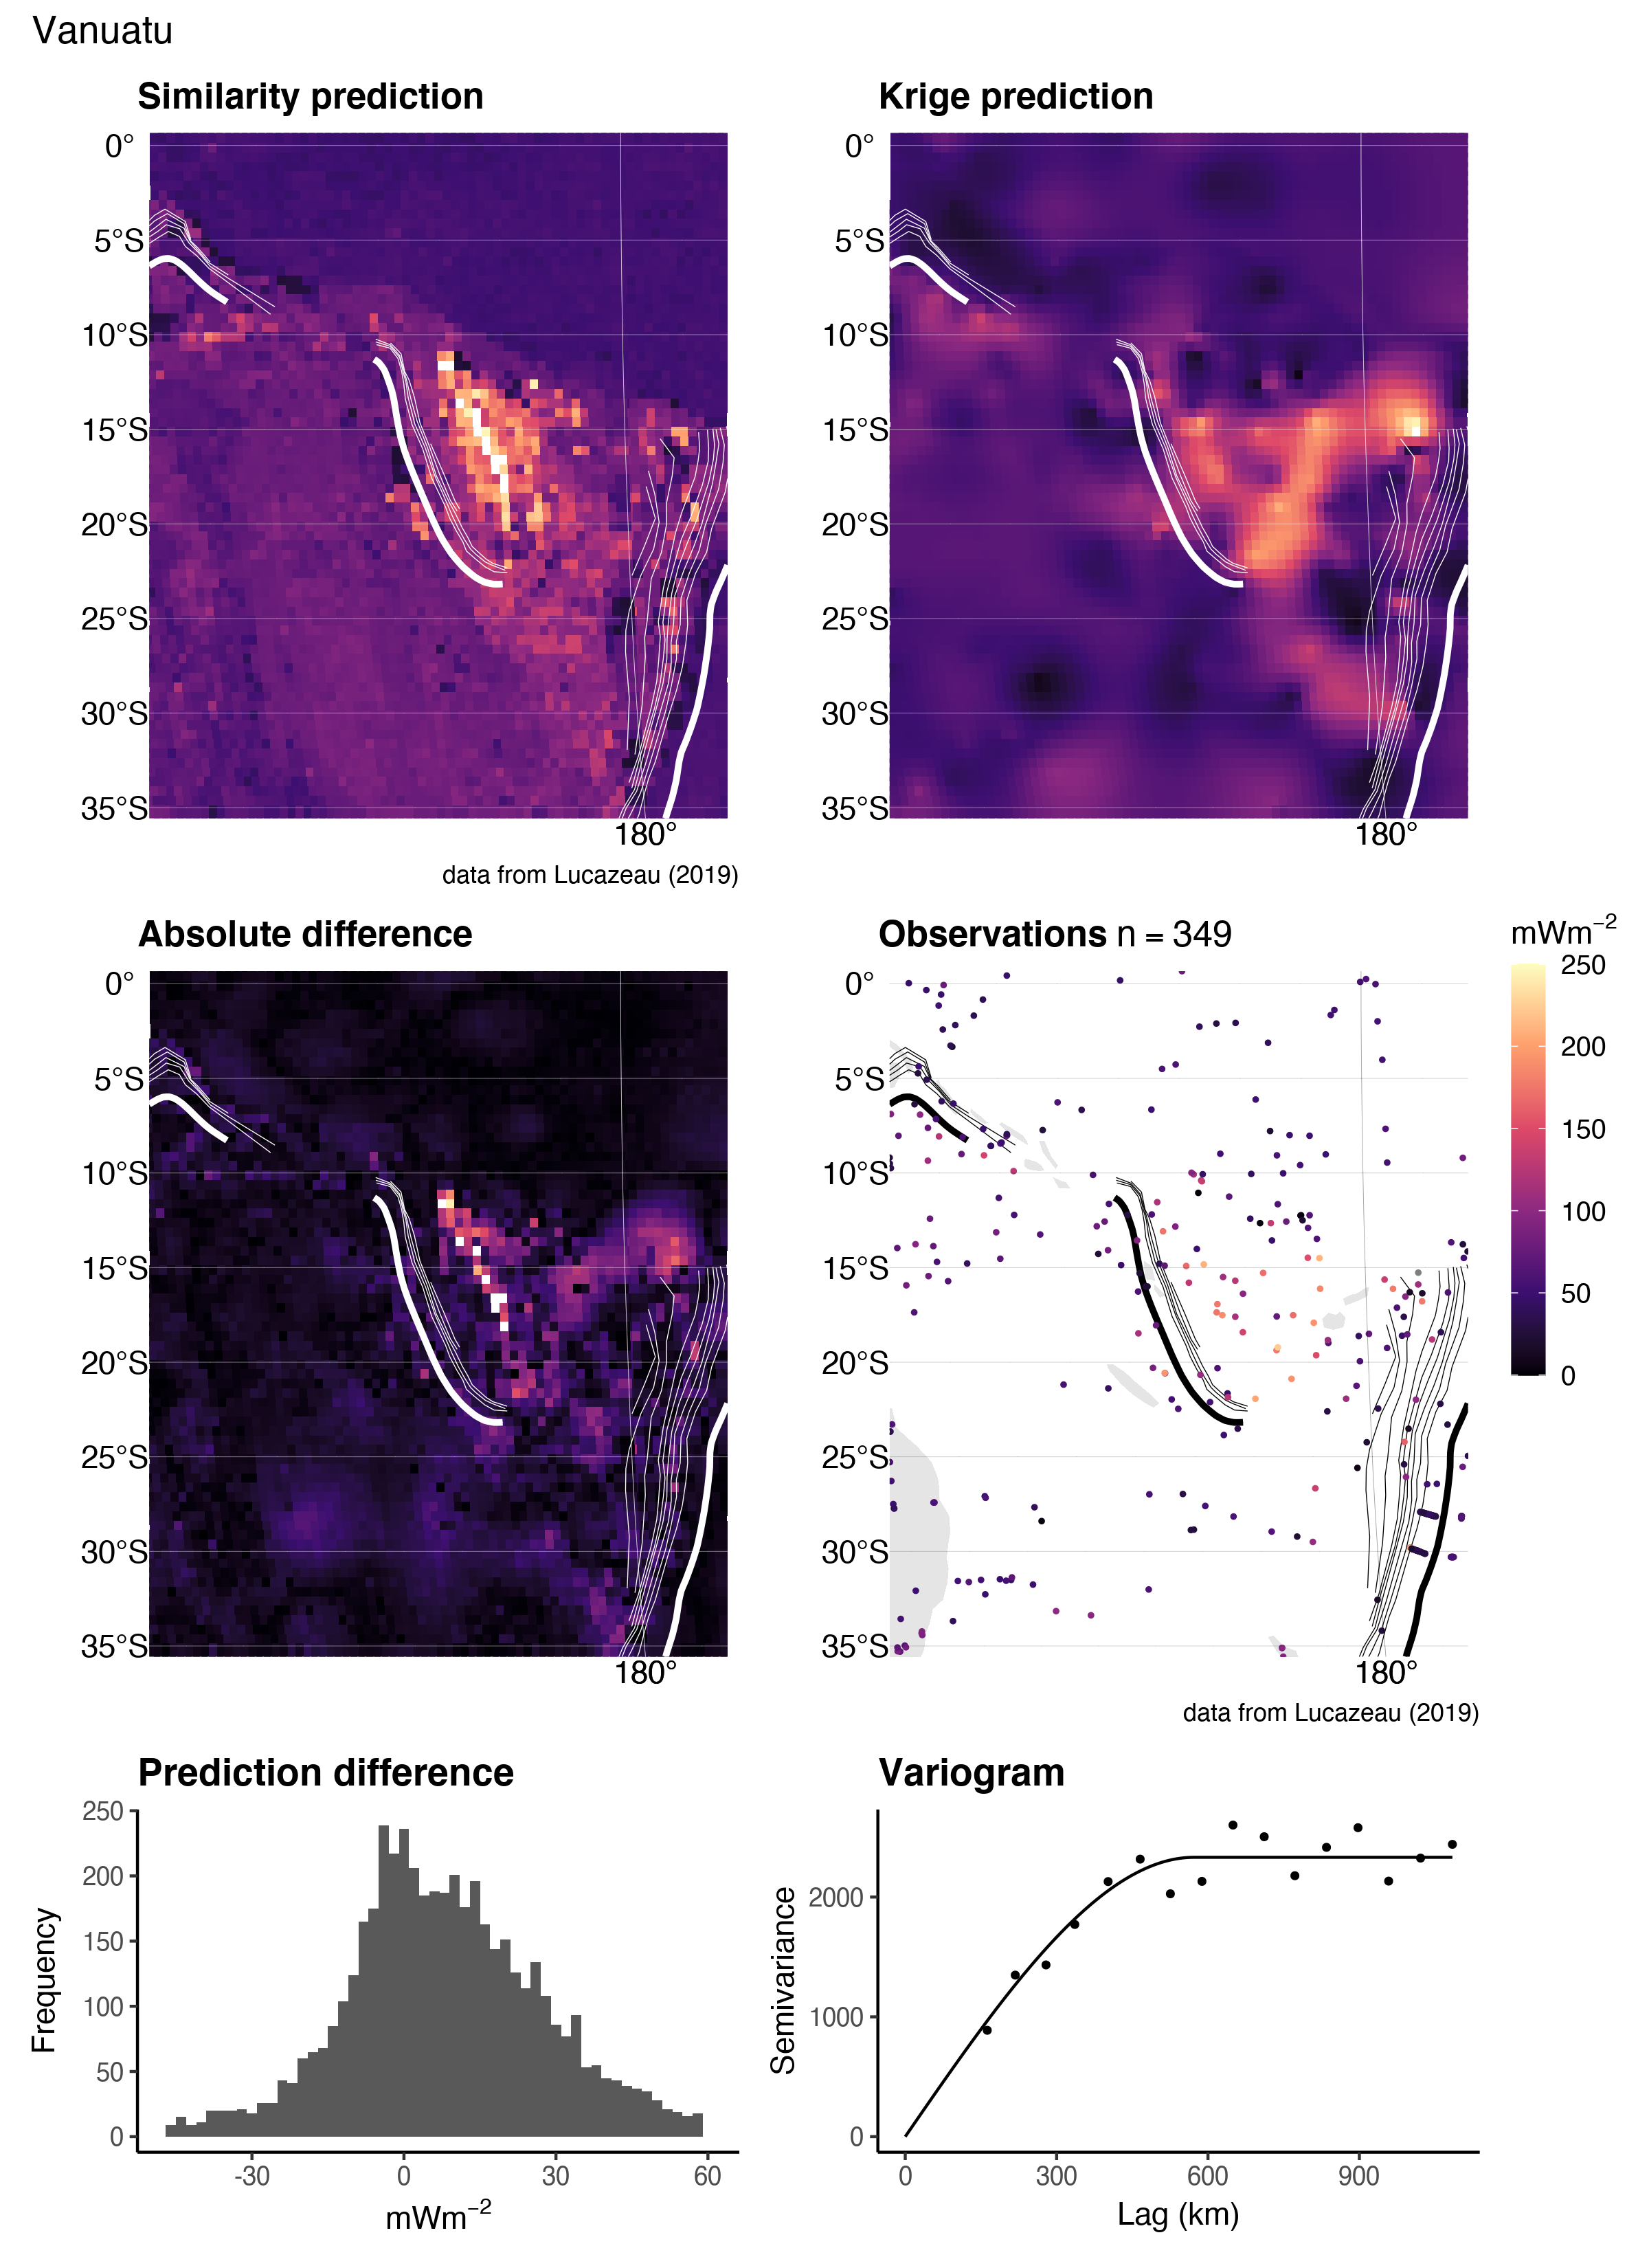
\includegraphics[width=0.95\linewidth,]{../figs/diff/comp/Vanuatu} 

}

\caption{Similarity vs. Kriging predictions for Vanuatu.}\label{fig:vanuatu.comp}
\end{figure}

\clearpage

\section*{References}
\addcontentsline{toc}{section}{References}

\hypertarget{refs}{}
\begin{CSLReferences}{1}{0}
\leavevmode\vadjust pre{\hypertarget{ref-bardossy1997}{}}%
Bárdossy, A. (1997). Introduction to geostatistics. \emph{Institute of
Hydraulic Engineering, University of Stuttgart}.

\leavevmode\vadjust pre{\hypertarget{ref-chapman1975}{}}%
Chapman, D. S., \& Pollack, H. N. (1975). Global heat flow: A new look.
\emph{Earth and Planetary Science Letters}, \emph{28}(1), 23--32.

\leavevmode\vadjust pre{\hypertarget{ref-chiles2009}{}}%
Chiles, J.-P., \& Delfiner, P. (2009). \emph{Geostatistics: Modeling
spatial uncertainty} (Vol. 497). John Wiley \& Sons.

\leavevmode\vadjust pre{\hypertarget{ref-cressie2015}{}}%
Cressie, N. (2015). \emph{Statistics for spatial data}. John Wiley \&
Sons.

\leavevmode\vadjust pre{\hypertarget{ref-currie2006}{}}%
Currie, C., \& Hyndman, R. D. (2006). The thermal structure of
subduction zone back arcs. \emph{Journal of Geophysical Research: Solid
Earth}, \emph{111}(B8).

\leavevmode\vadjust pre{\hypertarget{ref-currie2004}{}}%
Currie, C., Wang, K., Hyndman, R. D., \& He, J. (2004). The thermal
effects of steady-state slab-driven mantle flow above a subducting
plate: The cascadia subduction zone and backarc. \emph{Earth and
Planetary Science Letters}, \emph{223}(1-2), 35--48.

\leavevmode\vadjust pre{\hypertarget{ref-davies2013}{}}%
Davies, J. H. (2013). Global map of solid earth surface heat flow.
\emph{Geochemistry, Geophysics, Geosystems}, \emph{14}(10), 4608--4622.

\leavevmode\vadjust pre{\hypertarget{ref-fourier1827}{}}%
Fourier, J. (1827). M{é}moire sur les temp{é}ratures du globe terrestre
et des espaces plan{é}taires. \emph{M{é}moires de l'Acad{é}mie Royale
Des Sciences de l'Institut de France}, \emph{7}, 570--604.

\leavevmode\vadjust pre{\hypertarget{ref-furlong2013}{}}%
Furlong, K. P., \& Chapman, D. S. (2013). Heat flow, heat generation,
and the thermal state of the lithosphere. \emph{Annual Review of Earth
and Planetary Sciences}, \emph{41}, 385--410.

\leavevmode\vadjust pre{\hypertarget{ref-furukawa1993}{}}%
Furukawa, Y. (1993). Depth of the decoupling plate interface and thermal
structure under arcs. \emph{Journal of Geophysical Research: Solid
Earth}, \emph{98}(B11), 20005--20013.

\leavevmode\vadjust pre{\hypertarget{ref-gao2014}{}}%
Gao, X., \& Wang, K. (2014). Strength of stick-slip and creeping
subduction megathrusts from heat flow observations. \emph{Science},
\emph{345}(6200), 1038--1041.

\leavevmode\vadjust pre{\hypertarget{ref-goldberg1989}{}}%
Goldberg, D. E. (1989). Genetic algorithms in search.
\emph{Optimization, and MachineLearning}.

\leavevmode\vadjust pre{\hypertarget{ref-goodchild2004}{}}%
Goodchild, M. F. (2004). The validity and usefulness of laws in
geographic information science and geography. \emph{Annals of the
Association of American Geographers}, \emph{94}(2), 300--303.

\leavevmode\vadjust pre{\hypertarget{ref-goovaerts1997}{}}%
Goovaerts, P. (1997). \emph{Geostatistics for natural resources
evaluation}. Oxford University Press on Demand.

\leavevmode\vadjust pre{\hypertarget{ref-goutorbe2011}{}}%
Goutorbe, B., Poort, J., Lucazeau, F., \& Raillard, S. (2011). Global
heat flow trends resolved from multiple geological and geophysical
proxies. \emph{Geophysical Journal International}, \emph{187}(3),
1405--1419.

\leavevmode\vadjust pre{\hypertarget{ref-graler2016}{}}%
Gräler, B., Pebesma, E., \& Heuvelink, G. (2016). Spatio-temporal
interpolation using gstat. \emph{The R Journal}, \emph{8}, 204--218.
Retrieved from
\url{https://journal.r-project.org/archive/2016/RJ-2016-014/index.html}

\leavevmode\vadjust pre{\hypertarget{ref-hasterok2013}{}}%
Hasterok, D. (2013). A heat flow based cooling model for tectonic
plates. \emph{Earth and Planetary Science Letters}, \emph{361}, 34--43.

\leavevmode\vadjust pre{\hypertarget{ref-hasterok2008}{}}%
Hasterok, D., \& Chapman, D. (2008). Global heat flow: A new database
and a new approach. In \emph{AGU fall meeting abstracts} (Vol. 2008, pp.
T21C--1985).

\leavevmode\vadjust pre{\hypertarget{ref-hasterok2011}{}}%
Hasterok, D., Chapman, D., \& Davis, E. (2011). Oceanic heat flow:
Implications for global heat loss. \emph{Earth and Planetary Science
Letters}, \emph{311}(3-4), 386--395.

\leavevmode\vadjust pre{\hypertarget{ref-hyndman2005}{}}%
Hyndman, R. D., Currie, C. A., \& Mazzotti, S. P. (2005). Subduction
zone backarcs, mobile belts, and orogenic heat. \emph{GSA Today},
\emph{15}(2), 4--10.

\leavevmode\vadjust pre{\hypertarget{ref-jennings2021}{}}%
Jennings, S., \& Hasterok, D. (2021). HeatFlow.org. \emph{Heatflow.org}.
Retrieved from \url{http://heatflow.org/}

\leavevmode\vadjust pre{\hypertarget{ref-kerswell2020}{}}%
Kerswell, B. C., Kohn, M. J., \& Gerya, T. V. (2020). Backarc
lithospheric thickness and serpentine stability control slab-mantle
coupling depths in subduction zones. \emph{Earth and Space Science Open
Archive}, 34. \url{https://doi.org/10.1002/essoar.10503710.1}

\leavevmode\vadjust pre{\hypertarget{ref-krige1951}{}}%
Krige, D. G. (1951). A statistical approach to some basic mine valuation
problems on the witwatersrand. \emph{Journal of the Southern African
Institute of Mining and Metallurgy}, \emph{52}(6), 119--139.

\leavevmode\vadjust pre{\hypertarget{ref-lee1965}{}}%
Lee, W. H., \& Uyeda, S. (1965). Review of heat flow data.
\emph{Terrestrial Heat Flow}, \emph{8}, 87--190.

\leavevmode\vadjust pre{\hypertarget{ref-li2018}{}}%
Li, Z., Zhang, X., Clarke, K. C., Liu, G., \& Zhu, R. (2018). An
automatic variogram modeling method with high reliability fitness and
estimates. \emph{Computers \& Geosciences}, \emph{120}, 48--59.

\leavevmode\vadjust pre{\hypertarget{ref-lucazeau2019}{}}%
Lucazeau, F. (2019). Analysis and mapping of an updated terrestrial heat
flow data set. \emph{Geochemistry, Geophysics, Geosystems},
\emph{20}(8), 4001--4024.

\leavevmode\vadjust pre{\hypertarget{ref-matheron1963}{}}%
Matheron, G. (1963). Principles of geostatistics. \emph{Economic
Geology}, \emph{58}(8), 1246--1266.

\leavevmode\vadjust pre{\hypertarget{ref-matheron2019}{}}%
Matheron, G. (2019). \emph{Matheron's theory of regionalized variables}.
International Association for.

\leavevmode\vadjust pre{\hypertarget{ref-parsons1977}{}}%
Parsons, B., \& Sclater, J. G. (1977). An analysis of the variation of
ocean floor bathymetry and heat flow with age. \emph{Journal of
Geophysical Research}, \emph{82}(5), 803--827.

\leavevmode\vadjust pre{\hypertarget{ref-pebesma2004}{}}%
Pebesma, E. (2004). Multivariable geostatistics in {S}: The gstat
package. \emph{Computers \& Geosciences}, \emph{30}, 683--691.

\leavevmode\vadjust pre{\hypertarget{ref-pebesma2018}{}}%
Pebesma, E. (2018). {Simple Features for R: Standardized Support for
Spatial Vector Data}. \emph{{The R Journal}}, \emph{10}(1), 439--446.
\url{https://doi.org/10.32614/RJ-2018-009}

\leavevmode\vadjust pre{\hypertarget{ref-pollack1977}{}}%
Pollack, H. N., \& Chapman, D. S. (1977). On the regional variation of
heat flow, geotherms, and lithospheric thickness. \emph{Tectonophysics},
\emph{38}(3-4), 279--296.

\leavevmode\vadjust pre{\hypertarget{ref-pollack1993}{}}%
Pollack, H. N., Hurter, S. J., \& Johnson, J. R. (1993). Heat flow from
the earth's interior: Analysis of the global data set. \emph{Reviews of
Geophysics}, \emph{31}(3), 267--280.

\leavevmode\vadjust pre{\hypertarget{ref-proj2021}{}}%
PROJ contributors. (2021). \emph{{PROJ} coordinate transformation
software library}. Open Source Geospatial Foundation. Retrieved from
\url{https://proj.org/}

\leavevmode\vadjust pre{\hypertarget{ref-rudnick1998}{}}%
Rudnick, R. L., McDonough, W. F., \& O'Connell, R. J. (1998). Thermal
structure, thickness and composition of continental lithosphere.
\emph{Chemical Geology}, \emph{145}(3-4), 395--411.

\leavevmode\vadjust pre{\hypertarget{ref-sclater1970}{}}%
Sclater, J. G., \& Francheteau, J. (1970). The implications of
terrestrial heat flow observations on current tectonic and geochemical
models of the crust and upper mantle of the earth. \emph{Geophysical
Journal International}, \emph{20}(5), 509--542.

\leavevmode\vadjust pre{\hypertarget{ref-scrucca2013}{}}%
Scrucca, L. (2013). GA: A package for genetic algorithms in r.
\emph{Journal of Statistical Software}, \emph{53}(4), 1--37.

\leavevmode\vadjust pre{\hypertarget{ref-scrucca2016}{}}%
Scrucca, L. (2016). On some extensions to GA package: Hybrid
optimisation, parallelisation and islands evolution. \emph{arXiv
Preprint arXiv:1605.01931}.

\leavevmode\vadjust pre{\hypertarget{ref-shapiro2004}{}}%
Shapiro, N. M., \& Ritzwoller, M. H. (2004). Inferring surface heat flux
distributions guided by a global seismic model: Particular application
to antarctica. \emph{Earth and Planetary Science Letters},
\emph{223}(1-2), 213--224.

\leavevmode\vadjust pre{\hypertarget{ref-stein1992}{}}%
Stein, C. A., \& Stein, S. (1992). A model for the global variation in
oceanic depth and heat flow with lithospheric age. \emph{Nature},
\emph{359}(6391), 123--129.

\leavevmode\vadjust pre{\hypertarget{ref-stein1994}{}}%
Stein, C. A., \& Stein, S. (1994). Constraints on hydrothermal heat flux
through the oceanic lithosphere from global heat flow. \emph{Journal of
Geophysical Research: Solid Earth}, \emph{99}(B2), 3081--3095.

\leavevmode\vadjust pre{\hypertarget{ref-syracuse2006}{}}%
Syracuse, E. M., \& Abers, G. A. (2006). Global compilation of
variations in slab depth beneath arc volcanoes and implications.
\emph{Geochemistry, Geophysics, Geosystems}, \emph{7}(5).

\leavevmode\vadjust pre{\hypertarget{ref-wada2009}{}}%
Wada, I., \& Wang, K. (2009). Common depth of slab-mantle decoupling:
Reconciling diversity and uniformity of subduction zones.
\emph{Geochemistry, Geophysics, Geosystems}, \emph{10}(10).

\leavevmode\vadjust pre{\hypertarget{ref-wilkinson2016}{}}%
Wilkinson, M. D., Dumontier, M., Aalbersberg, Ij. J., Appleton, G.,
Axton, M., Baak, A., et al. (2016). The FAIR guiding principles for
scientific data management and stewardship. \emph{Scientific Data},
\emph{3}(1), 1--9.

\leavevmode\vadjust pre{\hypertarget{ref-zhu2018}{}}%
Zhu, A.-X., Lu, G., Liu, J., Qin, C.-Z., \& Zhou, C. (2018). Spatial
prediction based on third law of geography. \emph{Annals of GIS},
\emph{24}(4), 225--240.

\end{CSLReferences}

\bibliography{ref.bib}


\end{document}
